%\documentclass[11pt]{scrartcl}
\documentclass[11pt, numbers=noenddot]{scrreprt}

\usepackage[T1]{fontenc}
\usepackage[utf8]{inputenc}
%\usepackage[english]{babel}

\usepackage{graphicx}
\graphicspath{ 
	{../resources/imgs/},
	{../../data/plots/},
	{../../data/plots/dataset_evaluation/}
}

%\usepackage[backend=biber, style=ieee]{biblatex}
\usepackage[backend=bibtex, style=authoryear-comp, url=false]{biblatex}
%\newcommand{\citep}{\parencite}  % adds \citep alias for citing with parenthesis
\let\citef\cite  % makes \citef an alias for \cite
\let\cite\parencite  % makes \cite an alias for \parencite
\addbibresource{../resources/MA.bib}
\AtEveryBibitem{
%\ifentrytype{article}{
%    \clearfield{urlyear}
%}{}
%\ifentrytype{book}{
%    \clearfield{urlyear}
%}{}
%\ifentrytype{collection}{
%    \clearfield{urlyear}
%}{}
%\ifentrytype{incollection}{
%    \clearfield{urlyear}
%}{}
%\ifentrytype{inproceedings}{
%    \clearfield{urlyear}
%}{}
\ifentrytype{online}{
    \clearfield{urlyear}
}{}
}

\KOMAoptions{parskip=half}

\usepackage[margin=3cm]{geometry} % Adjust margins

\usepackage{soul}
\usepackage{todonotes}
\usepackage{amsmath}
\usepackage{amssymb}
\usepackage{hyperref}
\usepackage{cleveref}
\usepackage{caption}
\usepackage{subcaption}
\usepackage{booktabs}
\usepackage{pdfpages}
\usepackage{csquotes}
\usepackage{algorithm}
\usepackage{newfloat}
\usepackage{enumitem}
\usepackage{algpseudocode}
\usepackage{verbatim}
\usepackage{listings}
\usepackage{amssymb}
\usepackage{multirow}
\usepackage{multicol}
\usepackage[export]{adjustbox}
\usepackage[nonumberlist, nopostdot, acronym, toc]{glossaries}
\usepackage[german]{datetime2}
\usepackage{rotating}

%\setcounter{secnumdepth}{3}

%\usepackage{array}  % needed for '\newcolumntype' command
%\newcolumntype{L}[1]{>{\raggedright\arraybackslash}p{#1}}  % define "L" column type
%% Define a new counter for tracking the list number

% Counter for observation lists
\newcounter{listcounter}
\setcounter{listcounter}{0}

\DeclareFloatingEnvironment[
  listname = {List of Patterns} ,
  name = Pattern,
  placement = h,
  within = none
]{pattern}

\DeclareFloatingEnvironment[
  listname = {List of Hyperedges} ,
  name = Hyperedge,
  placement = h,
  within = none
]{hedge}

\Crefname{pattern}{Pattern}{Patterns}
\crefname{pattern}{pattern}{patterns}
\Crefname{hedge}{Hyperedge}{Hyperedges}
\crefname{hedge}{hyperedge}{hyperedges}


\lstset{
  language=Python,
  basicstyle=\ttfamily\small,  % Use small typewriter font
  columns=flexible,            % Use flexible spacing between characters
  captionpos=b,                % Place the caption below the listing
  frame=tb,                    % Add top and bottom frames to the listing
  keepspaces=true              % Preserve spaces in the code, useful for alignment
}

\DeclareFloatingEnvironment[
  listname = {List of Pseudocodes} ,
  name = Pseudocode,
  placement = h,
  within = none
]{pseudo}

\Crefname{pseudo}{Pseudocode}{Pseudocodes}
\crefname{pseudo}{pseudocode}{pseudocodes}


%\usepackage{lipsum}  % produces dummy text


% Load the glossary entries from an external file
\loadglsentries{glossary}
\makeglossaries

% Define a custom style for the first usage
\newacronymstyle{firstlong-emph}%
{%
  \GlsUseAcrEntryDispStyle{long-short}%
}%
{%
  \GlsUseAcrStyleDefs{long-short}%
  \renewcommand*{\genacrfullformat}[2]{%
    \emph{\glsentrylong{##1}} (\glsentryshort{##1})##2%
  }
  \renewcommand*{\Genacrfullformat}[2]{%
    \emph{\Glsentrylong{##1}} (\Glsentryshort{##1})##2%
  }
  \renewcommand*{\genplacrfullformat}[2]{%
    \emph{\glsentrylongpl{##1}} (\glsentryshortpl{##1})##2%
  }
  \renewcommand*{\Genplacrfullformat}[2]{%
    \emph{\Glsentrylongpl{##1}} (\glsentryshortpl{##1})##2%
  }
}

% Set the custom style
\setacronymstyle{firstlong-emph}


\begin{document}

% ========== poopy doopy



{\Large \textbf{Eigenständigkeitserklärung}} \\ \\
Hiermit versichere ich, dass ich die vorliegende Arbeit ohne Hilfe Dritter und ausschließlich unter Verwendung der aufgeführten Quellen und Hilfsmittel angefertigt habe. Alle Stellen, die aus den benutzten Quellen und Hilfsmitteln wörtlich oder inhaltlich übernommen sind, habe ich als solche kenntlich gemacht. Sofern KI-Tools verwendet wurden, habe ich Produktnamen, Hersteller, die jeweils verwendete Softwareversion und die Art der Nutzung (z.B. sprachliche Überprüfung und Verbesserung der Texte, systematische Recherche) benannt. Ich verantworte die Auswahl, die Übernahme und sämtliche Ergebnisse des von mir verwendeten KI-generierten Outputs vollumfänglich selbst. Die Satzung zur Sicherung guter wissenschaftlicher Praxis an der TU Berlin vom 8. März 2017 (https://www.static.tu.berlin/
fileadmin/www/10000060/FSC/Promotion\_\_Habilitation/Dokumente/Grundsaetze\_gu\\
te\_wissenschaftliche\_Praxis\_2017.pdf) habe ich zur Kenntnis genommen. Ich erkläre weiterhin, dass ich die Arbeit in gleicher oder ähnlicher Form noch keiner anderen Prüfungsbehörde vorgelegt habe.

Berlin, den \DTMtoday\\ \\
\includegraphics[width=200pt]{Unterschrift.png}\\
\noindent\rule{8cm}{0.4pt}\\
Unterschrift

\newpage
% ========== Title page

\titlehead
{
\begin{tabular}{ll}
\begin{minipage}{0.5\textwidth}
	\textbf{Technische Universität Berlin} \\
	Fakultät IV: Elektrotechnik und Informatik \\
	Institut für Telekommunikationssysteme \\
	Fachgebiet Verteilte offene Systeme	
\end{minipage}
&
\begin{minipage}{0.5\textwidth}
	\raggedleft
	
\includegraphics[width=0.3\textwidth]{logos/tub_logo_bw.jpg}			
\end{minipage}

\end{tabular}
}

\subject{Masters Thesis in Computer Science}
\title{Extending Semantic Hypergraphs by Neural Embedding-based Semantic Similarity for Pattern Matching}
\author{Max Reinhard \\ \small Matrikelnummer: 359417}

%\date{\today}
\date{\DTMtoday} % The date will be formatted in German style

\newcommand{\cmb}{\thanks{Centre Marc Bloch (An-Institut der Humboldt-Universität zu Berlin)}}
\newcommand{\fhfokus}{\thanks{Fraunhofer-Institut für offene Kommunikationssysteme}}

\publishers{Supervised by Prof. Dr. Manfred Hauswirth \\
	Additional guidance by Prof. Dr. Camille Roth\cmb, \\
	Dr. Telmo Menezes\footnotemark[1] \ and Dipl.-Math. Thilo Ernst\fhfokus
}
	
\maketitle

% ========== Abstract
\begin{abstract}
\textbf{Abstract}
This thesis introduces a novel enhancement to the Semantic Hypergraph (SH) framework's pattern matching capabilities through the integration of Neural Embedding-based Semantic Similarity (NESS). The SH framework utilises a symbolic and structured representation of text, combined with a pattern matching functionality that allows for open and explainable text analysis -- particularly aimed at Computational Social Science (CSS) researchers. Originally, the SH pattern matching follows strict, symbolic rules, with limited flexibility in matching the words that are integrated into the structured SH representation. Through incorporation of two NESS variants -- Fixed Word Embedding and Contextual Embedding-based measures -- the enhancement contributed in this work, allows for more semantically sophisticated patterns and therefore increases adaptivity of the pattern matching process. To provide partial control over the simultaneously introduced opaqueness, we enable users to configure crucial parameters of the NESS measurement. We conducted a comprehensive quantitative evaluation using a newly constructed labeled dataset to test the effectiveness of the NESS integration. The results demonstrate improved retrieval performance of the pattern matching, specifically showcasing the systems ability for contextual differentiation. Moreover, the implementation of the extended SH framework has been designed to be readily usable, facilitating its adoption for practical applications in CSS text analysis.
\end{abstract}


\begin{abstract}
\textbf{Zusammenfassung}
Diese Abschlussarbeit führt eine neuartige Verbesserung der Pattern-Matching-Fähigkeiten des Semantic Hypergraph (SH) Frameworks durch die Integration von Neural Embedding-basierter semantischer Ähnlichkeit (NESS) ein. Das SH-Framework nutzt eine symbolische und strukturierte Textrepräsentation, kombiniert mit einer Pattern-Matching-Funktionalität, die eine offene und erklärbare Textanalyse ermöglicht – insbesondere für Forscher im Bereich der Computational Social Science (CSS). Ursprünglich folgt das SH Pattern Matching strikten, symbolischen Regeln mit begrenzter Flexibilität bei der Übereinstimmung der Wörter, die in die strukturierte SH-Repräsenation integriert sind. Durch die Einbeziehung von zwei Varianten der NESS -- statische Wort-Embedding und kontextsensitive Emedding-basiert –- ermöglicht die in dieser Arbeit beigetragene Verbesserung komplexere semantische Patterns und erhöht somit die Anpassungsfähigkeit des Pattern-Matching-Prozesses. Um der gleichzeitig eingeführte Undurchsichtigkeit teilweise entgegenzuwirken, ermöglichen wir den Benutzern, entscheidende Parameter der NESS-Messung zu konfigurieren. Wir führten eine umfassende quantitative Auswertung mit einem neu erstellten, annotierten Datensatz durch, um die Effektivität der NESS-Integration zu testen. Die Ergebnisse zeigen eine verbesserte Retrieval-Leistung des Pattern Matching, insbesondere die Fähigkeit des Systems zur kontextuellen Differenzierung. Darüber hinaus wurde die Implementierung des erweiterten SH-Frameworks einfach zugäng-lich gestaltet, um eine praktische Anwendungen in der CSS-Textanalyse zu erleichtern.
\end{abstract}

% ========== TOC
\tableofcontents
\newpage

% ========== Body
% ==============================

% ========== 
\chapter{Introduction}

%\begin{itemize}
%	\item Context: The big problem
%	\item Problem statement: The small problem
%	\item Methodology / Strategy
%	\item Structure
%\end{itemize}
%
%\textbf{Notes:}
%\begin{itemize}
%	\item Huge amounts of text, which can provide insight about stuff
%	\item Automatic tools can provide assistance for humans to process all the text
%	\item This generally means filtering the original text corpus or otherwise reducing amount of information the information that has to be processed by humans
%	\item Filtering introduces a bias
%	\item Especially for scientific purposes it is relevant to mitigate bias or at least understand what bias has been introduced (to make it transparent)
%	\item Semantic Hypergraphs can be a valuable tool for that because...
%\end{itemize}
%
%
%Human life in times of widespread use of the internet and smartphones is most certainly more than ever interspersed with text-based communication...
%
%Great progress has been made in the made in NLP, IR and IE in the past decade. This advancement of the state-of-the-art can primarily be attributed \textit{Deep Learning} based methods, often also referred to as \textit{Neural Networks}. \cite{youngRecentTrendsDeep2018, minRecentAdvancesNatural2023, hirschbergAdvancesNaturalLanguage2015}
%
%open-opaque / strict-adaptive categorisation dimensions
%
%
%
%\section{Expose intro}
%
A significant part of the social world is nowadays being represented by digitally manifested text. Examples for this range from instant messaging, social media and any form of collective web activity to encyclopaedic websites, digitized libraries and government intelligence. The amount and richness of available social text makes it a valuable data source for social science research, while simultaneously creating an interest in automatic systems to analyze these texts on a large scale \cite{evansMachineTranslationMining2016}. Such research can be understood as part of the domain of \gls{css} \cite{lazerComputationalSocialScience2009}.

Systems based on techniques from the field of \gls{nlp}, as well well as the interlinked fields of \gls{ir} and \gls{ie}, have demonstrated great success in a variety of task related to text analysis. This success is largely attributed to the advancements of applying of \gls{ml}  and especially \gls{dl} methods to text \cite{hirschbergAdvancesNaturalLanguage2015, qiuPretrainedModelsNatural2020}. While being very effective at predicting or decision making, \gls{ml}- and specifically \gls{dl}-based systems generally do not deliver an explanation for their judgement and can mostly be viewed as "black box models" that are not transparent in their prediction or decision making process \cite{rudinStopExplainingBlack2019}. Conversely this transparency and explainability is of high interest in \gls{css} applications such as predicting political opinion based on social media activity \cite{wilkersonLargeScaleComputerizedText2017}.

The characteristic of \textit{openness} -- i.e. transparency and explainability -- in text analysis systems typically conflicts with \textit{adaptivity}, which refers to the capacity to learn and alter behaviour. This trade-off arises because adaptive systems frequently depend on \gls{ml} or \gls{dl} models, which are most often inherently \textit{opaque}. In contrast, systems that are \textit{open} are usually rule-based, making them principally \textit{strict} in their operation.

The \gls{sh} \cite{menezesSemanticHypergraphs2021} is a framework for representing and analyzing \gls{nl}. NL sentences can be modelled as an ordered, recursive hypergraph of hyperedges, which can be represented in a formal language. Based on this, the framework allows to specify semantic patterns in a pattern language, which can be matched against an existing \gls{sh}.
It aims to provide an \textit{open} and \textit{adaptive} system to analyse text corpora, especially in the domain of \gls{css}. The framework is open in the sense that its representation formalism is inspectable and intelligible by humans and that the pattern matching follows explicit rules. It is adaptive in the sense that its parsing is built from ML-based subsystems and therefore allows for an error-tolerant tranlataion from \gls{nl} to \gls{sh} in regards to grammatical and syntactical correctness.

While the \gls{sh} representation and its construction can be considered to fulfil the open-adaptive properties, the framework's pattern matching is purely symbolic and follows a set of fixed rules. It can therefore be considered to be \textit{open-strict}. The \gls{sh} pattern defined by a user may -- among other things -- specify the structure of the hyperedges that should match it and allows  to describe different levels of generalisations for the structural matching. In the \gls{sh} framework's original form, there is no possibility to define semantically sophisticated generalisations for the matching of hyperedge content, i.e. actual words that are contained within the text that is represented by an hyperedge.

By extending the the \gls{sh} matching process with the capability to utilize some form of semantic similarity in regard to edge content, we allow the \gls{sh} framework's users to define patterns, which describe such semantically sophisticated generalisations of edge content.
There exists a great variety of approaches for determining the semantic similarity of text \cite{harispeSemanticSimilarityNatural2015, chandrasekaranEvolutionSemanticSimilarity2021}. In this work, we identify \gls{ness} measures to be best suited for an integration into the \gls{sh} pattern matching. Since \gls{ness} measures are generally based on machine learning methods and sometimes based on deep neural network, they principally do not provide the openness that is inherent to the purely symbolic pattern matching process.

 In the sense of the open-opaque / strict-adaptive classification, this integration means a shift from openness to opaqueness and from strictness to adaptivity. To counteract the opaqueness introduced by an \gls{ness} integration into the \gls{sh} pattern matching, we allow user control over the generalisation level via the configuration of a similarity threshold, the ability to choose between fixed word and contextual neural embedding-based semantic similarity, and the option to toggle sub-edge specificity of the contextual embeddings. Therefore mantaining some openness while still benefiting from increased adaptivity.

In the context of this thesis, \gls{ness-shpm} is conceptualised and implemented by integrating it into the existing software package \textit{graphbrain}\footnote{graphbrain: \url{https://graphbrain.net/}}. Additionally it is subjected to a comprehensive quantitative evaluation regarding its retrieval performance on a newly constructed dataset comprised of labeled news headers.

The rest of this thesis is structured as follows: \Cref{cha:background} introduces the necessary background in regards to the Semantic Hypergraph framework and discusses the state-of-the-art of semantic similarity measures. \Cref{cha:problem-statement} outlines the problem introduced earlier in more detail and formulates the subsequent research questions. \Cref{cha:solution-approach} devises the concept of \gls{ness-shpm} as approach to solving the stated problem. \Cref{cha:implementation} describes the specific software implementation of the proposed solution. \Cref{cha:evaluation} provides a thorough quantitive evaluation of the implemented system and discusses the results. 
\Cref{cha:conclusion} concludes this thesis by presenting the contributions made herein and suggesting possible avenues for further work.

% ========== 
\chapter{Background}
\glsreset{sh}
\glsreset{ness}
\glsreset{ss}
\glsreset{sr}

\label{cha:background}
In this chapter the necessary background for this work is presented. This includes on the one hand the \gls{sh} framework and its pattern matching capabilities in particular. On the other hand the concept of \gls{sr} and specifically \gls{ss} is discussed with a focus on its realisation in the form of \gls{ness}.

\section{Semantic Hypergraph Framework}
\label{sec:semantic-hypergraph-framework}

The Semantic Hypergraph framework, introduced in \citef{menezesSemanticHypergraphs2021}, offers a novel approach for the representation and analysis of \gls{nl} text. At its core, the \gls{sh} framework transforms text into a structured, symbolic format, thereby facilitating the analysis of text collections. A pattern language intrinsic to the \gls{sh} framework enables the definition of patterns that encapsulate generalisations of text in the \gls{sh} format.

Designed primarily for \gls{css} researchers, the \gls{sh} framework emphasises a high degree of openness, encompassing transparency and explainability. Additionally, the \gls{sh} framework exhibits a level of adaptiveness, attributing to its reliance on \gls{ml} components for the translation of \gls{nl} text into the \gls{sh} format. This adaptiveness reflects the framework's capability to evolve and accommodate the variable form of natural language.

One of the objectives of the \gls{sh} framework is to bridge the existing gap in open-adaptive \gls{nlp} systems. By providing a mechanism for structured symbolic representation and pattern-based analysis of text, the \gls{sh} framework proposes a solution that combines the benefits of machine learning adaptiveness with the requisites of open and explainable research in \gls{css} and beyond.

For a more comprehensive description of the Semantic Hypergraph framework, the original publication \cite{menezesSemanticHypergraphs2021} should be consulted.


\subsection{Structure and Syntax}
In the \gls{sh} framework, natural language is represented as a recursive, ordered \textit{hypergraph} (in the following also referred to as \textit{graph}). Such a hypergraph consists of \textit{hyperedges} (in the following also referred to as \textit{edges}). These hyperedges themselves can consist of a generally unrestricted number of hyperedges. To denote the hierarchy between hyperedges the terms \textit{parent edge} and \textit{child edge} or \textit{sub edge} are introduced. If an edge \(e_A\) contains edges \(e_B\) and \(e_C\), \(e_A\) is considered to be the parent edge of child or sub edges \(e_B\) and \(e_C\). Since hyperedges are ordered, the edge \(e_A = (e_B \ e_C)\) is different to an edge \((e_C \  e_B) \neq e_A\). If a hyperedge is not a composition of multiple hyperedges, it is called an \textit{atom}.


\subsubsection{Hyperedge Examples}
Some example phrases and their corresponding hyperedges are given to help illustrate the general concept of the hypergraph representation and the hyperedge notation:

\begin{itemize}
	\item "banana": \textsf{banana/C}, "eat": \textsf{eat/C}, "sweet": \textsf{sweet/C}
	\item "Mango is tasty.": \textsf{(is/P.sc mango/C tasty/C)}
	\item "Sophie throws the ball.": \textsf{(throws/P.so sophie/C (the/M ball/C))}
\end{itemize}


\subsubsection{Hyperedge Components and Notation}
\label{sec:hyperedge-notation}
An atomic hyperedge is noted as follows:

\begin{center}
	\texttt{<CONTENT>}\textsf{/}\texttt{<TYPE>} or \\
	\texttt{<CONTENT>}\textsf{/}\texttt{<TYPE>}\textsf{.}\texttt{<ARGUMENT ROLES>}
\end{center}

The different edge components \textit{content}, \textit{type} and potentially \textit{argument roles} are here represented by placeholders in brackets (\texttt{<>}). In an atom, the content is always noted in lowercase. Non-atomic hyperedges are noted as a composition of their sub edges, as illustrated above. They also always have content and type, which are not part of the notation, but can be inferred. Each of the hyperedge components is explained in the following.

\subsubsection{Hyperedge Types}
Every hyperedge in a semantic hypergraph has a specific type. All types that an edge can assume are listed in \cref{tab:hyperedge-types}, which is adapted from \citef[p. 7]{menezesSemanticHypergraphs2021}.

\begin{table}[h]
\centering
\begin{tabular}{clp{5cm}l}
\toprule
\textbf{Code} & \textbf{Type} & \textbf{Purpose} & \textbf{Example} \\
\midrule
\textsf{C} & Concept & Define atomic concepts & \textbf{\textsf{apple/C}} \\
\textsf{P} & Predicate & Build relations & \textsf{(\textbf{is/P} berlin/C nice/C)} \\
\textsf{M} & Modifier & Modify a concept, predicate, modifier, trigger & \textsf{(\textbf{red/M} shoes/C)} \\
\textsf{B} & Builder & Build concepts from concepts & \textsf{(\textbf{of/B} capital/C germany/C)} \\
\textsf{T} & Trigger & Build specifications & \textsf{(\textbf{in/T} 1994/C)} \\
\textsf{J} & Conjunction & Define sequences of concepts or relations & \textsf{(\textbf{and/J} meat/C potatoes/C)} \\
\textsf{R} & Relation & Express facts, statements, questions, orders, ... & \textsf{\textbf{(is/P berlin/C nice/C)}} \\
\textsf{S} & Specifier & Relation specification (e.g., condition, time, ...) & \textsf{\textbf{(in/T 1976/C)}} \\
\bottomrule
\end{tabular}
\caption{Hyperedge types with their purpose and examples. For the examples the sub edge(s) that correspond(s) to the respective type is noted in bold face.}
\label{tab:hyperedge-types}
\end{table}

%\begin{table}[ht]
%\centering
%\begin{tabular}{clccc}
%\toprule
%\textbf{Code} & \textbf{Type} & \textbf{Connector} & \multicolumn{2}{c}{\textbf{Atomicity}} \\
%              &               &               & \textbf{Atom} & \textbf{Non-atom} \\
%\midrule
%\textsf{C}    & Concept       &               & \checkmark & \checkmark \\
%\textsf{P}    & Predicate     & \checkmark    & \checkmark & \checkmark \\
%\textsf{M}    & Modifier      & \checkmark    & \checkmark & \checkmark \\
%\textsf{B}    & Builder       & \checkmark    & \checkmark &            \\
%\textsf{T}    & Trigger       & \checkmark    & \checkmark &            \\
%\textsf{J}    & Conjunction   & \checkmark    & \checkmark &            \\
%\textsf{R}    & Relation      &               &            & \checkmark \\
%\textsf{S}    & Specifier     &               &            & \checkmark \\
%\bottomrule
%\end{tabular}
%\caption{Hyperedge types with their connector status and atomicity.}
%\label{table:hyperedge_types}
%\end{table}

\paragraph{Type Inference Rules}
The type of a parent hyperedge is inferred based on the types and the order of its child hyperedges following specific inference rules. These rules can be inspected in \citef[p. 8]{menezesSemanticHypergraphs2021}, but are omitted here, because they are deemed mostly irrelevant for this work.


\subsubsection{Hyperedge Content}
The textual representation of an edge is referred to as \textit{edge content} or \textit{edge text}. For atoms this is generally a word, except for semantically relevant punctuation characters and special symbols (see below). Generally speaking, a hyperedges content is the reconstruction of the word, phrase or sentence that it represents, which can be produced by following the hyperedge structure.

\paragraph{Special Content Symbols}
\label{sec:special-type-symbols}
The content of edges of the builder and conjunction type can also take on the form of special symbols \textsf{+/B} and \textsf{:/J}. This is utilised to represent phrases where there is no (meaningful) word or character attributable to the edges content. Examples of this are (taken from \citef[p. 7]{menezesSemanticHypergraphs2021}):

\begin{itemize}
	\item "guitar player": \textsf{(+/B guitar/C player/C)}
	\item "Freud, the famous psychiatrist": \textsf{(:/J freud/C (the/M (famous/M psychiatrist/C)))}
\end{itemize}


\subsubsection{Argument Roles}
To make the meaning of the relation of sub edges in a parent edge more explicit, builder and predicate edges can have argument roles. In parent edges that start with an edge of one of these two types, the roles of the other edges can be specified by adding argument roles to the builder or predicate edges. These are denoted as shown in \cref{sec:hyperedge-notation}.
%We only list the possible argument roles here to avoid confusing the reader, since they are used in some of the edges and patterns in the following, but they are not in the focus of this work. 
A table of all possible argument roles and an explanation of their functionality can be inspected in \citef[p. 8]{menezesSemanticHypergraphs2021}, but they are not in the focus this work.


\subsection{Translation Process}
\label{sec:sh-translation-process}
For natural language text to be represented in the Semantic Hypergraph framework, it needs to be translated (or parsed). This aspect of the framework is mostly irrelevant for this work and is therefore only described briefly here. The translation is realised by machine learning based software components. This is a high-level description of the process: 

\begin{enumerate}
	\item Segment text into sentences and tokenise sentences
	\item Annotate tokens with POS-tags, dependency labels and NER categories
	\item Use a trained classification model to predict an atom edge type for a token using its annotation labels as input features
	\item Recursively construct more complex hyperedges from the sequence of atomic edges by essentially applying the type inference rules
\end{enumerate}

The edges that correspond to the sentences into which the original input text has been segmented are referred to as \textit{root edges} of a graph in the following. 


\subsection{Pattern Matching}
\label{sec:sh-pattern-matching}
Text represented in the \gls{sh} framework can be analysed via \gls{shpm}. Information can be extracted from texts represented as hypergraph by constructing patterns in the frameworks pattern language and matching these patterns against the graph. The extracted information can take on the form of e.g. specific kinds of expressions and parts of these expression that fulfil a certain role.


\subsubsection{Pattern Language}
\label{sec:sh-pattern-language}
The \gls{shpl} essentially allows for generalisations of hyperedge structure and content. All valid hyperedges are generally also valid patterns in the \gls{shpl}. \Cref{tab:pattern-language-elements} list all of the pattern languages elements (also referred to as operators), which are relevant to this work. Their functionality and therefore the form of generalisation that they enable is also described.

\begin{table}[h]
\centering
\begin{tabular}{lcp{9cm}}
\toprule
\textbf{Element} & \textbf{Notation} & \textbf{Function} \\
\midrule
Variable & \textsf{VAR} & Matches any edge (restrictable by type and argument roles). Returns the edge that it captures. \\
Wildcard & \textsf{*} & Matches any edge (restrictable by type and argument roles). \\
Options list & \textsf{[...]} & Matches one of the given options. Applicable to edge type and content. \\
Innermost atom & \textsf{>} & Matches against the innermost atom of the edge that it captures. Removes an arbitrary level of nested modifiers. \\
Lemma function & \textsf{lemma} & Matches if the lemma of the captured edge content equals the given word. Combinable with an options list. Applicable only to atoms. \\
Argument role set & \textsf{\{\(\alpha\beta\gamma, \epsilon\)\}} & Allows for argument roles in arbitrary order. Comma-separated argument roles are optional \\
\bottomrule
\end{tabular}
\caption{Pattern language elements with their notation and function}
\label{tab:pattern-language-elements}
\end{table}

\subsubsection{Matching Process}
\label{sec:pattern-matching-process}
At its core, the matching process involves comparing a predefined pattern against either an entire hypergraph, a set of edges, or a single edge. Independent of the matching target, this comparison is conducted one edge at a time, determining whether this edge aligns with the pattern. If pattern and edge do not match, the result of this process is only the binary information of \textit{No Match}. If pattern and edge do match, the result of the matching process depends on whether the pattern contains variables. I this case, the result is not only the binary information of \textit{Match}, but also the assignment of the variables contained in the pattern. It is possible for a single edge to yield multiple variable assignments, however this aspect will not be discussed further as it holds limited relevance for this work. 

The matching process works recursively, processing both the structure and content of the edge in relation to the pattern. If a generalising part of the pattern (sub pattern) structurally matches a sub edge of the candidate edge, this sub edge is considered to be \textit{captured} by this sub pattern. This is relevant for returning variable assignments and further processing, as is needed for the innermost atom operator or any content generalisation functionality.

Assuming the matching process is examining a specific sub pattern and sub edge, the content defined in the sub pattern is referred to as the \textit{(pattern) reference content}. It is worth noting that a pattern may exclusively consist of structural elements, without specifying content. The content of the sub edge under comparison is termed as the \textit{(edge) candidate content}. Apart of structural matching, the process also involves a comparison between the reference content and the candidate content, employing either a direct string-based comparison or comparing the candidate words lemma against the reference word(s).

Edge argument roles are ignored when matching, if they are not specified in a pattern. The matching of argument roles is not elaborated further, as it is of little relevance here.


\paragraph{Example Matchings} To illustrate the expressiveness and of the \gls{shpl} and the
functionalities of the different language elements, some example matchings of patterns against edges are shown in \cref{tab:shpl-example-matchings}. The corresponding edges and patterns are listed below.

\paragraph{Example Edges}
\begin{enumerate}[label={$e_{\arabic*}$ = }]
	\item \textsf{( plays/P.so ann/C ( acoustic/M guitar/C ) )}
	\item \textsf{( plays/P.so ann/C ( acoustic/M piano/C ) )}
	\item \textsf{( plays/P.so ann/C ( aggressive/M rugby/C ) )}
	\item \textsf{( plays/P.sx ann/C ( if/T ( has/P.so she/C time/C ) ) )}
	\item \textsf{( play/P.so ( and/J ann/C bob/C ) ( a/M song/C ) )}
	\item \textsf{( ( again/M perform/P.so ) they/C ( the/M ( same/M song/C ) ) )}
\end{enumerate}


\paragraph{Example Patterns}
%\begin{multicols}{2}
\begin{enumerate}[label={$p_{\arabic*}$ = }]
	\item \textsf{( plays/P PERS/C THING/C )}
	\item \textsf{( plays/P ann/C * )} 
	\item \textsf{( plays/P ann/C VAR/[CS] )}
	\item \textsf{( plays/P ann/C >[guitar, piano]/C )}
	\item \textsf{( plays/P ann/C >THING/C )}
	\item \textsf{( plays/P ann/C ( >IN\gls{st}/C [guitar, piano] ) )}
	\item \textsf{( ( lemma play/P ) ACTOR/C THING/C )}
	\item \textsf{( ( lemma >[play, perform]/P ) ACTOR/C THING/C )}
\end{enumerate}
%\end{multicols}

%\paragraph{Example Patterns}
%\begin{enumerate}
%	\item \textsf{(plays/P PERS/C IN\gls{st}/C)} utilises variables
%	\item \textsf{(plays/P ann/C *)} utilises wildcard
%	\item \textsf{(plays/P ann/C VAR/[CS])}  utilises variable and type options list
%	\item \textsf{(plays/P ann/C >[guitar, piano]/[CS])} utilises innermost atom, type options list and content options list
%	\item \textsf{(plays/P ann/C >IN\gls{st}/[CS])} utilises innermost variables, innermost atom and type options list
%	\item \textsf{(plays/P ann/C (>IN\gls{st}/[CS] [guitar, piano]))} utilises variable, innermost atom, type options list and content options list
%\end{enumerate}

%\vspace{\baselineskip}
\begin{table}[ht]
\centering
\begin{tabular}{cccl}
\toprule
\textbf{Pattern} & \textbf{Edge} & \textbf{Match?} & \textbf{Variables} \\
\midrule
\(p_1\) & \(e_1\) & \textit{Match} & \textsf{PERS=ann/C, THING=(acoustic/M guitar/C)} \\
\(p_1\) & \(e_4\) & \textit{No Match} & \\
\(p_2\) & \(e_1\), \(e_2\), \(e_3\), \(e_4\) & \textit{Match} & \\
\(p_2\) & \(e_5\), \(e_6\) & \textit{No Match} & \\
\(p_3\) & \(e_1\) & \textit{Match} & \textsf{VAR=(acoustic/M guitar/C)} \\
\(p_3\) & \(e_4\) & \textit{Match} & \textsf{VAR=if/T (has/P.so she/C time/C)} \\
\(p_4\) & \(e_1\), \(e_2\) & \textit{Match} & \\
\(p_4\) & \(e_3\), \(e_4\)  & \textit{No Match} & \\
\(p_5\) & \(e_1\)  & \textit{Match} & \textsf{THING=guitar/C} \\
\(p_5\) & \(e_3\)  & \textit{Match} & \textsf{THING=rugby/C} \\
\(p_5\) & \(e_4\)  & \textit{No Match} & \\
\(p_6\) & \(e_2\)  & \textit{Match} & \textsf{IN\gls{st}=piano/C} \\
\(p_6\) & \(e_3, e_4\)  & \textit{No Match} & \\
\(p_7\) & \(e_1\)  & \textit{Match} & \textsf{ACTOR=ann/C, THING=(acoustic/C guitar/C)}\\
\(p_7\) & \(e_5\)  & \textit{Match} & \textsf{ACTOR=(and/J ann/C bob/C), THING=(the/M song/C)}\\
\(p_7\) & \(e_6\)  & \textit{No Match} & \\
\(p_8\) & \(e_6\)  & \textit{Match} & \textsf{ACTOR=they/C, THING=(the/M (same/M song/C)}\\
\bottomrule
\end{tabular}
\caption{Example matchings of patterns against edges}
\label{tab:shpl-example-matchings}
\vspace{2\baselineskip}
\end{table}



\section{Semantic Similarity Measures}
\label{sec:semantic-similarity}
\glsreset{sr}
\glsreset{ss}
\glsreset{kbss}
\glsreset{cbss}
\glsreset{ness}


Determining the \gls{sr} \gls{ss} of two text items is a central task in the interlinked fields of natural language processing, information retrieval and information extraction. A text item can take on the form of a word, phrase, sentence paragraph or entire document. While \gls{sr} and \gls{ss} are often used synonymously, semantic relatedness can also be understood to entail a more nuanced description of the semantic relations of text items \cite{chandrasekaranEvolutionSemanticSimilarity2021, harispeSemanticSimilarityNatural2015}.  In this work, the term \textit{Semantic Similarity} is therefore used to refer to the task of measuring the closeness, distance or similarity in regard to the meanings conveyed by two text items. This has to be differentiated from lexical (i.e. string-based) similarity measures, which in principle do not rely on the meaning of text items \cite{p.SurveySemanticSimilarity2019}. 

There exists a great variety of approaches to measuring semantic similarity and their categorisation also takes on different forms in the literature.
%A structure that is in line with most of the reviewed literature employs the following categories: \textit{Knowledge-based Semantic Similarity} (\gls{kbss}), \textit{Distributional} or \textit{Corpus-based Semantic Similarity} (\gls{cbss}), \textit{Deep Learning-} or \textit{Neural Network-based Semantic Similarity} (NN\gls{ss}) and hybrid approaches which combine techniques from multiple categories 
A structure that is in line with most of the reviewed literature employs the following categories: \gls{kbss} (see \cref{sec:knowledge-based-semantic-similarity}), \gls{cbss} (see \cref{sec:corpus-based-semantic-similarity}) and hybrid approaches which combine techniques from both categories
\cite{chandrasekaranEvolutionSemanticSimilarity2021, harispeSemanticSimilarityNatural2015, hanSurveyTechniquesApplications2021, zadSurveyDeepLearning2021}.

The focus of this work in assessing the state-of-the-art of semantic similarity measures lies on \gls{cbss} -- specifically a subform of corpus-based measures that is denoted here as \gls{ness} (see \cref{sec:neural-embedding-based-semantic-similarity-measurement}). These measures share some commonality with \gls{dlss}, which is sometimes differentiated as an independent category in the literature (see \cref{sec:deep-learning-based-semantic-similarity}).

\subsection{Knowledge-based Semantic Similarity}
\label{sec:knowledge-based-semantic-similarity}
Knowledges-based semantic similarity measures rely on some form of underlying structured knowledge source to compute the similarity between two text items. These knowledge sources (referred to as knowledge systems in the following) may be ontologies, knowledge bases, knowledge graphs, semantic graphs, (lexical) databases and similar systems \cite{chandrasekaranEvolutionSemanticSimilarity2021, harispeSemanticSimilarityNatural2015}. Examples of such structured knowledge systems are \textit{ConceptNet} \cite{speerConceptNetOpenMultilingual2017}, \textit{WordNet} \cite{millerWordNetLexicalDatabase1995}, the \textit{Paraphrase Database} (PPDB) \cite{ganitkevitchPPDBParaphraseDatabase2013}, \textit{Wikidata} \cite{vrandecicWikidataFreeCollaborative2014}, \textit{DBpedia} \cite{auerDBpediaNucleusWeb2007} and \textit{Yago} \cite{suchanekYagoCoreSemantic2007}.


Depending on the specific structure of the knowledge system, different methods of computing the semantic similarity are possible. Given two text items, they first need to be mapped to knowledge items -- often called \textit{concepts} -- in the system. Then the similarity of these concepts can be calculated. There exists a variety of methods to calculate the similarity of two concepts, which can be categorised as follows: \textit{structural or path-based}, \textit{feature-based} and \textit{information content (IC)-based}. Hybrid methods which combine multiple approaches also exists \cite{chandrasekaranEvolutionSemanticSimilarity2021, harispeSemanticSimilarityNatural2015}. 


Since most of the aforementioned knowledge systems generally have a graph-like structure, one type of measures is based on the spatial structure of the graph. The calculation of the similarity of two items is therefore mostly based on the length(s) of the path(s) between them. Another type of measure  utilises the features that the two concepts exhibit, where the specific set of features is dependent on the employed knowledge system. A comparison of the two items feature values is the basis for calculating their similarity. IC-based methods rely on the "information provided by the concept when appearing in a context" \cite{sanchezSemanticSimilarityMethod2013}. This is closely related to the specificity of words measured by such metrics as \textit{term frequency - inverse document frequency} (TF-IDF) \cite{aizawaInformationtheoreticPerspectiveTf2003}. Some of these methods determine the information content of concepts by using only information intrinsic to the knowledge system (or multiple knowledge systems). Other methods (additionally) utilize external information such as text corpora, so that the similarity measure could also be categorised as a hybrid of knowledge and corpus-based (see \cref{sec:corpus-based-semantic-similarity}). For a more in-depth exploration of knowledge-based similarity measures confer e.g. \citef{chandrasekaranEvolutionSemanticSimilarity2021, harispeSemanticSimilarityNatural2015, zhuComputingSemanticSimilarity2017, mihalceaCorpusbasedKnowledgebasedMeasures2006}.



\subsection{Corpus-based Semantic Similarity}
\label{sec:corpus-based-semantic-similarity}
Corpus-based semantic similarity measures generally derive the semantics of text items and therefore their similarity not from a structured knowledge source, but from corpora of unstructured text. An assumption that is central to most of the approaches in this category is the \textit{Distributional Hypothesis}, which states that words occurring in the same contexts tend to have similar meanings \cite{harrisDistributionalStructure1954}. Consequently these approaches are also referred to as \textit{Distributional Semantic Similarity Measures} \cite{mohammadDistributionalMeasuresSemantic2012}. Although not all corpus-based semantic similarity measures are based on the distributional hypothesis, it is considered to be the dominant and most relevant type of approaches in this category \cite[Section 2.4]{harispeSemanticSimilarityNatural2015}.

\subsubsection{Vector Space Model}
The Vector Space Model (VSM) \cite{turneyFrequencyMeaningVector2010} is the underlying framework for the text representation used by distributional semantic similarity measures. In this model, vectors represent text items, typically words, and are designed to encapsulate the distribution of words within a corpus. This generally involves counting word occurrences within particular contexts and organising these counts into a matrix. If the context is defined as a document (assuming the corpus is structured into distinct documents), the matrix is known as a \textit{term-document} or \textit{word-document frequency matrix}. Here, rows represent words and columns signify documents, with each cell indicating the frequency of a word's occurrence in a document. The context may also be defined more broadly as e.g. paragraphs, sentences, phrases, or a text window of arbitrary size (around another word). The entries in the resulting \textit{word-context frequency matrix} can be weighted to reflect their specificity to the context, using measures such as TF-IDF or \textit{(Positive) Point-wise Mutual Information} \cite{churchWordAssociationNorms1989, niwaCoOccurrenceVectorsCorpora1994}. Due to the potentially large vocabulary size and high number of context items, the word-context frequency matrix -- and consequently the derived word vectors -- may be high dimensional and sparse. It has been demonstrated that semantic similarity measurements benefit from techniques that smooth the matrix and therefore reduce the dimensionality of the vectors \cite{deerwesterIndexingLatentSemantic1990}. A commonly employed method for this purpose is \textit{Singular Value Decomposition} (SVD), or specifically its variant \textit{truncated SVD}. Though other approaches, such as \textit{Nonnegative Matrix Factorisation} \cite{leeLearningPartsObjects1999} or filtering of low entropy dimensions \cite{lundProducingHighdimensionalSemantic1996} have also been explored. A principle limitation of these approaches is, that they treat the context as a \textit{bag of words} -- ignoring word order beyond word proximity.


\subsubsection{Vector Similarity Measures}
In assessing the similarity between two vectors within the VSM, a variety of measures can be utilised to quantify their relationship. Spatial similarity measures treat the VSM as a geometric construct and determine a spatial relation of the vectors. The most notable examples include the Manhattan distance (L1 norm), the Euclidean distance (L2 norm), and cosine similarity. Alternative measures are mostly motivated by an information theory or probabilistic perspective on the VSM. Relevant examples among these are the Kullback-Leibler divergence and the Jensen-Shannon divergence \cite{mohammadDistributionalMeasuresSemantic2012}. It shall be noted, that a probabilistic interpretation entails constraints for the characteristics of the VSM. The choice of a suitable vector similarity measure is generally dependent upon the specific construction of the vectors in use. Cosine similarity, in particular, has been highlighted for its effectiveness \cite{mohammadDistributionalMeasuresProxies2012, turneyFrequencyMeaningVector2010}. 

\subsubsection{Spatial VSM-based Semantic Similarity Measures}
This work focusses on spatially interpreted VSMs and their associated similarity measures, since they can be seen as a precursor to the neural embedding-based similarity measures, which are outlined and further elaborated on in \cref{sec:neural-embedding-semantic-similarity}.
In the following some distributional semantic similarity measures are presented, which were highly relevant for the development of the field. For each approach, we note the definition of the context for the word frequency matrix and the matrix' weighting and smoothing  (i.e. dimensionality reduction) procedure. 
%All of the presented methods utilise a spatial measure to determine vector similarity in the constructed VSM.

\textit{Latent Semantic Analysis} (LSA) \cite{deerwesterIndexingLatentSemantic1990, landauerSolutionPlatoProblem1997, landauerIntroductionLatentSemantic1998}: In LSA, the context for the frequency matrix is a paragraphs. The matrix undergoes dimensionality reduction through a variant of Singular Value Decomposition (SVD), which reduces columns but retains rows, aiming to preserve the similarity structure among words. The similarity between word vectors, represented by their row values, is calculated using cosine similarity.

\textit{Hyperspace Analogue to Language} (HAL) \cite{lundProducingHighdimensionalSemantic1996}: HAL employs a sliding window to define its context, creating a word co-occurrence matrix with association strength values that depend on word proximity. Dimensionality reduction is achieved by excluding columns with low entropy. The vector similarity measure used is either Euclidean or Manhattan distance.

\textit{Correlated Occurrence Analogue to Lexical Semantics} (COALS) \cite{rohde2006improved}: COALS is a improved version of HAL and also uses a sliding window for its context. The matrix undergoes correlation normalisation and possibly SVD for smoothing and dimensionality reduction. Cosine similarity is used as vector similarity measure.

\textit{Explicit Semantic Analysis} (ESA) \cite{gabrilovich2007computing}: ESA's frequency matrix context are Wikipedia articles, also called concepts. Weighting of the word-concept matrix is performed using TF-IDF. Semantic similarity is measured using cosine similarity between weighted concept vectors. The reliance on Wikipedia structure arguably renders ESA a hybrid combination of corpus- and knowledge-based approaches.


\section{Neural Embedding-based Semantic Similarity}
\label{sec:neural-embedding-semantic-similarity}
\glsreset{ness}
\glsreset{fness}
\glsreset{cness}

In natural language processing, the term \textit{embedding} was first used in the context of Latent Semantic Analysis \cite{deerwesterIndexingLatentSemantic1990} to describe a vector representation of text. Since then, \textit{text embedding} has become widely used in \gls{nlp} to describe a dense, fixed-length vector representations of text items, which can be interpreted spatially to measure semantic relations between them \cite{almeidaWordEmbeddingsSurvey2023}.

Strictly speaking, \textit{neural embeddings} of text refer to representations that have been produced by a neural network model. The development of these approaches is deeply interlinked with the advent of \gls{nnlm}. The task of \textit{language modelling} traditionally is to predict the most probable next word given a sequence of previous words \cite{chenEmpiricalStudySmoothing1999}. While \citef{bengioNeuralProbabilisticLanguage2000} are commonly referred to as the first to use a neural network for language modelling, \citef{collobertUnifiedArchitectureNatural2008} are seen to be the first to build a \gls{nnlm} with the focus on producing embeddings. 
%Apart from the neural architecture, a key development in the field of NLP, contributing to state-of-the-art performance achieved by neural embeddings, was the increased scale of the training process and especially the amount of training data \cite{minaeeDeepLearningBased2021}.

\gls{ness} in this work refer to methods that compute the semantic similarity of text items based on a spatial measurement between their respective neural embeddings. \gls{ness} measures can be considered as a subform of \gls{cbss}, since they also fundamentally rely on the distributional hypothesis and employ the same general approach of deriving distributional semantics from a text corpus. Here, neural embedding-based approaches are further differentiated into \gls{fness} measures and \gls{cness} measures, which is elaborated in the following. 


\subsubsection{Fixed Word Embeddings vs. Contextual Embeddings}
\label{sec:fixed-word-vs-contextual-embeddings}
In this work, \textit{(fixed) word embeddings} refer to neural text embeddings produced by models  that are limited to single words. For a or given word, such a model will always generate the same embedding, hence the specification \textit{fixed} (or \textit{static}) word embedding. A significant consequence of this limitation is, that these word embedding models are not able to differentiate \textit{homonyms}\footnote{\textit{homonym}: "A word that both sounds and is spelled the same as another word"\\(\url{https://en.wiktionary.org/wiki/homonym}} or more specifically \textit{homographs}\footnote{\textit{homograph}: "A word that is spelled the same as another word [...]"\\(\url{https://en.wiktionary.org/wiki/homograph})} \cite{liWordEmbeddingUnderstanding2018}. These differentiations are only possible by taking the context in which the word appears into consideration. The context may be a phrase, sentence, paragraph or any sequence of tokens. A token can be word, but also the result of another kind of segmentation of the input text. While a sequence of words is generally processable using a fixed word embedding model, this results in a sequence of independently generated word embeddings. In this work, \textit{contextual embedding} models are understood to incorporate the context. That means the generation of an embedding for a token contained in context is influenced by the other tokens in the sequence. This may result in different token embeddings for the same token given different contexts. Therefore contextual embeddings are principally able to represent different meanings of homographs and may also differentiate more subtle variations of word meaning, that can be derived from context \cite{liuSurveyContextualEmbeddings2020}.


\subsubsection{Deep Learning-based Semantic Similarity}
\label{sec:deep-learning-based-semantic-similarity}
\glsreset{dlss}
\gls{dlss} measures are often treated as a distinct category in the literature, due to their substantially different underlying architectures and applicability to input text items \cite{harispeSemanticSimilarityNatural2015, chandrasekaranEvolutionSemanticSimilarity2021, hanSurveyTechniquesApplications2021, zadSurveyDeepLearning2021}. 
In this work, \gls{dlss} is not seen as a separate category, instead it is subsumed by the category of \gls{ness}. Deep learning-based approaches employ \gls{dnn} models, which have multiple hidden layers, allowing them in principle to learn hierarchical of representations of the input data \cite{goodfellowDeepLearning2016}. In the context of \gls{nlp} and \gls{ss} specifically, \gls{dl} models are most often designed to process text sequences, not individual words. Given a text item as input, the state of a specific hidden layer in the trained network after an inference pass is generally considered to be the embedding of the text item. From this perspective, all \gls{dlss} measures can be seen as neural embedding-based. 

However, there also exists a variety of \gls{dlss} approaches, which use models that jointly process two input text items to directly predict their semantic similarity in the output layer. Here, the embeddings are only intermediate representations, but not explicitly used to measure spatial relations between them and they might not be suited for that. These methods are not considered to be \gls{ness} measures in our understanding of the term and are therefore not in the focus of this work. For such approaches confer e.g. \citef{taiImprovedSemanticRepresentations2015, hePairwiseWordInteraction2016, shaoHCTISemEval2017Task2017, tianECNUSemEval2017Task2017, wangSentenceSimilarityLearning2017, lopez-gazpioWordNgramAttention2019, tienSentenceModelingMultiple2019, tienSentenceModelingMultiple2019a, zhengDetectionMedicalText2019}.

Following the fixed word embeddings vs. contextual embedding distinction outlined above, \gls{dlss} approaches correlate strongly with the contextual embedding-based approaches, which is elaborated on in \cref{sec:contextual-embedding-semantic-similarity}.

%The relevant distinction for this work is that \gls{dlss} generally allow for similarity measurements of text items larger than words, i.e. phrases, sentences, paragraphs or entire documents. The utilised neural networks are able to process and represent longer text items as sequences of tokens, which may be words, but can also be the result of a different form of text segmentation. Typically an embedding of each token exists at 
%
%While there exist non-deep semantic similarity methods which allow for that, e.g. by comparing document (column) vectors instead of word vectors when utilising LSA, these methods most often treat the text as a \textit{bag of words} -- ignoring word order. Resolving this limitation is a core feature of most deep learning-based techniques, since the utilised neural networks are able to process and represent longer text items as sequences of words (or tokens). Differentiating by this distinctive feature, the field of neural embedding-based semantic similarity is further elaborated on in the following.

\subsection{Fixed Word Embedding-based Semantic Similarity}
\label{sec:fixed-word-embedding-semantic-similairity}
\glsreset{fness}
\gls{fness} measures in this work denote semantic similarity measures that employ fixed word embedding models. Here, the concept of \textit{neural embeddings} extends to encompass not only those embeddings directly derived from neural models, but also includes embedding generation approaches that incorporate elements of neural model methodologies and thereby achieving performances that rival strictly neural embeddings. This broader interpretation aligns with perspectives found in existing literature \cite{zucconIntegratingEvaluatingNeural2015, sezererSurveyNeuralWord2021}. Fixed word embedding models are generally based on non-deep machine learning methods and can be further divided into \textit{prediction-based}, \textit{count-based}, \textit{hybrid} and \textit{meta} models. In the following, some of the most relevant word embeddings models are presented. 

\subsubsection{Prediction-based Models} 
These mdoels are based on the concept of language modelling and work with local context windows. They are trained on predicting a target word (or token) given a context window of words (or tokens) or the other way around.

\textit{Word2Vec} \cite{mikolovDistributedRepresentationsWords2013, mikolovLinguisticRegularitiesContinuous2013, mikolovEfficientEstimationWord2013}: Word2Vec has two forms; the \textit{Continuous Bag of Words} (CBOW) model and the skip \textit{Skip-Gram} (SG) model. CBOW predicts the target word given a context and SG predicts each context word given a target word. Both models are log-(bi)linear models, which basically learn a logistic regression with one hidden layer, whose weights are then used as embeddings. The best performing variant of Word2Vec is \textit{Skip-Gram with Negative Sampling} (SGNS), which reportedly produced state-of-the-art results.

\textit{fasttext} \cite{bojanowskiEnrichingWordVectors2017}: fasttext an extension of Word2Vec, which is reported to outperform SGNS. The central modification is, that the model works on subword tokens, which helps it to generalise to word which are unknown from the training data.

\subsubsection{Count-based Models}
These models are no neural embedding models in a strict sense, since they do not employ a neural network architecture. In terms of approach, they fall in line with spatially interpreted VSMs based on constructing a word-context frequency matrix (and are therefore fundamentally based on word counts) \cite{almeidaWordEmbeddingsSurvey2023, turneyFrequencyMeaningVector2010}, which are discussed in \cref{sec:corpus-based-semantic-similarity}. In distinction to these approaches, the methods presented here also incorporate local context window information inspired by \gls{nnlm} approaches and perform competitively when compared with strictly neural embeddings.

\textit{GloVe} \cite{penningtonGloVeGlobalVectors2014} GloVe leverages corpus-wide, hence \textit{global}, word co-ocurrences represented as word-word frequency matrix populated with probability ratios. The word co-occurrence probability ratios are weighted based on the distance of the word pairs in the context window from which they are extracted. It reportedly outperforms SGNS, given the same training corpus, training time and context window size.

\textit{LexVec} \cite{salleMatrixFactorizationUsing2016, salleEnhancingLexVecDistributed2016, salleWhyRoleNegative2019}: LexVec is based on the low-rank, weighted factorisation of the positive point-wise mutual information matrix via stochastic gradient descent. It incorporates local context window information by applying a weighting scheme to the matrix that has been shown to be implicitly performed by SGNS \cite{levyNeuralWordEmbedding2014}. There also exists a subword based variant of LexVec, which is reported to perform competitively compared to fasttext \cite{salleIncorporatingSubwordInformation2018}.


\subsubsection{Hybrid and Meta Models}
\textit{Hybrid word embedding} models in this work refer to approaches which are not only trained on unstructured text corpora, but also incorporate some form of structured knowledge source. This is akin to the ESA method presented in \cref{sec:corpus-based-semantic-similarity}. \textit{Meta word embedding} models merge the information of multiple existing word embedding models into a new embedding model \cite{bollegalaSurveyWordMetaEmbedding2022}. Both approaches are applicable simultaneously, resulting in a \textit{hybrid meta word embedding} model.

%do not refer to combinations prediction-based and count-based approaches, considering that this property is arguably already fulfilled by the count-based methods presented above.

\textit{Conceptnet Numberbatch} \cite{speerConceptNetOpenMultilingual2018, speerConceptNetOpenMultilingual2017}: Conceptnet Numberbatch is hybrid meta model that integrates structured knowledge from ConceptNet with existing word embedding models. First, ConceptNet-specific word embeddings are constructed by representing the knowledge graph's structure as a matrix of term-term connections, with cell values reflecting the sum of connecting edge weights. Further processing (i.a. smoothing and dimensionality reduction) is applied to this matrix and the resulting word embeddings are merged with Word2Vec, GloVe and fasttext embeddings. The method produced state-of-the-art-result, reportedly outperforming LexVec and all subsumed embedding models. A third-party comparative analysis of word embedding-based semantic similarity involving Word2Vec, fasttext, GloVe, LexVec and Conceptnet Numberbatch found, that the latter achieved best performance, when evaluating word similarity correlation with a ground truth \cite{toshevskaComparativeAnalysisWord2020}.

\textit{MetaVec} \cite{garcia-ferreroBenchmarkingMetaembeddingsWhat2021}: MetaVec is in principle a pure meta word embedding model which integrates fasttext, ConceptNet Numberbatch, \textit{JOINTChyb} \cite{goikoetxeaBilingualEmbeddingsRandom2018a} and \textit{Paragram} \cite{wietingParaphraseDatabaseCompositional2015a}. However, JOINTChyb leverages data from WordNet, Paragram utilises the PPDB and Conceptnet Numberbatch relies on ConceptNet as described above. Consequently MetaVec is highly influenced by structured knowledge as well and can therefore also be considered to be a hybrid meta word embedding model. It is reported to outperform ConceptNet Numberbatch in multiple evaluations and in this work is seen to be the current state-of-the-art of fixed word embedding models for measuring semantic similarity.



%---
%all methods use 300-dimensional embeddings

\subsection{Contextual Embedding-based Semantic Similarity Measures}
\label{sec:contextual-embedding-semantic-similarity}
\glsreset{cness}
\gls{cness} measures in this work denote semantic similarity measures, which employ contextual embeddings models. These models need to be able to jointly process sequences of tokens and produce the token embeddings interdependently (see \cref{sec:fixed-word-vs-contextual-embeddings}). Contextual embedding models are generally based on deep neural networks, which employ different architectural approaches to capture patterns in processing compositional data structures such as a token sequences \cite{goodfellowDeepLearning2016}. A wide array of DNN architectures has been applied to natural language processing and the generation of contextual embeddings specifically. The evolution of the current state-of-the-art of contextual embedding models is delineated here by focussing on three of the most relevant architecture types: \textit{Convolutional Neural Networks} (CNN), \textit{Recursive Neural Networks} (RNN) and \textit{Transformer}-based models. Additionally some pivotal architecture-agnostic methodologies are introduced. Not all approaches presented here aim at producing embeddings in the spatially interpretable sense outlined above, but are still mentioned if they were highly influential on the development of the field. For a more comprehensive overview of deep learning based approaches to NLP, confer e.g. \citef{youngRecentTrendsDeep2018, minaeeDeepLearningBased2021, minRecentAdvancesNatural2023}

\paragraph{Transfer Learning and Pre-training} \textit{Transfer learning} involves leveraging the representations learned from a different yet related task to train a model for a specific task \cite{zhuangComprehensiveSurveyTransfer2021}. When these representations are derived from language modelling, the process is generally termed \textit{pre-training} in NLP, notably advanced by \citef{daiSemisupervisedSequenceLearning2015} for the generation of contextual embeddings.

\paragraph{Encoder-Decoder Design}
The \textit{encoder-decoder} configuration is model design that can be applied to multiple DNN architecture types. It consists of two major model blocks: an \textit{encoder} and a \textit{decoder}. The encoder first processes the input data (e.g., token sequence in the source language) to generate a  intermediate representation of fixed size, which is then passed to the decoder to generates the output data (e.g., translation in the target language). This model design has been proven very successful for sequence-to-sequence tasks such as machine translation and speech recognition, especially when the length of the input sequence and output sequence may differ \cite{choPropertiesNeuralMachine2014}.

\paragraph{Attention mechanisms}
Attention mechanisms are another important innovation in the processing of sequences, which help a model to focus on more relevant parts of the input sequence when producing an output sequence \cite{galassiAttentionNaturalLanguage2021}. In successfully applying an attention mechanism to a machine translation task, the work of \citef{bahdanauNeuralMachineTranslation2016} is a significant contribution in demonstrating the efficacy of this technique for NLP.


\subsubsection{CNN and RNN Models}
Convolutional neural networks extract patterns from compositional data structures through their convolutional layers or filters, adept at identifying spatial patterns, rendering them particularly effective for tasks such as image processing, but also natural language processing \cite{albawiUnderstandingConvolutionalNeural2017}. Recurrent Neural Networks are tailored for sequential data processing, with an architecture that allows preceding input elements to influence the processing of subsequent ones. This principally positions them well for handling token sequences -- crucial in generating contextual embeddings \cite{yuReviewRecurrentNeural2019}.

\citef{collobertUnifiedArchitectureNatural2008} are credited with being among the pioneers in employing CNNs for generating sentence embeddings. This approach has been further expanded by e.g.  \citef{kalchbrennerConvolutionalNeuralNetwork2014}. A significant contribution to the use of RNNs for language modelling was made by \citef{mikolovRecurrentNeuralNetwork2010}, demonstrating promising results a in speech recognition task.

%\cite{collobertNaturalLanguageProcessing2011} (unified architecture?)
%--> self supervised language modelling training objective

\paragraph{L\gls{st}M Models}
Within the spectrum of RNNs, \textit{Long-Short Term Memory} (L\gls{st}M) models are probably the most relevant variant. These models are engineered to overcome the limitations RNNs face with long-term dependencies in input sequences \cite{hochreiterLongShortTermMemory1997, yuReviewRecurrentNeural2019}. A notable development in the use of deep L\gls{st}M models for NLP was recorded in \citef{gravesSpeechRecognitionDeep2013}, where they reported state-of-the-art results in a speech recognition task.


%\vspace{\baselineskip} 
In the following, some of the most relevant methods of producing contextual embedding by employing
%encoder-decoder
L\gls{st}Ms in combination with other aforementioned techniques are presented.

\textit{context2vec} \cite{melamudContext2vecLearningGeneric2016}: This method employs a bidirectional L\gls{st}M model to generate contextual embeddings, outperforming methods that rely on average pooling of word embeddings.

\textit{Context Vectors} (CoVe) \cite{mccannLearnedTranslationContextualized2018}: CoVe leverages a bidirectional L\gls{st}M in combination with a form of attention mechanism to generate context embeddings by training on a machine translations task, thereby applying transfer learning. A concatenation of the CoVe model output and GloVe word embeddings is used as input for evaluation tasks, reportedly producing state-of-the-art-results.

\textit{Embeddings from Language Models} (ELMo) \cite{petersDeepContextualizedWord2018}: ELMo methods produces context-dependent embeddings based on pre-training a bidirectional language model implemented in form of a bidirectional L\gls{st}M. Similar to the CoVe, the ELMo embeddings are concatenated with word embeddings to form the input for downstream tasks, for which task-specific networks are augmented by convolutional or attention layers. This approach is reported to improve the state-of-the-art in six of the evaluation tasks.

%\textit{ULMFiT} \cite{howardUniversalLanguageModel2018}


\subsubsection{Transformer-based Models}
The \textit{Transformer} architecture was first presented by \cite{vaswaniAttentionAllYou2017}, which was reported to significantly improve the state-of-the-art for a  machine translation task. A key component is a specific form of the attention mechanism -- called \textit{self-attention} -- that is used to weigh the importance of elements for each other when processing a sequence. Based in its application for machine translation, the original Transformer model follows the encoder-decoder design. Unlike recurrent networks, which process sequences element-by-element, transformer-based models handle entire sequences in parallel. This parallel processing capability facilitates pre-training these models on larger datasets and therefore effectively scaling them to larger model sizes, which is central to the performance gains on a multitude of NLP task, that are associated with their use \cite{minRecentAdvancesNatural2023}. In the following, some of the approaches most relevant for the evolution of Transformer-based contextual embeddings models are presented.

%\textit{Universal Sentence Encoder} (USE) \cite{cerUniversalSentenceEncoder2018}
%transformer and deep averaging network (FFNN)

\textit{Bidirectional Encoder Representations from Text} (BERT) \cite{devlinBERTPretrainingDeep2019}: BERT introduces a novel training objective in the form of masked language modelling. In this approach, certain tokens within an input sequence are obscured at random, with the goal of predicting these hidden tokens. Additionally, it is trained on a next-sentence prediction, which involves taking two separate sentences and determining whether the second sentence follows the first. Utilising Transformer encoders, BERT processes the input in a bi-directional manner during its pre-training phase. The method obtains new state-of-the-art results on eleven NLP tasks. Many variants of the approach have emerged, such as \textit{RoBERTa} \cite{liuRoBERTaRobustlyOptimized2019}, which offers substantial performance enhancements over BERT through modification of the pre-training regime.


%\textit{Text-to-Text Transfer Transformer} (T5) \cite{raffelExploringLimitsTransfer2020}
%(GPT)

%\paragraph{Semantic Textual Similarity Task}
%formalisation of determining the semantic similarity of texts
%not transformer specific but hey

%contrastive loss and NLI efficient for sentence embeddings: InferSent
%\cite{conneauSupervisedLearningUniversal2017}


\paragraph{Embedding-specific Models} While BERT and RoBERTa achieved new state-of-the-art performances on semantic similarity tasks, these models require that the input contains both sequences whose similarity should be determined. A similarity measurement is then produced by the output layer of the model, but the immediately generated embeddings are not well suited as input for spatial measures such as cosine similarity \cite{reimersSentenceBERTSentenceEmbeddings2019}. This is hypothesised to be a consequence of anisotropic embedding spaces resulting from the masked language modelling objective \cite{liSentenceEmbeddingsPretrained2020}. Some of the most relevant approaches in resolving this limitation are presented in the following.


\textit{Sentence-BERT} (SBERT) \cite{reimersSentenceBERTSentenceEmbeddings2019}: SBERT utilises supervised fine-tuning on the foundational models BERT and RoBERTa through the use of siamese and triplet architectures. It leverages \textit{Natural Language Inference} (NLI) datasets, which consist of sentence pairs categorised into entailment, contradiction, or neutrality towards one another, as a basis for training with classification, regression, and triplet loss objectives. This approach has demonstrated superior performance over existing methods in generating sentence embeddings, regarding all evaluated benchmarks for semantic similarity.

\textit{Simple Contrastive Sentence Embedding} (SimCSE) \cite{gaoSimCSESimpleContrastive2021}:
 SimCSE builds on BERT and RoBERTa models, employing supervised and unsupervised techniques for sentence embedding. Utilizing an unsupervised strategy, SimCSE trains on sentence duplication using dropout to introduce noise. Its supervised method incorporates NLI data alongside a contrastive loss function, thereby producing state-of-the art results, surpassing SBERT in all evaluated semantic similarity benchmarks. Contrastive learning aims to learn representations by contrasting positive examples (similar or related data points) against negative examples (dissimilar or unrelated data points). The contrastive loss approach is hypothesised to create a more isotropic space for embeddings.

\paragraph{Massive Text Embedding Benchmark}
Since the field of contextual embeddings is rapidly evolving, it is not trivial to asses the current state-of-the-art and pinpoint the best performing model available for semantic similarity measurements.
The \textit{Massive Text Embedding Benchmark} (MTEB) \cite{muennighoffMTEBMassiveText2023} offers support for this task. It is comprised of eight evaluation tasks, involving 58 datasets and 112 languages, including ten datasets for the semantic similarity task. An online leaderboard showcases the performance of all models that have been benchmarked by \citef{muennighoffMTEBMassiveText2023} and of those that have been submitted by third-parties.\footnote{MTEB Leaderboard: \url{https://huggingface.co/spaces/mteb/leaderboard} (Accessed on Oct. 9, 2023)} In the following, two of the best performing models according to the online MTEB leaderboard at the time of access are presented.

\textit{EmbEddings from bidirEctional Encoder rEpresentations} (E5) \cite{wangTextEmbeddingsWeaklySupervised2022}:
E5 uses the same architecture as BERT and also initialises the model with the weights obtained from BERT's pre-training. This is followed by training using a contrastive learning approach with weak supervision signals derived from a large curated dataset of text pairs. The E5 model was developed in three variants: \textit{small}, \textit{base} and \textit{large}, whose reported performance increases with size. There also exists a second version of the model (E5-v2), which was trained on a larger quantity and more diverse text pair datasets.\footnote{See \url{https://huggingface.co/intfloat/e5-base-v2/discussions/1}} E5-v2 models outperform the corresponding original models on most benchmarks, while performing on par in the semantic similarity task.

\textit{General Text Embeddings} (GTE) \cite{liGeneralTextEmbeddings2023}: Falling in line with with SimCSE and E5 in terms of approach, GTE also uses the BERT architecture and initialisation followed by contrastive learning process. Here it consists of a first step of contrastive pre-training with unlabelled data and a second step of contrastive fine-tuning with labelled task-specific data. GTE is also developed in three different model sizes -- named \textit{small}, \textit{base} and \textit{large} -- which reportedly correlate with performance increases. Both, GTE and E5, construct the final sentence embedding by average pooling the produced token embeddings. Their publicly available implementation also share the same software interface. At the time of access, \textit{GTE-large} is the top performing model regarding the average of all benchmarks in the MTEB and the average of the semantic similarity benchmarks specifically. It is therefore seen in this work to be the current state-of-the-art regarding contextual embeddings models for measuring semantic similarity.

%\subsubsection{Tokenization}
%Input text must be first converted to tokens
%Some models tokenise as words and use word embeddings as input features
%different tokenizers -> wordpiece, sentencepiece, tiktoken
%--> are these all BPE in the end? eegaaaal
%

%\section{Hybrid Measures of Semantic Similarity}


%\subsubsection{Distance Measures}
%Mean reference vector vs. pairwise distance
%
%similarity threshold (\gls{st})

% ========== 
\chapter{Problem Statement}
\label{cha:problem-statement}
\glsreset{css}
\glsreset{sh}

\gls{css} researches may typically be interested in extracting statements of a specific kind from a text corpus, such as expressions of sentiment of an actor towards some entity or expressions of conflicts between different actors. Two sensible ways to frame this task are as \textit{text classification} \cite{kowsariTextClassificationAlgorithms2019} or \textit{text retrieval} \cite{manningIntroductionInformationRetrieval2008}. It can be addressed with a wide range of \textit{automatic text analysis} systems. These systems are mostly based on techniques from the field of natural language processing, as well as the interlinked fields of information retrieval and information extraction \cite{chowdharyNaturalLanguageProcessing2020}.

A relevant perspective of categorising text analysis systems, especially from the point of view of \gls{css} researchers, are the dimensions \textit{open}-\textit{opaque} and \textit{adaptive}-\textit{strict} \cite{menezesSemanticHypergraphs2021}. Here openness refers to the systems users ability to inspect and understand the processing, which we can also bee describes as transparency and explainability. These properties are of high interest in \gls{css} applications such as predicting political opinion based on social media activity \cite{wilkersonLargeScaleComputerizedText2017}. An adaptive text analysis system does not (only) operate on strict rules, but is able to learn and modify its behaviour in some way. It is therefore in principle able to handle unforeseen variations in the text it processes. While both of these two properties are desirable for users are often found to be a trade-off. Current successful adaptive systems are most often based on machine learning models, especially deep neural networks \cite{hirschbergAdvancesNaturalLanguage2015}, which are opaque in the way how they represent and process text \cite{rudinStopExplainingBlack2019}.

The \gls{sh} framework (see \cref{sec:semantic-hypergraph-framework}) aims to fulfil both the open as well as the adaptive property of a text analysis system. It offers an inspectable and understandable representation of text that is constructed by a parser based on machine learning components. The \gls{sh} representation and its construction can be therefore considered to fulfil the open-adaptive properties. The \gls{sh} pattern matching language can be used to define patterns that match a specific subset of hyperedges in a given hypergraph. The matching process (described in \cref{sec:pattern-matching-process}) is purely symbolic and follows a set of fixed rules. It can therefore be considered to be open-strict. In the context of the \gls{sh} framework the \gls{css} research task described above is better framed as text retrieval. The \gls{sh} pattern acts  as a \textit{query} for which the most relevant items are retrieved. While the \gls{sh} frameworks capabilities are not restricted to text retrieval, this work is focused on this application.

The \gls{sh} pattern defined by a user may among other things specify the structure of the edges that should match it as well as their type (and the types of possible sub-edges). The \gls{sh} pattern language allows it to describe different levels of generalisations for the structural matching. Additionally the actual words that should match need to be specified i.e. the reference content against which the edge content is matched, if the edge matches the pattern structurally. In the original form of the \gls{sh} framework, the only way of generalising content matching is via the lemma functional pattern, but there is no possibility to define semantically more sophisticated generalisations.

This limitation in content matching generalisation capability means that all acceptable variants of edge content -- i.e. specific words -- must be explicitly provided by the \gls{sh} framework's user. This also entails that a bias is introduced into the matching process due to the manual selection of words by the user defining a pattern. To better illustrate the problem, we consider the following sentences represented as hyperedges:

\begin{hedge}[h!]
  \normalfont\sffamily
  \centering
  ( plays/P ann/C piano/C ) 
  \caption{Represents the sentence "Ann plays piano"}
  \label{hed:ann-plays-piano}
\end{hedge}

\begin{hedge}[h!]
  \normalfont\sffamily
  \centering
  ( plays/P ann/C theatre/C ) 
  \caption{Represents the sentence "Ann plays theatre"}
  \label{hed:ann-plays-theatre}
\end{hedge}
  


\Cref{hed:ann-plays-piano} and \cref{hed:ann-plays-theatre} both follow the same structure, but differ in the content of the last sub-edge. Both edges are hence matched by \cref{pat:ann-plays-something}, which does not restrict content for this sub-edge. The \gls{sh} pattern language also allows to define a pattern that matches both edges via a list of words as in \cref{pat:ann-plays-piano-theatre}. 

\begin{pattern}[h!]
  \normalfont\sffamily
  \centering
  ( plays/P ann/C */C )
  \caption{"Ann plays something" pattern}
  \label{pat:ann-plays-something}
\end{pattern}

\begin{pattern}[h!]
  \normalfont\sffamily
  \centering
  ( plays/P ann/C [piano, theatre]/C )
  \caption{"Ann plays piano or theatre" pattern}
  \label{pat:ann-plays-piano-theatre}
\end{pattern}

Assuming we want to retrieve hyperedges that represent sentences which express something along the lines of "Ann engages in an artistic activity", we would probably also want to match \cref{hed:ann-plays-ballad}. However, to do so we need to extend the list of words in \cref{pat:ann-plays-piano-theatre} by "ballad" or resort to the more general \cref{pat:ann-plays-something}. Although this pattern also matches \cref{hed:ann-plays-dead}, which is probably not what we aim for in meaning. 

\begin{hedge}[h!]
  \normalfont\sffamily
  \centering
  ( plays/P ann/C ( a/M ballad/C ) ) 
  \caption{Represents the sentence "Ann plays a ballad"}
  \label{hed:ann-plays-ballad}
\end{hedge}

\begin{hedge}[h!]
  \normalfont\sffamily
  \centering
   ( plays/P ann/C dead/C ) )
  \caption{Represents the sentence "Ann plays dead"}
  \label{hed:ann-plays-dead}
\end{hedge}

%
%However is not possible define a pattern that matches based on some form of semantic similarity regarding content.
%Referring to the example above this means using the \gls{sh} framework it is not directly possible to to retrieve every sentences that declares that "Ann likes \textit{some kind of fruit}" or that "Ann likes \textit{fruits similar to apples}". This former would require to provide a comprehensive list of every fruit while the latter would require the user to specify all fruits he deems similar to apples.

Utilizing some form of semantic similarity in regard to edge content in the \gls{sh} matching process would allow the \gls{sh} framework's users to define patterns, which describe generalisations of edge content. In the example outlined above, an option to include words that are semantically similar to "piano" and "theatre", would probably remove the need for the user to include all acceptable words that describe artistic activities in the pattern. 

There exists a great variety of approaches for determining the semantic similarity of text as outlined in \cref{sec:semantic-similarity}. Fixed neural embedding-based semantic similarity measures -- specifically hybrid models, which integrate structural knowledge in their principally corpus-based approach -- have been identified in this work as one of the best performing methods to determine the similarity of single words (see \cref{sec:fixed-word-embedding-semantic-similairity}).
An in integration of \gls{fness} into the \gls{sh} pattern matching could alleviate the problem of limited content generalisation as we have characterised it so far.

%which can generally be divided into \textit{Corpus-based Measures} and \textit{Knowledge-based measures} \cite[Section~1.3.2]{harispeSemanticSimilarityNatural2015}. The latter approaches may generally provide the openness in the measurement determination that is desired by \gls{css} researchers. However among the former recent ML-based and especially DL-based approaches have been outperforming most other approaches \cite{chandrasekaranEvolutionSemanticSimilarity2021}. They generally rely on computing a vector space representation (or embedding) of texts which can then be used to calculate their similarity and will therefore be referred to as neural embedding-based semantic similarity (\gls{ness}) measures.

To retrieve all sentences that convey the meaning we are interested in, we probably also want the query pattern to match hyperedges that are more structurally diverse than those, which we have inspected above. \Cref{hed:ann-plays-drama} is such an example, which would be matched by the structurally more complex \cref{pat:ann-plays-something-complex}. However, this pattern would also match \cref{hed:ann-plays-company}, which again is probably not what we want to express. 

\begin{hedge}[h!]
  \normalfont\sffamily
  \centering
 ( plays/P ann/C ( the/M ( main/M character/C ) ) ( in/T ( a/M drama/C ) ) ) )
  \caption{Represents the sentence "Ann plays the main character in a drama"}
  \label{hed:ann-plays-drama}
\end{hedge}

\begin{pattern}[h!]
  \normalfont\sffamily
  \centering
  ( plays/P ann/C */C */S )
  \caption{Structurally more complex "Ann plays something" pattern}
  \label{pat:ann-plays-something-complex}
\end{pattern}
  
\begin{hedge}[h!]
  \normalfont\sffamily
  \centering
( plays/P ann/C ( an/M ( important/M role/C ) ( for/T ( her/M company/C ) ) )
  \caption{Represents the sentence "Ann plays an important role for her company"}
  \label{hed:ann-plays-company}
\end{hedge}

Given more complex hyperedge structures, it becomes increasingly difficult to construct patterns that may match all of the desired edges, especially if this set of edges is strongly defined by edge content. In this example we are interested in an interpretation of "play" that somehow relates to artistic activity. Since word semantics generally depend on textual context, so does the semantic similarity between them \cite[Section 2.2.3]{harispeSemanticSimilarityNatural2015}. An option to leverage some form of context sensitive semantic similarity for edge content in the \gls{sh} pattern matching, would allow the user to express this form of context-specific content generalisations. From a user perspective this would involve providing content references in the form of larger text items such as sentences. Considering our example, this could be realised by defining the sentences represented by \cref{hed:ann-plays-piano}, \cref{hed:ann-plays-theatre}, \cref{hed:ann-plays-ballad} and \cref{hed:ann-plays-drama} as reference content.

%Incorporating contextuality when extending the \gls{sh} pattern matching process by \gls{ss} therefore poses a central challenge. Context-dependent \gls{ss} would allow to specify matching edge content beyond isolated word semantics, although this may not always be desirable or necessary as in the example above. 

Contextual semantic similarity measures generally aim to determine the \gls{ss} between larger text items such as phrases, sentences or paragraphs \cite{vermaSemanticSimilarityShort2020, zadSurveyDeepLearning2021}. However, the task of integrating contextual semantic similarity into the \gls{sh} pattern matching is not solved by assessing the \gls{ss} of entire sentences. Instead the content of specific sub-edges (the content of the predicate in our example) shall be semantically compared to the corresponding parts of the reference contents, thereby taking the context of of the sub-edge, i.e. the content of their root edge into account. Contextual neural embedding-based approaches allow this form of semantic similarity measurement since embeddings for parts of a larger text item can be constructed by combining the corresponding token embeddings. These sub-edge- or part-specific embeddings can then be used for \gls{ss} measurement. Although \gls{dlss} measures directly operating on sentence level, may show better performance on established benchmarks \cite{chandrasekaranEvolutionSemanticSimilarity2021}, \gls{cness} methods have been identified in this work to show strong performance as well in this regard (see \cref{sec:deep-learning-based-semantic-similarity} and \cref{sec:contextual-embedding-semantic-similarity}).

Additionally, neural embedding-based models could also be integrated more efficiently into the \gls{sh} framework's matching process than \gls{dlss} measures, which require the pairwise -- computationally expensive --  processing of text items to determine their similarity \cite{reimersSentenceBERTSentenceEmbeddings2019}. In contrast, the embeddings of text items principally only need to be computed once and can then be used to perform the computationally inexpensive spatial measurements to determine their corresponding semantic similarities.

%
%\todo[inline]{
%arguments for \gls{ness} (instead of \gls{dlss}):
%- create embeddings for sub-edges based on the embedding of the entire edge \\
%- embeddings for atoms based on root edge embeddings may be saved and added to the hypergraph structure, making later use much more efficient \\
%- (because it is in line for \gls{fness}, wich shall also be tested) \\
%}

%\todo[inline]{
%This has to be adapted based on chapter 2 \\
%-> add reference to \gls{fness}/\gls{cness} and derive relevancy of both for this work -> modify RQs \\
%-> refer to the similarity threshold specifically when talking about controlling?
%}

Integrating neural embedding-based semantic similarity measures into the pattern matching process would allow for edge content generalisation and therefore would make the process more adaptive. Since \gls{ness} measures are generally based on machine learning methods and \gls{cness} measures specifically are mostly based on deep neural network, they principally do not provide the openness that is inherent to the purely symbolic pattern matching process of the \gls{sh} framework. In the sense of the open-opaque / strict-adaptive classification described above, this integration would mean a shift from openness to opaqueness and from strictness to adaptivity. To counteract the opaqueness introduced by an \gls{ness} integration into the \gls{sh} pattern matching, allowing user control over the generalisation level, can maintain some openness while still benefiting from increased adaptivity.


%One approach for performing the retrieval would be to use a system which allows to specify some form of pattern which abstractly represents the statements they are trying to capture. This requires the definition of some form of formal pattern language\footnote{The \textit{Google Search} query language can be seen as a simple example of such a pattern language, albeit with a different use case focus: \url{https://support.google.com/websearch/answer/2466433?hl=en}} and possibly the prior transformation of the text corpus into some form of structured format to match against. Another approach is to use a system, which accepts example statements concretely representing the statements that are desired to be retrieved. Those systems may require a large number of positive and negative examples to be able to perform the retrieval. The two types of retrieval systems described here are in tendency situated in the realms of symbolic IR/IE and probabilistic ML/DL respectively.

%The \gls{sh} framework is more situated in the former symbolic realm. In \gls{sh} text is represented in the form of \textit{hyperedges} (in the following also referred to as \textit{edges} only). These edges are either atomic or they consist of edges themselves, which essentially accounts for the recursive character of the \gls{sh}. Each edge has a specific \textit{type} from a set of eight different types of which the most trivial two types are probably \textit{concept} (\textsf{C}) and \textit{predicate} (\textsf{P}). 

%There are additional operators in the pattern language such as the wildcard operator \textsf{*}, which can be used e.g. to match every atomic edge of a specific type and therefore discard content.

% ========== 
\section{Research Questions}
\label{sec:research-questions}
Based on the problem statement described previously, we articulate the following research questions. The \textit{general research question} establishes a broader, more abstract research objective, while the \textit{specific research questions} divide this overarching goal into smaller, more directly investigable queries.

\subsection{General Research Question}
\textbf{R} Can neural embedding-based semantic similarity measures be integrated into the pattern matching of the Semantic Hypergraph framework to allow for more semantically generalising matching regarding edge content while providing some control over the level of generalisation and therefore maintaining some openness of the pattern matching process?

\subsection{Specific Research Questions}
\begin{enumerate}[label=\textbf{R.\arabic*}, leftmargin=0pt, labelwidth=*, align=left, labelsep=0.5em, itemindent=0pt, listparindent=\parindent]
	\item How can neural embedding based semantic similarity effectively and efficiently be integrated into the Semantic Hypergraph pattern matching?
%    \todo[inline]{answered by the solution approach design and its working implementation}

    \item Which specific neural embedding models would be the most suitable for assessing semantic similarity within the Semantic Hypergraph pattern matching process while addressing the challenges posed by contextuality?
%    \todo[inline]{answered by background chapter and implementation specific considerations}

	\item How can the retrieval performance of the \gls{sh} pattern matching be quantitatively evaluated?

    \item Does integrating neural embedding-based semantic similarity measurements into the \gls{sh} pattern matching improve the systems retrieval performance and how does it impact recall and precision?
%    \todo[inline]{answered by results of \cref{sec:result-retrieval-performance-improvement} and \cref{sec:result-retrieval-precision-behaviour}}

    \item Does the utilisation of contextual \gls{ness} enable the \gls{sh} pattern matching to differentiate between desired and undesired edges in cases, which cannot be differentiated when utilising fixed word \gls{ness}?
%    \todo[inline]{answered by \cref{sec:result-contextual-differentiation-ability}}
    
    \item How does measuring contextual \gls{ness} corresponding to sub-edge content influence retrieval performance in comparison to measuring the semantic similarity between the entire candidate and reference content context items?
%    \todo[inline]{answered by results of \cref{sec:result-retrieval-performance-improvement} --> sub tokens is better but more variation regarding the selection of reference edges, more ref. edges means less variation and better results in general}

    \item How can the level of edge content related generalisation in the pattern matching process be effectively and transparently controlled and how does this impact precision, recall and general retrieval performance?
%    \todo[inline]{answered by the implementation of the similarity threshold and by the results of \cref{sec:result-retrieval-performance-improvement} and \cref{sec:result-retrieval-precision-behaviour}}

    \item What impact does the the selection of a specific \gls{ness} model -- both fixed word and contextual -- have on \gls{sh} pattern matching retrieval performance?
%    \todo[inline]{answered by results of \cref{sec:result-retrieval-performance-improvement} --> better model does not clearly mean better result, but only two models for each \gls{ness} type were compared}
\end{enumerate}


% ========== 
\chapter{Solution Approach}
\label{cha:solution-approach}
\glsreset{ness-shpm}
\glsreset{fness-shpm}
\glsreset{lfness-shpm}
\glsreset{cness-shpm}

The proposed solution to the research questions posed in \cref{sec:research-questions} is to conceptualise and implement the integration of neural embedding based semantic similarity into the pattern matching of the Semantic Hypergraph framework, followed by a suitable evaluation of this integration. This chapter outlines the concept of the approach, while the implementation and evaluation are detailed in \cref{cha:implementation} and \cref{cha:evaluation} respectively.

The integration strategy involves pinpointing the most opportune point within the \gls{sh} framework's pattern matching for the inclusion of \gls{ness}. This  allows to identify which parts of the \gls{sh} framework require modifications to accommodate \gls{ness} integration, as well as recognising any components that are currently missing. To facilitate this, the following section elaborates on the approach's general concept, addressing its core challenges and design decisions. 

The system that is conceived by integrating \gls{ness} into the Semantic Hypergraph pattern matching will be  referred to as \gls{ness-shpm}

\section[Neural Embedding-based Semantic Similarity extended SH Pattern Matching]{Neural Embedding-based Semantic Similarity extended Semantic Hypergraph Pattern Matching}
The pattern matching process is described in \cref{sec:pattern-matching-process}, where the concepts of \textit{edge candidate content} and \textit{pattern reference content} are introduced. At a certain point in the process, the candidate content is matched against the reference content. In the original form of the \gls{sh} pattern matching, this is limited to exact string-based or lemma-based matching. The \gls{sh} framework's functionality will be extended by neural embedding based semantic similarity measurement based matching regarding edge content.

The \gls{ness} measurement involves generating embeddings for the candidate and reference content, which in the following are referred to as \textit{candidate embedding} and \textit{reference embeddings}. The distance between these embeddings is calculated using a suitable metric and then compared to a given semantic \textit{similarity threshold} \(t_s\). If the measured semantic similarity exceeds this threshold, the contents of the pattern and the edge are considered to match. This process requires that the candidate content, reference content, similarity threshold (plus possibly additional other relevant parameters) are specified and passed to the component responsible for this matching step.

Moreover, the integration of \gls{ness}-based content matching into the \gls{sh} pattern matching process will take two forms: \gls{fness-shpm} and \gls{cness-shpm}. The particularities of these two system variants are elaborated in the following.

%\subsection{\gls{fness-shpm}}
In the case of \gls{fness}, embeddings are generated based on single words. Therefore the candidate content takes on the form of a \textit{candidate word} while the reference content may be one or multiple \textit{reference words}. It is considered potentially useful to leverage the generalisation capabilities that already exist in the \gls{sh} pattern matching in the form of the lemma function. Hence a lemma based variant of \gls{fness} is also conceptualised in the form of \gls{lfness}. In the case of \gls{lfness-shpm}, the candidate content takes on the form of the candidate words lemma.

%\subsection{\gls{cness-shpm}}
In the case of \gls{cness}, embeddings are generated based on context which can be phrases or entire sentences. In the \gls{sh} framework those are represented in the form of hyperedges and therefore the candidate and reference content take on the form of a \textit{candidate edge} and one or multiple \textit{reference edges}. 

\section{Integration into the Semantic Hypergraph Framework}

The Semantic Hypergraph framework offers two primary avenues for enhancement: through the expansion of its pattern language or through the adaptation or refinement of the software interface utilised in the matching process. These approaches are not mutually exclusive and can be effectively combined.

Leveraging the core principles of the \gls{sh} framework, the most logical and straightforward method to enrich its pattern matching capabilities is by extending its pattern language. This strategy also facilitates the concurrent application of \gls{ness}-based content matching alongside string- or lemma-based content matching within the same matching process.

Therefore, the incorporation of \gls{ness-shpm} into the existing \gls{sh} framework encompasses three principal components: the extension of the pattern language, the requisite modifications to the pattern language processing and adding the components necessary for the \gls{ness} measurement calculations.


A visual representation of the solution approach is depicted by \cref{fig:concept-diagram}.\footnote{This diagram utilises the pattern \textsf{( (semsim-ctx */P ) ann/C */C * )}. It shall be noted, that the last wildcard operator \textsf{*} is not restricted by hyperedge type or argument roles and is therefore meant to match any sub-edge. This also includes no sub-edge, i.e. the pattern matches all reference edges.} In this figure two different candidate edges are matched against two patterns, which make use of the extended pattern language. One of the illustrated matching processes utilises \gls{fness-shpm} for the second concept sub-edge (which is the object to the predicate sub-edge), while the other leverages \gls{cness-shpm} directly for the predicate sub-edge.

\begin{figure}
\centering
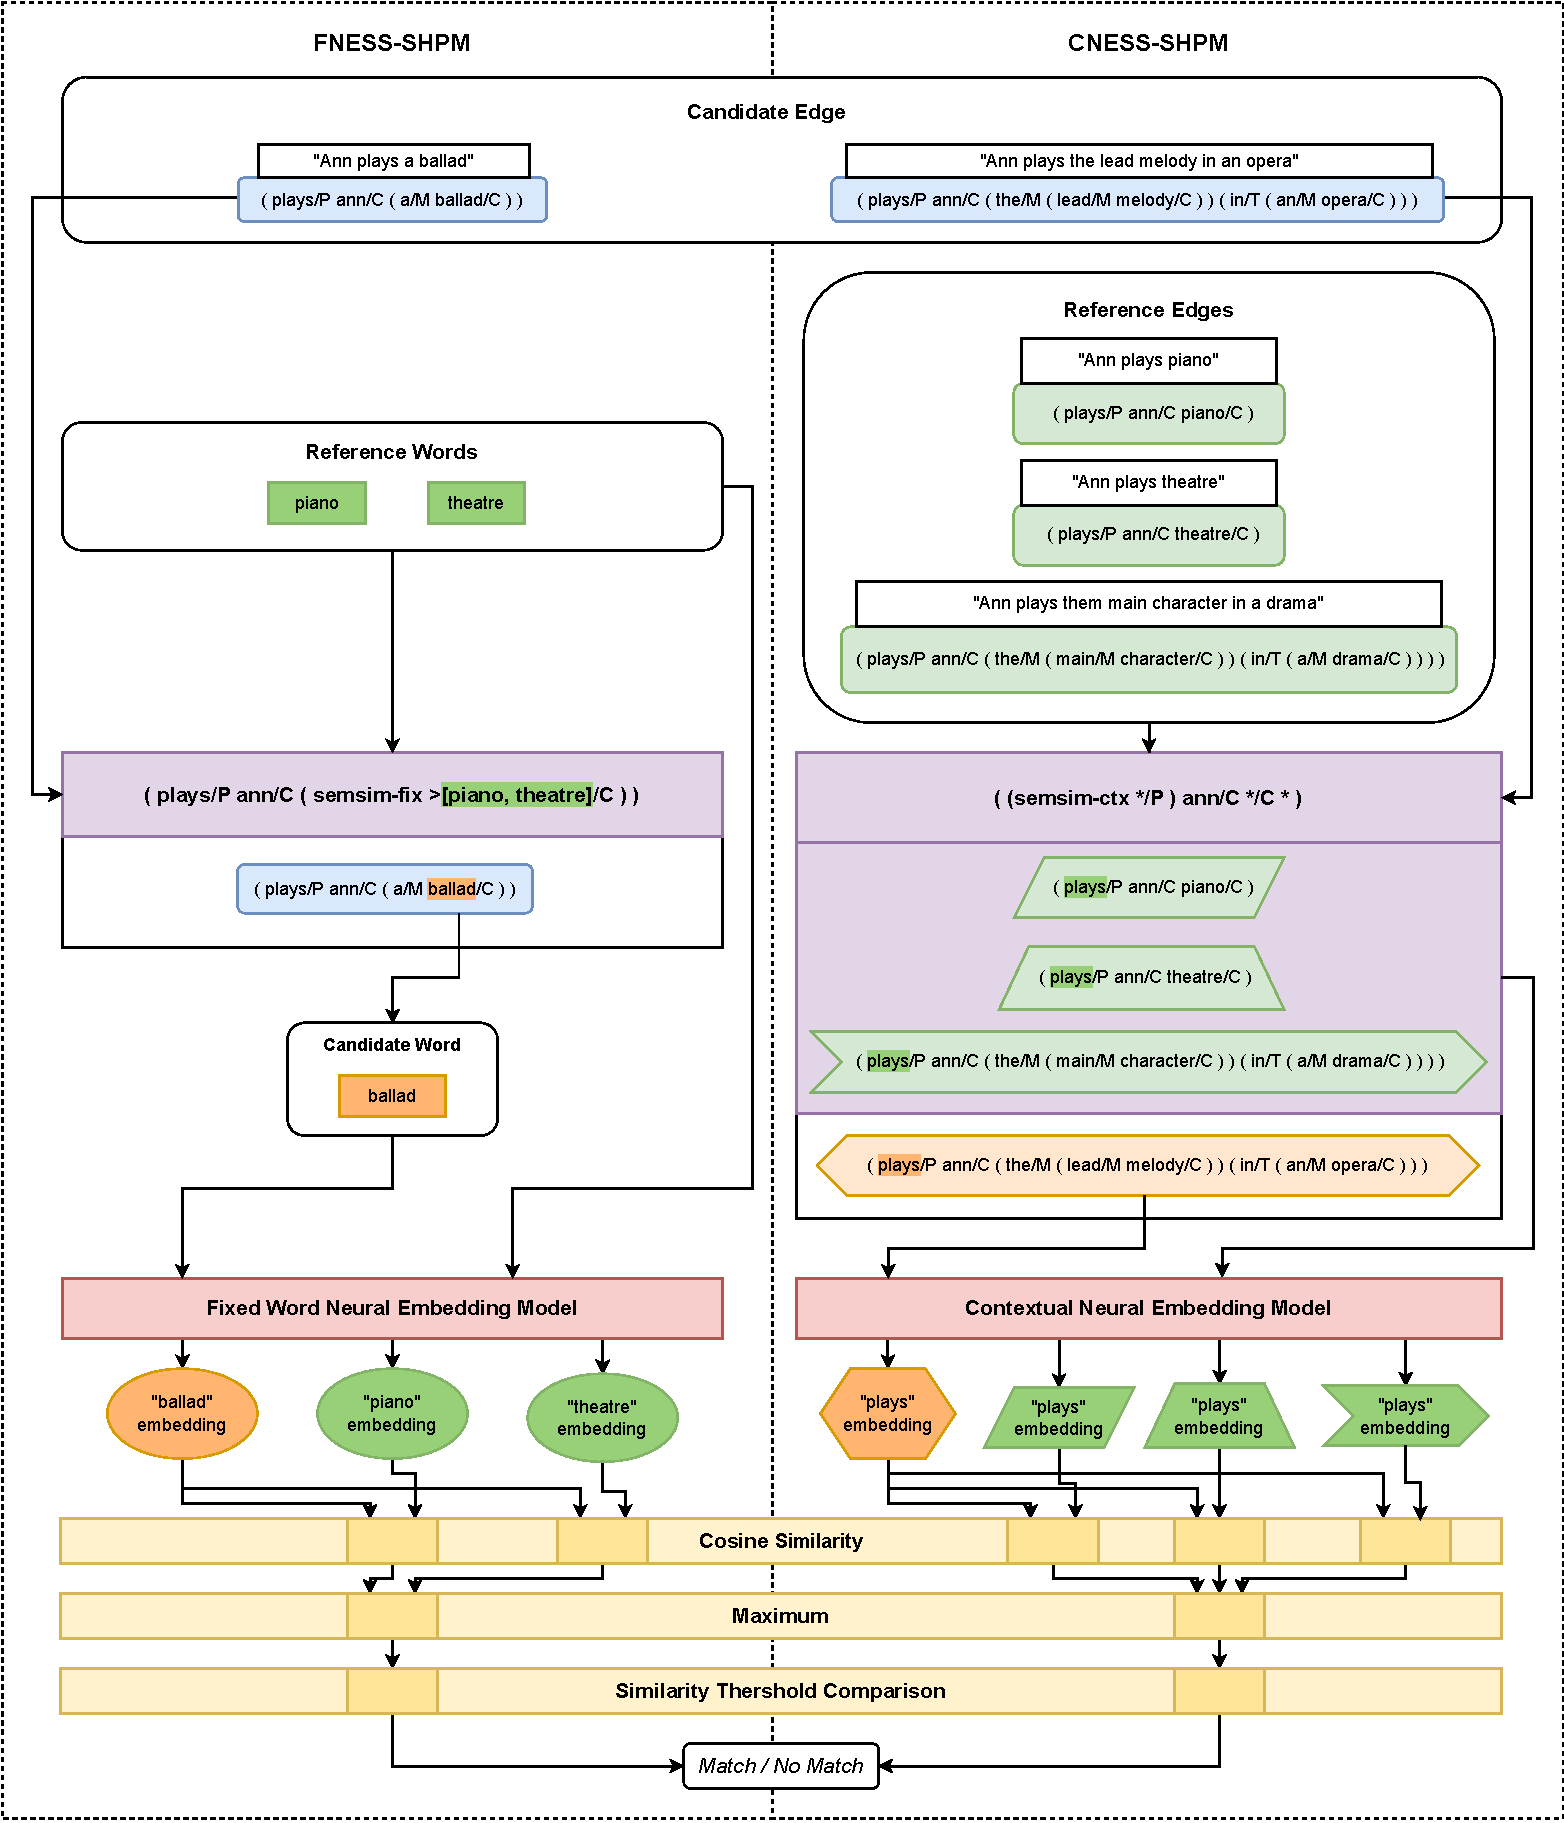
\includegraphics[width=\textwidth]{diagrams/concept-diagram.pdf}
\caption{Visualisation of the structure of both \gls{ness-shpm} variants, each matching a candidate edge against a pattern. Left side depicts \gls{fness-shpm}, while the right side illustrates \gls{cness-shpm}.}
% , as well as the SemSim instance post-processing}
\label{fig:concept-diagram}
\end{figure}


%\newpage

\subsection{Extention of the Pattern Language}
\label{sec:extension-pattern-language}
For the inclusion of \gls{ness}-based content matching within the \gls{sh} pattern language, the \textit{SemSim} functional pattern will be introduced. This addition is targeted at the functional pattern segment of the language, which is already predisposed to support flexible enhancements for \gls{sh} pattern matching. This approach is consistent with the existing mechanism of realising lemma-based content matching generalisation capabilities in the framework.


\subsubsection{SemSim Functional Pattern}
When constructing a \gls{sh} pattern that should be matched against a hypergraph, the \textit{SemSim} functional pattern can be utilised at those points in the pattern, where content should be matched by \gls{ness}. The added SemSim functional pattern -- also referred to as SemSim pattern -- has one of two syntactical structures: One that does include a variable and one that does not. 
Both variants of the SemSim pattern and examples of their usage are illustrated in the \cref{tab:semsim-pattern}. The SemSim pattern consists of different syntactical components, represented by placeholders that are enclosed in brackets (\texttt{<>}). These components are explained in detail below. Examples usages of SemSim patterns as sub-pattern inside other patterns are shown below the syntax component explanations.

\begin{table*}[h!]
\centering
\normalfont\sffamily
\setlength{\tabcolsep}{0pt}
\begin{tabular}{c@{\hspace{20pt}}ccccccccc}
\toprule
\textrm{No Variable}   & \texttt{<SF>} & \texttt{<IA>} & \texttt{<RC>} & \texttt{/} & \texttt{<HT>} & \texttt{.} & \texttt{<AR>} &  & \texttt{<ST>} \\
\midrule
\multirow{5}{*}{}
 & semsim-fix & & piano & / & C &  &   & & \\
 & semsim-fix & > & piano & / & C &  &   & & \\
 & semsim-fix & & piano & / & C & . & so & & \\
 & semsim-fix & & [piano, theatre] & / & C &  &   & & \\
 & semsim-fix & & piano & / & C &  &   & & 0.5 \\
 & semsim-fix & > & [piano, theatre] & / & C & . & so & & 0.5 \\
 & semsim-fix-lemma & > & [piano, theatre] & / & C & . & so & & 0.5 \\
 & semsim-ctx &  & * & / & C & . & so & & 0.5 \\
\midrule
\midrule
\textrm{With Variable} & \texttt{<SF>} & \texttt{<IA>} & \texttt{<VA>} & \texttt{/} & \texttt{<HT>} & \texttt{.} & \texttt{<AR>} & \texttt{<RC>} & \texttt{<ST>} \\
\midrule
 & semsim-fix & > & ART & / & C & . & so & [piano, theatre] & 0.5\\
 & semsim-fix-lemma & > & ART & / & C & . & so & [piano, theatre] & 0.5\\
 & semsim-ctx &  & ART & / & C & . & so & * & 0.5 \\
\bottomrule
\end{tabular}
\caption{
Syntactical structure of SemSim Pattern with specific examples.\\
Syntactical components: SemSim Function (\texttt{SF}), Reference Content (\texttt{RC}),  Variable Declaration (\texttt{VA}), Hyperedge Type (\texttt{HT}), Argument Roles (\texttt{AR}), Innermost Atom Operator (\texttt{IA}), Similarity Threshold (\texttt{\gls{st}})
}
\label{tab:semsim-pattern}
\end{table*}


%\subsubsection{SemSim Function (\texttt{SF})}
\paragraph{SemSim Function (\texttt{SF})}
 The semsim function can be one of the following: \texttt{semsim-fix}, \texttt{semsim-fix-lemma} and \texttt{semsim-ctx}. These functions correspond to fixed word neural embedding-based, lemma-based fixed word neural embedding-based and contextual neural embedding-based semantic similarity measurement.

%\subsubsection{Reference Content (\texttt{RC})} 
\paragraph{Reference Content (\texttt{RC})} 
The reference content is used to specify the reference word(s) for the \gls{fness} variant. The square bracket notation which is already part of the \gls{sh} pattern language is leveraged to pass multiple words as a list. The reference edge(s) that is needed for the contextual \gls{ness} variant is not given via the semsim functional pattern itself, but as a software interface argument to the matching process due to practical considerations (see \cref{sec:pl-extension-limitations}).


\paragraph{Variable Declaration (\texttt{VA})} 
If the content of the sub-edge captured by the SemSim sub-pattern should be captured in a variable, the second variant of the syntax applies. This notation is in line with the usage of the lemma functional pattern illustrated in \cref{sec:sh-pattern-matching}.


%\subsubsection{Hyperedge Type (\texttt{HT}) and Argument Roles (\texttt{AR})}
\paragraph{Hyperedge Type (\texttt{HT}),  Argument Roles (\texttt{AR}) and Innermost Atom Operator (\texttt{IA})} These pattern components can be utilised in the same way as illustrated above in \cref{sec:sh-pattern-matching} for the lemma functional pattern.
Hyperedge type and argument roles are matched following the symbolic rules also described above. The innermost atom operator (\texttt{>}) can be placed in front of the reference content or the variable declaration if applicable.


%\subsubsection{Similarity Threshold (\texttt{\gls{st}})}
\paragraph{Similarity Threshold (\texttt{\gls{st}})}
%The similarity threshold used to decide whether candidate and reference content matched, given that the \gls{ness} measurement has already been computed. This applies to the fixed as well as to the contextual variant of \gls{ness}. 
The similarity threshold \(t_s\) can optionally be specified for a specific occurrence of the SemSim functional pattern, but it can also be given as a global parameter of the matching process (see \cref{sec:ness-config}). 

\subsubsection{Example Usages}
\label{sec:semsim-pattern-example-usages}

To illustrate the usage of the SemSim functional pattern as sub-pattern in another pattern, some examples are given below. We restrict these examples here to the \texttt{semsim-fix} pattern, since the \texttt{semsim-ctx} pattern additionally requires the definition of reference edges.

\begin{pattern}[h!]
  \normalfont\sffamily
  \centering
  ( plays/P ann/C (semsim-fix piano/C) )
  \caption{"Ann plays something similar to piano" pattern}
%  \label{pat:ann-likes-semsim-aplles}
\end{pattern}

\begin{pattern}[h!]
  \normalfont\sffamily
  \centering
  ( plays/P ann/C (semsim-fix [piano, theatre]/C) )
  \caption{"Ann plays something similar to piano or theatre" pattern}
%  \label{pat:ann-likes-apples-and-bananas}
\end{pattern}


\begin{pattern}[h!]
  \normalfont\sffamily
  \centering
  ( plays/P ann/C (semsim-fix theatre/C 0.5) )
  \caption{"Ann plays something similar to theatre" pattern with \(t_s = 0.5\)}
%  \label{pat:ann-likes-semsim-aplles}
\end{pattern}


\subsubsection{Limitations of the Pattern Language Extension}
\label{sec:pl-extension-limitations}
The utilisation of the fixed variant of \gls{ness-shpm} is possible solely via the SemSim functional pattern. This means that all information that is required to apply \gls{fness}-based content matching, specifically the reference content and the similarity threshold, can be included in a \gls{sh} pattern. In contrast, it was found impractical to provide the reference edges needed for the contextual \gls{ness} variant via a \gls{sh} pattern. While the reference content argument could generally be used for that, this would result in very exhaustive patterns and impair their readability for humans. Therefore the conceptual design choice was made to pass the reference edges via the software interface of the \gls{sh} pattern matching.


\subsection{Modification of the Pattern Language Processing}
\label{sec:modifications-pattern-language-processing}
This section outlines the integration of SemSim functional pattern processing with the current pattern language processing. The process is triggered when a pattern, incorporating a SemSim pattern, is matched against a specific hyperedge and the SemSim pattern is reached without any prior mismatches. At this point, the SemSim pattern captures a sub-edge for processing, which includes the symbolic structural matching. 
%of the hyperedge type and possibly argument, as well as the application of the innermost atom operator, if specified. 
Additionally the necessary information for \gls{ness} measurement computations is extracted.

The operation of SemSim pattern processing changes based on the specific SemSim function applied. With \gls{fness-shpm} or \gls{lfness-shpm}, the process extracts the candidate word(s) or their lemma(s) from the identified sub-edge and the reference word(s) from the pattern. This extraction process requires the sub-edge to be atomic, which implies combination with the innermost atom operator to ensure functionality in all cases. For \gls{cness}, it conducts a standard string-based matching of the reference content. Therefore  utilizing the wildcard operator as a reference content argument is sensible in most practical use cases. For any \gls{ness-shpm} variant, the similarity threshold is extracted from the SemSim pattern, if given.

Existing components manage the symbolic matching of hyperedge type and argument roles, as well as the application of the innermost atom operator, consistent with the standard pattern matching. The SemSim function, along with the similarity threshold (when provided), candidate words and reference words for (L)\gls{fness-shpm}, are passed to the newly designed \gls{ness} computation components.


%\subsection{\gls{ness} Measurement Computations}
%When the \gls{ness-shpm} process arrives at this point, the candidate and reference contents have either been extracted by the pattern language processing (in case of \gls{fness-shpm}M) or passed down as software interface arguments (in the case of \gls{cness-shpm}). The similarity threshold has either also been extracted from the SemSim pattern or was given to the \gls{ness-shpm} process as a global default parameter via the software interface. So now the candidate and reference content can be used go to obtain the respective embeddings used to perform the similarity measurement between them.
%
%\todo{How it the \gls{ness} model specified? talk about ness config?}
%
%\subsubsection{Fixed Neural Embeddings}
%To generate the fixed neural embeddings, only the candidate word(s) and the reference word(s) are needed. Since every word corresponds to a fixed embedding, a simple lookup is performed using the specified fixed neural embedding model to generate the candidate and reference embeddings.
%
%\subsubsection{Contextual Neural Embeddings}
%The construction of the contextual candidate and reference embeddings involves multiple steps. It is assumed that the embeddings should correspond to the sub-edge captured by the SemSim pattern and their counterparts in the reference edges. Thereby the reference edges need to structurally match (with no regard to edge content) the pattern which contains the SemSim functional pattern, so that these reference sub-edges can be identified. To enable verification of this assumption another version of the contextual neural embedding construction is conceptualised, which omits the sub-edge correspondence of the embeddings. For this version only the first two steps of the following construction process are relevant.
%
%\begin{enumerate}
%	\item Reconstruction of the phrases or sentences (context items) from the candidate and reference edges.
%	\item Generating the embeddings for the candidate and reference context items using the specified contextual neural embedding model.
%	\item Identification of the sub-edge in the reference edges that corresponds to the sub-edge in the candidate edge, which was captured by the SemSim functional pattern.
%	\item Mapping of the candidate and reference sub-edge to the relevant sub-embeddings of the candidate and reference context item embeddings.
%	\item Generation of the actual candidate and reference embeddings based on these candidate and reference sub-embeddings.
%\end{enumerate} 
%
%
%\subsubsection{Embedding Similarity Measurement}
%The cosine similarity between the candidate and reference embeddings is computed and compared to the given similarity threshold. If the computed similarity is greater than the threshold, the candidate and reference content are considered to match. 


\subsection{Neural Embedding-based Semantic Similarity Measurement}
\label{sec:neural-embedding-based-semantic-similarity-measurement}
Upon reaching this phase, the \gls{ness-shpm} process has already either extracted candidate and reference contents via pattern language processing (in case of \gls{fness-shpm}) or received them through software interface arguments (in case of \gls{cness-shpm}). Similarly, the similarity threshold has been either derived from the SemSim pattern or assigned as a default parameter through the software interface. Additionally the \textit{\gls{ness} type} (i.e \gls{fness} or \gls{cness}) is determined by the SemSim function and a specific \textit{\gls{ness} model} (i.e. neural embedding model) has been specified through the software interface. Consequently, the process is set to obtain the respective embeddings for the candidate and reference content, which are central for conducting the semantic similarity assessment.

We denote the arguments of the NESS measurement (\(A_\text{NESS}\)) as follows:
Pattern \(p\), candidate content \(c_\text{can}\), reference content(s) \(C_\text{ref}\) and similarity threshold \(t_s\). The candidate content is either a candidate word \(w_\text{can}\) or a candidate edge \(e_\text{can}\). The reference content is either a set of reference words \(W_\text{ref}\) or a set of reference edges \(E_\text{ref}\). The similarity threshold is either extracted from the pattern \(t_{s_\text{pat}}\) or given as a default parameter \(t_{s_\text{def}}\).

\[
A_\text{NESS} = \{p, c_\text{can}, C_\text{ref}, t_s\}
\]
\[
c_\text{can} \in \{w_\text{can}, e_\text{can}\} \ ,\ C_\text{ref} \in \{W_\text{ref}, E_\text{ref}\} \ ,\ W_\text{ref} = \{w_0, \dots, w_n\}, E_\text{ref} = \{e_0, \dots, e_m\} \ ,\ n,m \in \mathbb{N}^+
\]
\[
C_\text{ref} = 
\begin{cases} 
W_\text{ref} & \text{if } c_\text{can} = w_\text{can}, \\
E_\text{ref} & \text{if } c_\text{can} = e_\text{can}.
\end{cases}
\]
\[
t_s \in \{t_{s_\text{pat}}, t_{s_\text{def}}\}
\]

\subsubsection{Fixed Neural Embeddings}
The creation of fixed neural embeddings necessitates only the candidate and reference words. Given that each word maps directly to a specific embedding, a straightforward lookup in the chosen fixed neural embedding model suffices to produce the necessary embeddings for both candidate and reference. The embedding \(v_w\) of word \(w\), generated by fixed word neural embedding model \(M_\text{fix}\) is denoted as:

\[v_w = M_\text{fix}(w),\ V_W = \{v_w\ |\ w \in W\} \]

\subsubsection{Contextual Neural Embeddings}
The construction of contextual embeddings for the candidate and reference content involves a sequence of steps, premised on the assumption that these embeddings should mirror the specific sub-edge of the candidate edge captured by the SemSim pattern and its analogous sub-edge(s) in the reference edge(s). Thereby the reference edges need to structurally match (with disregard to edge content) the pattern, which contains the SemSim functional pattern, so that these reference sub-edges can be identified. 

An alternative approach to constructing contextual neural embeddings does not account for sub-edge matching and only consists of the initial two stages of the construction process outlined below. This variant of the contextual embedding construction is in the following referred to as the \gls{at} option.

\begin{enumerate}
	\item Reconstructing phrases or sentences from the candidate and reference edges (deemed context items).
    \item Producing embeddings for these context items using the designated contextual neural embedding model.
    \item Identifying the sub-edge within the reference that aligns with the candidate's sub-edge captured by the SemSim pattern.
    \item Associating the identified candidate and reference sub-edges with their respective sub-embeddings derived from the context item embeddings.
    \item Generating the final embeddings for both candidate and reference based on these sub-embeddings.
\end{enumerate}

The embedding \(v_e\) of edge \(e\), generated by the contextual neural embedding model \(M_\text{ctx}\) when considering pattern \(p\), is denoted as:


\[v_e = M_\text{ctx}(e, p),\ V_E = \{v_e\ |\ e \in E\} \]

    
\subsubsection{Embedding Similarity Measurement}
The procedure calculates the cosine similarity between the embeddings of candidate and reference content, comparing it to the pre-established similarity threshold. If the resultant similarity score surpasses this threshold, the candidate and reference contents are considered to match. Given multiple reference content items (and therefore multiple reference embeddings), the pairwise cosine similarities between the candidate and the reference embedding is computed. The maximum of these similarities is then compared to the similarity threshold to asses whether the candidate and reference contents match. Semantic similarity \(f_\text{semsim}\) given the arguments \(A_\text{NESS} = \{p, c_\text{can}, C_\text{ref}, t_s\}\) is therefore calculated by:

%\[f_\text{semsim}(A_e) = max(\{cos_\text{sim}(M(c_\text{can}, p^*), M(c_\text{ref}, p^*))\ |\ c_\text{ref} \in C_\text{ref}\}) \geq t_s \]
\[f_\text{semsim}(A) = max(\{cos_\text{sim}(v_\text{can}, v_\text{ref})\ |\ v_\text{ref} \in V_\text{ref} \}) \geq t_s  \]
\[
V_\text{ref} = 
\begin{cases} 
V_{W_\text{ref}} & \text{if } v_\text{can} = v_{w_\text{can}}, \\
V_{E_\text{ref}} & \text{if } v_\text{can} = v_{e_\text{can}}.
\end{cases}
\]

%\[M \in \{M_\text{fix}, M_\text{ctx}\},\ \text{if}\ M = M_\text{fix}\ \text{then}\ p^* = \varnothing,\ \text{if}\ M = M_\text{ctx}\ \text{then}\ p^* = p \]

Cosine similarity is chosen as spatial measure, since it has been show well suited for assessing semantic similarity in vector spaces (see \cref{sec:corpus-based-semantic-similarity}) and is an established measure in the context of neural text embeddings (see \cref{sec:neural-embedding-semantic-similarity}). The maximum of the pairwise similarities is used for comparison with the similarity threshold, because in case of FNESS, we want the reference words always to be deemed semantically similar to themselves. This would not necessarily be the case when using e.g. the mean of the pairwise similarities. However, other methods such as e.g a weighted mean could principally also be of interest, especially for CNESS.




% ========== 
\chapter{Implementation}
\label{cha:implementation}
\glsreset{ness-shpm}

In this chapter we will present and explain the implementation of the solution approach conceived in \cref{cha:solution-approach}, which takes the form of a software realisation of \gls{ness-shpm}.

The entailing software design and development is centred around integrating the necessary functionality in the existing publicly available software package \textit{graphbrain}\footnote{graphbrain: \url{https://graphbrain.net/}}, which includes an implementation of the Semantic Hypergraph framework. This integration consists of two primary aspects: Modifying and augmenting the existing pattern language processing components to accommodate the extended pattern language (confer \cref{sec:extension-pattern-language} and \cref{sec:modifications-pattern-language-processing}), as well as constructing new software components to realise the \gls{ness} measurement (confer \cref{sec:neural-embedding-based-semantic-similarity-measurement}).

Implementation details, which are considered not to contribute to the general understanding of the software system, are omitted or  have been modified for better readability and clarity. This means that all code listing presented below are pseudocode.



\section{Overview of \textit{graphbrain}}
This section offers a concise overview of the essential elements of the graphbrain package, detailing its software architecture. It also describes specific aspects of the hypergraph data structure and the \gls{nl} to \gls{sh} parsing procedure that are of peripheral relevance here.

The graphbrain package contains the \texttt{graphbrain} Python module, which consists of several submodules. The architecture of the key parts of the modified and extened \texttt{graphbrain} module is depicted in \cref{fig:graphbrain-architecture}. This diagram highlights the primary call chain and data flow involved in the pattern matching process, while the return chain is excluded to enhance the diagram's clarity. Further details on the software structure and procedural flow are elaborated in subsequent sections.

Here, we focus on two particular submodules: the \texttt{graphbrain.patterns} submodule, which is primarily responsible for the pattern matching process and has therefore been significantly modified and expanded, and the newly created \texttt{graphbrain.semsim} submodule, which hosts the implementations of \gls{ness} measurements. 

Of secondary importance are the \texttt{graphbrain.hypergraph} and \texttt{graphbrain.hyperedge} submodules, which are responsible for implementing the structures of the hypergraph and hyperedge, respectively.

\begin{figure}
\centering
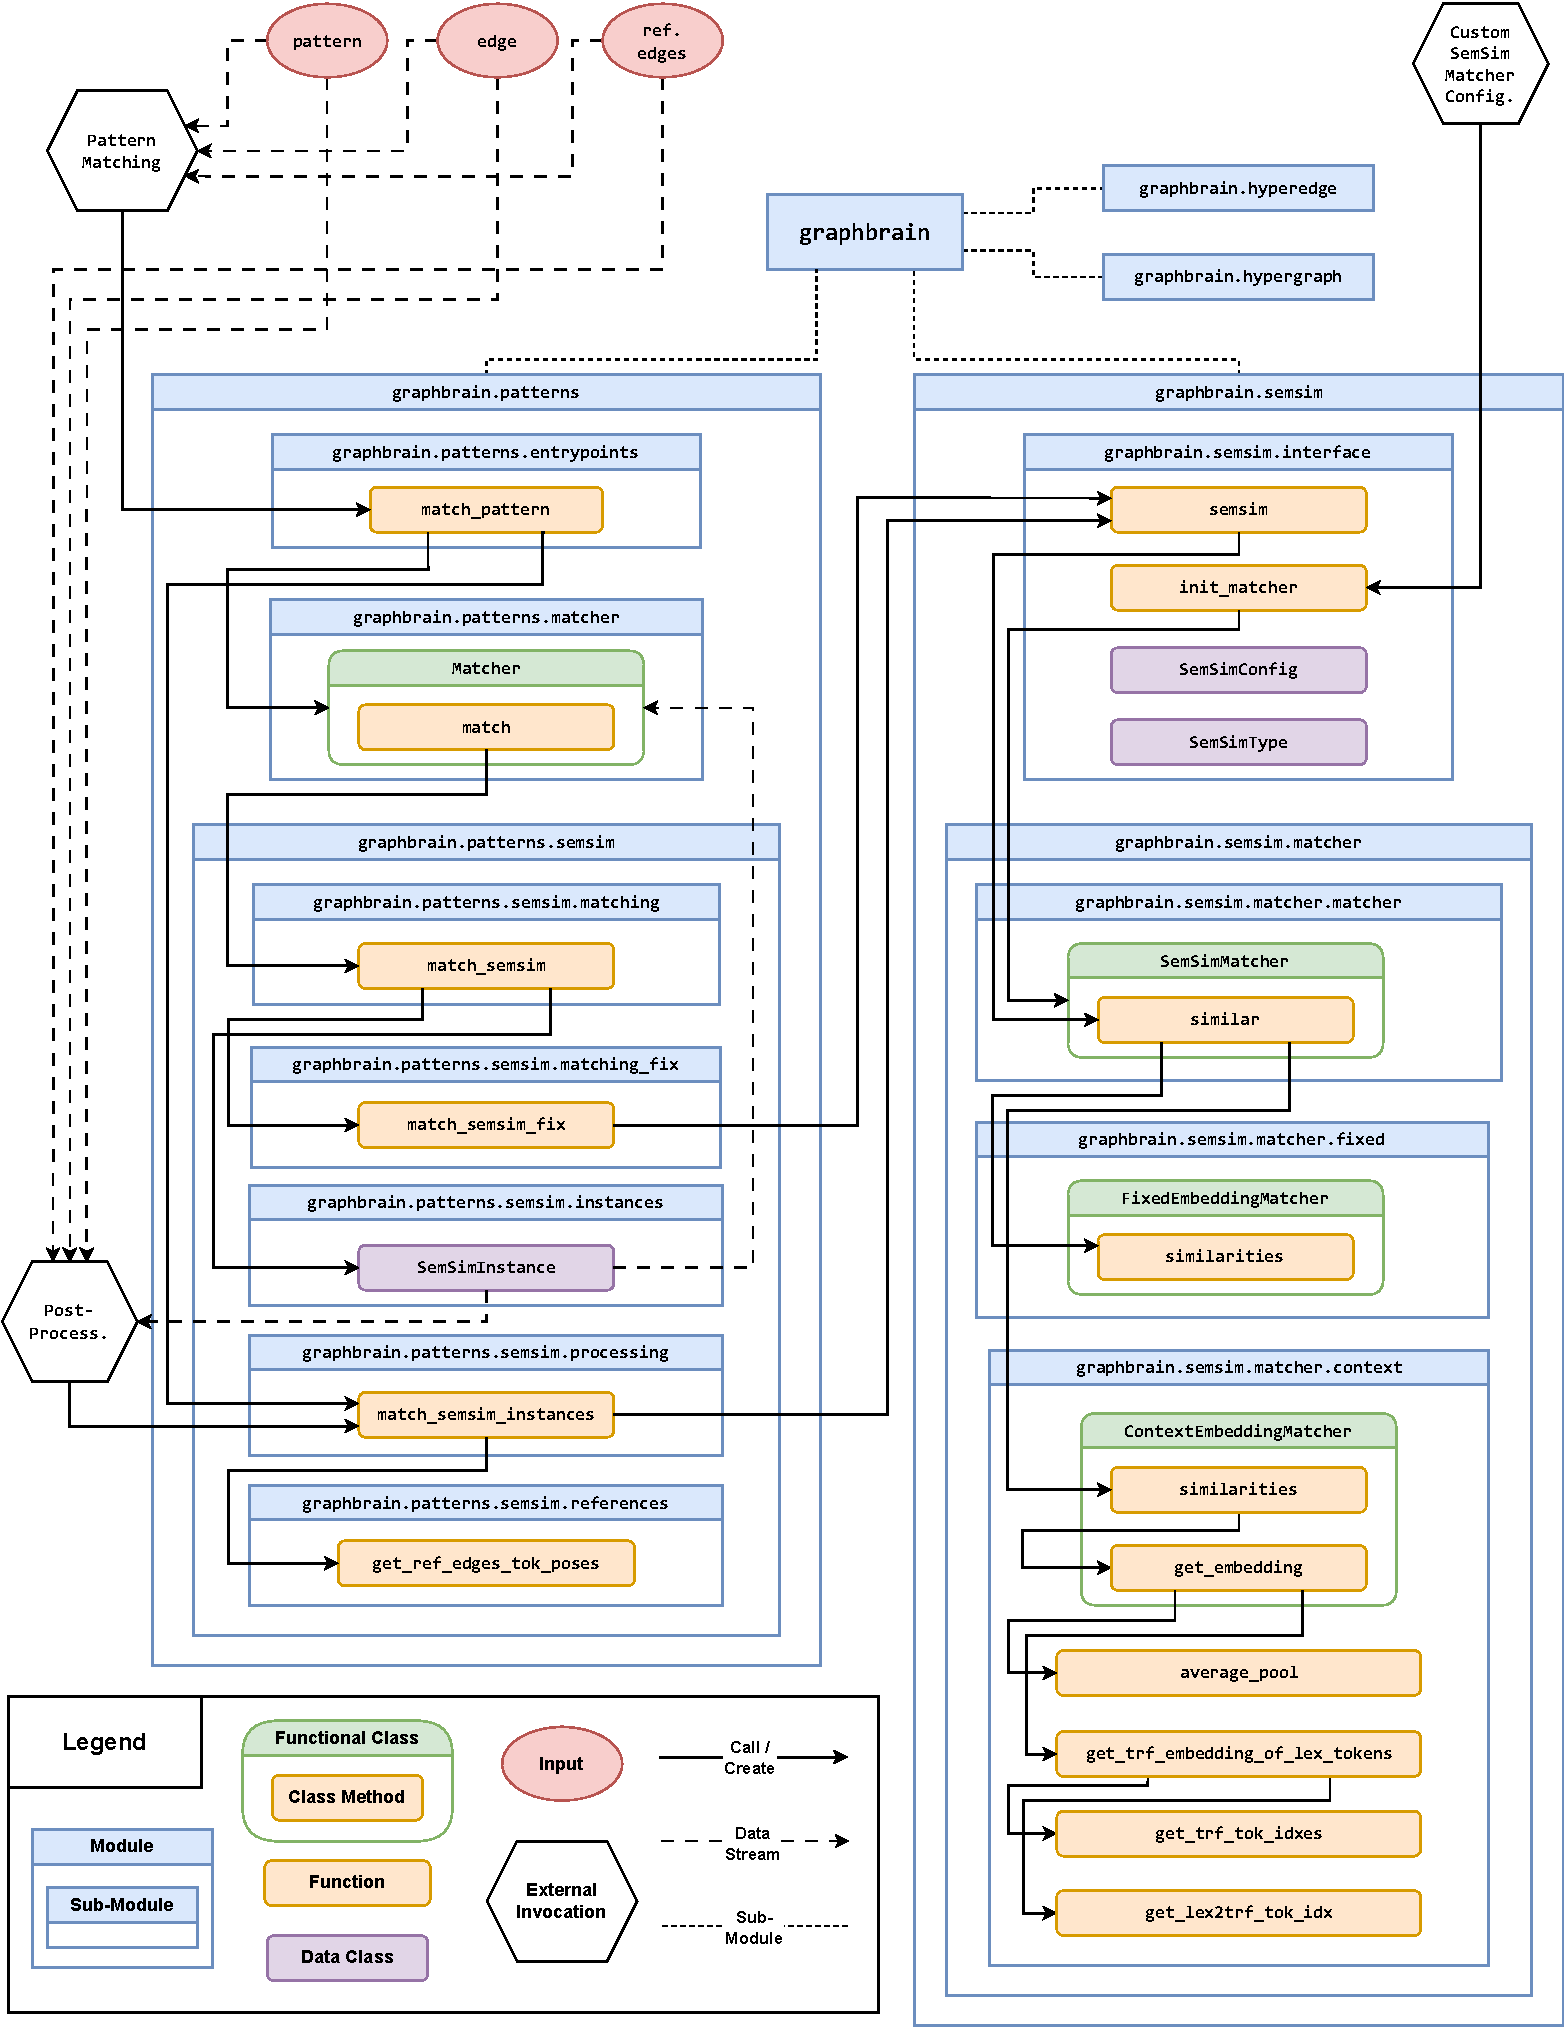
\includegraphics[width=\textwidth]{diagrams/graphbrain-architecture.pdf}
\caption{Simplified architecture diagram of the modified and extended \texttt{graphbrain} Python module, with primary call chain and data stream for the pattern matching process (return chain is omitted for visual clarity).}
% , as well as the SemSim instance post-processing}
\label{fig:graphbrain-architecture}
\end{figure}


\subsubsection{Hypergraph Implementation}
A specific hypergraph is implemented in form of a key-value storage, for which currently \textit{LevelDB}\footnote{LevelDB: \url{https://github.com/google/leveldb}} and \textit{SQLite}\footnote{SQLite: \url{https://www.sqlite.org/}} are support as database backends. Interfaces for the key-value storages are implemented in \texttt{graphbrain.memory}. However, details of this implementation are irrelevant for this work.


\subsubsection{\gls{nl} to \gls{sh} Parser Implementation}
\label{sec:nl-to-sh-parser-implementation}
The translation process from natural language to the Semantic Hypergraph representations (see \cref{sec:sh-translation-process}), depends significantly on the established NLP library \textit{spaCy} \cite{honnibal2020spacy}. Although the translation itself holds limited relevance for this work, it is important to note that the atomic edges in a \gls{sh} representation of a sentence closely relate to the tokens resulting from the tokenisation of this sentence by spaCy's lexical tokeniser.\footnote{spaCy Lexical Tokeniser: \url{https://spacy.io/usage/linguistic-features\#tokenization}}


%Differences between \gls{sh} Formalism and graphbrain
%
%Some features of the \gls{sh} Pattern Language and therefore the \gls{sh} Pattern Matching Process are implemented differently in graphbrain then they are defined in the pattern language.
%Specifically variables, options list and the innermost atom operator are implemented in graphbrain in the form of functional patterns. These requires a slightly different syntax for patterns to be processable by graphbrain, than would be valid in the formal \gls{sh} pattern language.
%
%--> is this actually relevant, if i only use formal patterns in the evaluation chapter?
%--> does not hurt to mention it, but only relevant if it comes up later


\section{Pattern Processing: \texttt{graphbrain.patterns}}
The \texttt{patterns} module has been restructured from a monolithic design into multiple submodules to facilitate implementing the necessary modifications to the pattern language processing (see \cref{sec:modifications-pattern-language-processing}), which are required to support the extended pattern language (see \cref{sec:extension-pattern-language}). This includes the creation of the \texttt{patterns.semsim} submodule. Furthermore, some adjustments to the software architecture have been made to simplify the implementation of contextual \gls{ness} extended pattern matching (see \cref{sec:graphbrain.patterns.matcher}). Apart of the SemSim-specific submodule, the \texttt{patterns.entrypoints} and \texttt{patterns.matcher} submodules are also of relevance for this work.

Some general intricacies of the implementation \gls{ness} extended Semantic Hypergraph pattern matching are discussed below, before the specific implementation in the aforementioned submodules is presented.


\subsubsection{In-Line- vs. Post-Processing}
While the processing of the SemSim functional pattern in the sense of pattern language processing always needs to happen in-line with the regular pattern matching, the actual \gls{ness} computations may happen as a post-processing step. When the pattern matching process arrives at a SemSim functional pattern, the symbolic part of the SemSim pattern -- i.e. the hyperedge type and the argument roles -- are processed immediately, hence in-line. In the case of the contextual variant, the \gls{cness} computations always occur as a post-process. This means that for a given combination of edge and pattern -- in which the latter contains at least one occurrence of a \texttt{semsim-ctx} sub-pattern --  the entire edge and pattern are first matched in regards to everything else. The information necessary for the \gls{cness} measurement is recorded at this point and the actual computations take place afterwards, if everything else matched. This design choice has two advantages: Firstly, the context information does not have to be passed down to the SemSim functional pattern matching step and secondly, the computationally expensive \gls{cness} measurements can be avoided, if unnecessary.

\subsubsection{SemSim Instances and SemSim Skipping}
The recording of the information needed for \gls{ness} measurements takes the form of \textit{SemSim Instances}, which can then processed mostly independent from the \gls{sh} pattern matching.  
It is possible to configure the pattern matching process via a \textit{SemSim Skipping} option of its software interface, such that the \gls{ness} computations are skipped entirely. In this case -- also for \texttt{semsim-fix} sub-patterns -- only the symbolical matching takes place in-line and the SemSim Instances are returned alongside the symbolic matching results. With the skipping option disabled, the \texttt{semsim-ctx} related instances are still post-processed as part of the pattern matching process. Isolating the \gls{ness} computation by enabling SemSim skipping is especially useful, if the \gls{ness} measurements shall be computed with a set of different \gls{ness} configuration parameters (e.g. different similarity thresholds), for example in an experimental evaluation.

\subsubsection{Token Position Passing}
To enable the contextual \gls{ness} measurement computations, the \textit{Token Position} has to be provided. In this work, this describes a data structure containing the positions of the tokens corresponding to atoms in a hyperedge. Position here refers to the index of a token in the token sequence, that resulted from the tokenisation of a sentence, when it was translated into a hyperedge (see \cref{sec:nl-to-sh-parser-implementation}). An example of a tokenised sentence with its corresponding hyperedge and token position is given in \cref{tab:example-token-position}. 
The structure of a token position follows the same structure as the hyperedge, which means the token position can be seen as a hyperedge itself (and it is implemented this way). The hypergraph data structure was extended, such that every root edge has an attribute that stores its token position. For the \gls{cness} measurements it is necessary to identify which tokens correspond to the sub-edge that is captured by \texttt{semsim-ctx} sub-pattern. Therefore, the token position is passed down alongside the recursive matching process, such that the corresponding sub token position and therefore the relevant token indices can be recorded. 


\begin{table}
\centering
\begin{tabular}{lccccccc}

\textbf{Tokenised Sentence} &	  & jerome & eats &  & an & apple & \\
\textbf{Token Indices} &	  & 0	& 1 & & 2 & 3 & \\

	  \midrule

\textbf{Hyperedge} &	  ( & \textsf{eats/P} & \textsf{jerome/C} & ( & \textsf{an/M}  & \textsf{apple/C} & ) ) \\
\textbf{Token Position} & 	  ( & 1 & 0 & ( & 2 & 3 & ) )
\end{tabular}	
\caption{Example of a token position}
\label{tab:example-token-position}
\end{table}

 
\subsection{Entry-Point and Pattern Matcher} 
 
\subsubsection{\texttt{graphbrain.patterns.entrypoints}}
\label{sec:graphbrain.patterns.entrypoints}
This module contains all entry-points for pattern matching, primarily serving the hypergraph class. The central entry-point is the \texttt{match\_pattern} method (see \cref{psd:match-pattern-function}), which matches a pattern against an edge. This method incorporates a \texttt{skip\_semsim} argument to control SemSim skipping. A new \texttt{Matcher} object (see \cref{sec:graphbrain.patterns.matcher}) is constructed for every matching procedure (i.e pattern-edge pair). This object maintains the results of the symbolic pattern matching or \gls{fness} extended pattern matching, as well as the SemSim instances that may have been recored due to \gls{cness} extended pattern matching or enabled SemSim skipping. After successful symbolic matching, the \texttt{match\_semsim\_instances} function (see \cref{sec:graphbrain.patterns.semsim.processing}) is called from here, if SemSim skipping is disabled. 

%when the pattern features a \texttt{semsim-fix} sub-pattern. Moreover, the \texttt{Matcher} object may record SemSim instances if the pattern encompasses a \texttt{semsim-ctx} sub-pattern. 
%In case the \texttt{skip\_semsim} argument is activated, SemSim instances are always recored and returned, if the edge matches the pattern structurally and it involves any \texttt{semsim} sub-pattern.


\begin{pseudo}
\begin{lstlisting}
def match_pattern(edge, pattern, ref_edges, skip_semsim, hypergraph):
    matcher: Matcher = Matcher(
        edge, pattern, skip_semsim, hypergraph
    )

    if skip_semsim:
        return matcher.results, matcher.semsim_instances

    if matcher.results and match_semsim_instances(
            matcher.semsim_instances,
            pattern,
            edge,
            ref_edges,
            hypergraph
    ):
        return matcher.results

    return []
\end{lstlisting}
\caption{\texttt{match\_pattern} function}
\label{psd:match-pattern-function}
\end{pseudo}



\subsubsection{\texttt{graphbrain.patterns.matcher}}
\label{sec:graphbrain.patterns.matcher}
This module contains the newly created \texttt{Matcher} class (see \cref{psd:matcher-class}), designed to function as a stateful object, facilitating the implementation of \gls{cness} extend pattern matching. This object records the symbolic matching results and SemSim instances in its \texttt{Matcher.results} and \texttt{Matcher.semsim\_instances} attributes respectively. It also has an \texttt{Matcher.skip\_semsim} and a \texttt{Matcher.hg} (hypergraph) attribute that store the passed argument values. The classes functionality is primarily realised in the \texttt{Matcher.match} method, which serves as the pattern matching recursion entry-point. From this method the \texttt{match\_semsim} function is called, if a SemSim pattern is encountered.


\begin{pseudo}
\begin{lstlisting}
class Matcher:
    def __init__(self, edge pattern, skip_semsim, hypergraph):
        self.hg = hypergraph
        self.skip_semsim = skip_semsim

        self.semsim_instances = []
        self.results = self.match(
            edge, pattern, current_results=[], tok_pos=get_tok_pos(edge)
        )
\end{lstlisting}
\caption{Pattern \texttt{Matcher} class}
\label{psd:matcher-class}
\end{pseudo}


\subsection{SemSim Pattern In-Line Processing}
The processing of the SemSim functional patterns that occurs in-line with the symbolic matching is implemented in the following submodules of the \texttt{patterns.semsim} module:


\subsubsection{\texttt{graphbrain.patterns.semsim.matching}}
This module contains the \texttt{match\_semsim} function (see \cref{psd:match-semsim-function}) which is called by a \texttt{Matcher} object. In case of \gls{fness} extended pattern matching, the \texttt{match\_semsim\_fix} function (see \cref{sec:graphbrain.patterns.semsim.matchingfix}) is called -- also if SemSim skipping is enabled -- to extract the candidate word form the sub-edge and perform the matching with the structural symbolic part of the \texttt{semsim-fix} pattern. For \gls{cness} extended pattern matching the pattern is matched symbolically. If the applicable operation of these two returns a \textit{Match}, then a SemSim instance is recorded by the matcher in the case of \gls{cness} extended pattern matching or enabled SemSim skipping.

\begin{pseudo}
\begin{lstlisting}
def match_semsim(
    matcher, semsim_function, pattern, edge, current_results, tok_pos
):
    semsim_type, semsim_fix_use_lemma = get_semsim_type(semsim_fun)
    similarity_threshold = extract_similarity_threshold(pattern)

    results = []
    candidate_word = None   

    if semsim_type == SemSimType.FIX:
        semsim_fix_results, candidate_word = match_semsim_fix(
            pattern,
            edge,
            current_results,
            matcher.skip_semsim,
            semsim_fix_use_lemma,
            similarity_threshold,
            hypergraph
        )
        if semsim_fix_results is not None:
            results = semsim_fix_results

    if semsim_type == SemSimType.CTX:
        results = matcher.match(edge pattern, current_results, tok_pos)

    if results and (matcher.skip_semsim or semsim_type == SemSimType.CTX):
        add_semsim_instance(
            matcher, 
            semsim_type, 
            edge, 
            candidate_word, 
            tok_pos, 
            similarity_threshold
        )

    return results
\end{lstlisting}
\caption{\texttt{match\_semsim} function}
\label{psd:match-semsim-function}
\end{pseudo}


\subsubsection{\texttt{graphbrain.patterns.semsim.matching\_fix}}
\label{sec:graphbrain.patterns.semsim.matchingfix}
This module contains the \texttt{match\_semsim\_fix} function (see \cref{psd:match-semsim-fix-function}) which is called by the \texttt{match\_semsim} function.
The method first tries to extract the candidate word from the edge, which requires it to be an atom. If the extraction fails, because the edge is not atomic, it is considered not to match. Otherwise, a modified version of the pattern is created, where the pattern content is replaced by the wildcard operator. This modified pattern is then matched against the atomic edge to check if matches structurally (i.e regarding hyperedge type and argument roles). If this is the case and SemSim skipping is disabled, the reference words are extracted from the pattern and the \texttt{semsim} function is called, which is the entry-point to the actual \gls{ness} measurement implementation.

\begin{pseudo}
\begin{lstlisting}
def match_semsim_fix(
    pattern, edge, current_results, skip_semsim, use_lemma, threshold, hg,
):
    candidate_word = get_candidate_word(edge, use_lemma, hg)
    if not candidate_word:
        return None, None

    pattern_with_wildcard_content = replace_pattern_content(pattern, '*')
    if not matches_atomic_pattern(edge, pattern_with_wildcard_content):
        return [], None

    if not skip_semsim:
        reference_words = extract_reference_words(pattern)

        if not semsim(
            semsim_type=SemSimType.FIX,
            threshold=threshold,
            cand_word=candidate_word,
            ref_words=reference_words,
        ):
            return [], candidate_word

    return [current_results], candidate_word
 
\end{lstlisting}
\caption{\texttt{match\_semsim\_fix} function}
\label{psd:match-semsim-fix-function}
\end{pseudo}

\subsection{SemSim Instance Post-Processing}
The post-processing of SemSim instances is realised in the following submodules:

\subsubsection{\texttt{graphbrain.patterns.semsim.instances}}

This module primarily defines the \texttt{SemSimInstance} data class (see \cref{psd:simsim-instance-class}), which always specifies the SemSim type (i.e. \gls{fness} or \gls{cness}) and the edge that was captured by the corresponding SemSim pattern. Additionally, it contains the candidate word in case of \gls{fness} and the token position in case of \gls{cness}. If the similarity threshold was extracted from the pattern that this SemSim instance was generated from, the instance also stores the threshold.

\begin{pseudo}
\begin{lstlisting}
@dataclass
class SemSimInstance:
    type: SemSimType
    edge: Hyperedge
    word: Optional[str] = None
    tok_pos: Optional[Hyperedge] = None
    threshold: Optional[float] = None
\end{lstlisting}
\caption{\texttt{SemSimInstance} class}
\label{psd:simsim-instance-class}
\end{pseudo}

\subsubsection{\texttt{graphbrain.patterns.semsim.references}}
\label{sec:graphbrain.patterns.semsim.references}
This module primarily implements the \texttt{get\_ref\_edges\_tok\_poses} function (see \cref{psd:get-ref-edges-tok-poses-function}), which is required to obtain the token positions of the sub-edges that are captured, when the pattern is matched against the reference edges. SemSim skipping is enabled for this process, since we do not want any \gls{ness} measurements to happen, but instead  want to access the collected SemSim instances.  This function is cached, such that the symbolic matching only occurs once per reference edge and pattern pair.


\begin{pseudo}
\begin{lstlisting}
@cached
def get_ref_edges_tok_poses(pattern, ref_edges, hypergraph):
    ref_matchers = [
        Matcher(ref_edge, pattern, skip_semsim=True, hypergraph)
        for ref_edge in ref_edges
    ]
    return [instance.tok_pos for instance in matcher.semsim_instances]
\end{lstlisting}
\caption{\texttt{get\_ref\_edges\_tok\_poses} function}
\label{psd:get-ref-edges-tok-poses-function}
\end{pseudo}

\subsubsection{\texttt{graphbrain.patterns.semsim.processing}}
\label{sec:graphbrain.patterns.semsim.processing}
This module includes the \texttt{match\_semsim\_instances} function (see \cref{psd:match-semsim-instancess-function}), which acts as the entry-point for post-processing SemSim instances. The function is invoked by the \texttt{match\_pattern} entry-point of the pattern matching process (see  \cref{sec:graphbrain.patterns.entrypoints}), if symbolic matching is successful and SemSim skipping is disabled. Additionally, this function can be accessed by external third-party software that utilise the graphbrain framework to leverage SemSim post-processing.

The arguments of the function are assumed to correspond to each other, such that the produced results are sensible. This means that the given SemSim instances should result from matching the given pattern against the given edge with the SemSim skipping option enabled. Additionally the reference edges should match the pattern structurally. When processing the SemSim instances, the function retrieves the token positions for the reference edges (see \cref{sec:graphbrain.patterns.semsim.references}) and collects the necessary token positions to handle a specific \textit{SemSim} instance, which is necessary since the pattern may contain multiple SemSim  sub-patterns. For each instance, the \texttt{semsim} function is called to invoke the \gls{ness} measurement computations. If successful for each instance, the edge is considered to match the SemSim instances (and therefore the pattern).
 
\begin{pseudo}
\begin{lstlisting}
def match_semsim_instances(
    semsim_instances, pattern, edge, threshold, ref_words, ref_edges, hypergraph
):
    ref_tok_poses_per_ref_edge = None
    if ref_edges:
        ref_tok_poses_per_ref_edge = get_ref_tok_poses
            pattern, ref_edges, hypgergraph
        ) 
   
    for instance_idx, instance in enumerate(semsim_instances):
        threshold = threshold or instance.threshold

        ref_tok_poses = None
        if ref_tok_poses_per_ref_edge:
            ref_tok_poses = [
                ref_tok_poses[instance_idx]
                for ref_tok_poses in ref_tok_poses_per_ref_edge
            ]

        if not semsim(
            semsim_type=instance.type,
            threshold=threshold,
            cand_word=instance.word,
            ref_words=ref_words,
            cand_edge=edge,
            cand_tok_pos=instance.tok_pos,
            ref_edges=ref_edges,
            ref_tok_poses=ref_tok_poses,
            hypergraph=hypergraph
        ):
            return False

    return True
\end{lstlisting}
\caption{\texttt{match\_semsim\_instances} function}
\label{psd:match-semsim-instancess-function}
\end{pseudo}

 
%\newpage
\section{NESS Measurements: \texttt{graphbrain.semsim}}
The \texttt{graphbrain.semsim} module contains the required functionality for the \gls{ness} measurements. The entry-point for this is located in the \texttt{graphbrain.semsim.interface} module. The \texttt{graphbrain.semsim.matcher} module contains the SemSim matcher classes that perform the actual \gls{ness} measurement computations.


\subsection{SemSim Matcher Interface}

\subsubsection{\texttt{graphbrain.semsim.interface}}
\label{sec:graphbrain.semsim.interface}
\label{sec:ness-config}
This module contains the \texttt{semsim} entry-point function, as well as an \texttt{init\_matcher} function. Additionally it includes the  
\texttt{SemSimConfig} and \texttt{SemSimType} class definitions. Core functionality of the module is to maintain different matcher objects that correspond to the different SemSim types, to avoid repeating the computationally expensive initialisation of these objects.

The \texttt{semsim} function retrieves the matcher that corresponds to the given SemSim type and passes on the received keyword arguments to this matcher object (see \cref{psd:semsim-function}). A specific matcher object with a specific configuration for a SemSim type can be initialised via the \texttt{init\_matcher} function, which is publicly exposed. 
SemSim configurations can be provided via an instance of the \texttt{SemSimConfig} data class (see \cref{psd:semsimconfig-class}), which always contains the \gls{ness} model name and may also contain a default similarity threshold value. In case of \gls{cness}, the configuration also specifies the usage of the all-tokens option, which is further elaborated in \cref{sec:contextual-embedding-matcher}. The \texttt{SemSimType} is an enum class with the members \texttt{SemSimType.FIX} and \texttt{SemSimType.CTX}, corresponding to \gls{fness} and \gls{cness}. 


\begin{pseudo}
\begin{lstlisting}
def semsim(
    semsim_type, **keyword_arguments
):
    matcher = get_matcher(matcher_type=semsim_type)
    return matcher.similar(**keyword_arguments)
\end{lstlisting}
\caption{\texttt{semsim} function}
\label{psd:semsim-function}
\end{pseudo}

%    embedding_prefix: Optional[str] = None
\begin{pseudo}
\begin{lstlisting}
@dataclass
class SemSimConfig:
    model_name: str
    similarity_threshold: Optional[float] = None
    use_all_tokens: Optional[bool] = None
\end{lstlisting}
\caption{\texttt{SemSimConfig} data class}
\label{psd:semsimconfig-class}
\end{pseudo}


\subsubsection{\texttt{graphbrain.semsim.matcher.matcher}}
The abstract \texttt{SemSimMatcher} class (see \cref{psd:semsimmatcher-class}) contained in this module, serves as a unifying interface for the specific matcher implementations that correspond to \gls{fness} and \gls{cness} respectively. Its \texttt{SemSimMatcher.similar} method -- called by the \texttt{semmim} interface function (see \cref{psd:semsim-function}) -- calls the \texttt{similarities} method of the specific matcher subclass and compares the maximum of the returned similarity values with either the given or the default similarity threshold.


\begin{pseudo}
\begin{lstlisting}
@abstractclass
class SemSimMatcher:
    def __init__(self, config):
        self.similarity_threshold = config.similarity_threshold

    def similar(self, threshold, **keyword_arguments):
        similarities = self.similarities(**keyword_arguments)
        if not similarities:
            return False

        similarity_threshold = threshold or self.similarity_threshold
        if max(similarities) < similarity_threshold:
            return False

        return True

    @abstractmethod
    def similarities(self, **keyword_arguments):
        raise NotImplementedError
\end{lstlisting}
\caption{Abstract \texttt{SemSimMatcher} class}
\label{psd:semsimmatcher-class}
\end{pseudo}


\subsection{Fixed Word Embedding Matcher}
\label{sec:fixed-word-embedding-matcher}
The \texttt{graphbrain.semsim.matcher.fixed} module implements the fixed word neural embedding based semantic similarity measurement in form of the \texttt{FixedEmbeddingMatcher} class (see \cref{psd:fixedmatcher-class}), which inherits from the \texttt{SemSimMatcher} class.

Fixed word embedding models typically operate with a predefined vocabulary, necessitating an initial check to ensure that the candidate word and the reference words are included. As mentioned in \cref{sec:fixed-word-embedding-semantic-similairity}, certain models can handle unknown words by employing subword tokens, allowing them to generalise beyond their initial vocabulary. Should embeddings be available for all relevant words, the model can then calculate the pairwise similarity between the candidate word and the reference words.

The established NLP library \textit{gensim} \cite{rehurek_lrec} is employed to utilise fixed word embedding models, providing a unifying interface for various different models. Cosine similarity between two words can be computed using the \texttt{model.similarity} method, assuming the \texttt{model} has been initialised through \textit{gensim}. Apart of subword-based models, a trained fixed neural word embedding model does not require complex computational operations to generate embeddings. Instead, it is fundamentally realised as a key-value storage of words and their corresponding embeddings.

%self.model_key_prefix = get_model_key_prefix(config.model_name)
%        if self.model_key_prefix:
%            for word in [cand_word] + ref_words:
%                word = self.model_key_prefix + word


\begin{pseudo}
\begin{lstlisting}
class FixedEmbeddingMatcher(SemSimMatcher):    
    def __init__(self, config):
        super().__init__(config=config)
        self.model = load_model(config.model_name)

    def similarities(self, cand_word, ref_words):
        if not self.in_vocab([cand_word] + ref_words):
            return None

        return [
            self.model.similarity(cand_word, ref_word) for ref_word ref_words
        ]
\end{lstlisting}
\caption{\texttt{FixedEmbeddingMatcher} class}
\label{psd:fixedmatcher-class}
\end{pseudo}


\subsubsection{Fixed Word Neural Embedding Models}
Two specific fixed word neural embedding models have been selected from the models, which are available through gensim\footnote{gensim data repository: \url{https://github.com/piskvorky/gensim-data}} 
to be utilised in this work. When referring to the simplified model names in the following chapters, we are referring to the specific gensim models corresponding to the identifiers stated below.

\paragraph{\textit{word2vec}} The \texttt{word2vec-google-news-300} model is chosen as the baseline embedding model for fixed word \gls{ness} and therefore for \gls{ness} in general. This specific variant of the word2vec model was trained using the skip-gram negative-sampling strategy (see \cref{sec:fixed-word-embedding-semantic-similairity}) on a Google News corpus, encompassing approximately 100 billion words.

\paragraph{\textit{conceptnet-numberbatch}} The \texttt{conceptnet-numberbatch-17-06-300} model is selected to represent the state-of-the-art of fixed word neural embedding models. Although the MetaVec model has been identified to outperform Conceptnet Numberbatch in our literature review (see \cref{sec:fixed-word-embedding-semantic-similairity}), this model is not available through gensim. Furthermore, it shall be noted that the selected model corresponds to version 17.06 of Conceptnet Numberbatch, while the most recent -- and reportedly better performing -- iteration of the model is version 19.08.\footnote{Conceptnet Numberbatch 19.08:\\\url{http://blog.conceptnet.io/posts/2019/conceptnet-numberbatch-19-08/}\\(Accessed on Oct. 9th, 2023)} We utilize the older version of the model, because the newer version is not available through gensim. 

\vspace{\baselineskip}
The aforementioned limitations in model performance are accepted in favour of implementation simplification. They are considered tolerable for this work, since our primary interest in the model selection is not to produce state-of-the-art results, but to compare the performance of different embedding models in the context of \gls{ness-shpm}.

% key prefix: "/c/en/"

\subsection{Contextual Embedding Matcher}
\label{sec:contextual-embedding-matcher}
The \texttt{graphbrain.semsim.matcher.context} module realises the contextual neural embedding based semantic similarity measurement in form of the \texttt{ContextEmbeddingMatcher} class (see \cref{psd:contextualmatcher-class}), which inherits from the \texttt{SemSimMatcher} class. Computing the contextual neural embedding-based semantic similarity involves multiple steps as outlined in \cref{sec:neural-embedding-based-semantic-similarity-measurement}, which are in the following presented in there specific implementation.

First, the tokens that correspond to the candidate and reference edges are retrieved -- in the following referred to as \textit{candidate tokens} and \textit{reference tokens}. It shall be noted here, that the candidate edge is not the sub-edge that was captured by the SemSim pattern triggering this \gls{cness} measurement. Instead, it is the original matching target of the pattern, which was given to the top-level \texttt{match\_pattern} entry-point (see \cref{sec:graphbrain.patterns.entrypoints}). The candidate edge as well as the reference edges need to be root edges, i.e. they represent entire sentences in the text corpus based on which the hypergraph was created.
In the hypergraph data structure, every root edge has an attribute containing its corresponding token sequence (see \cref{sec:nl-to-sh-parser-implementation}).
%match the pattern structurally 

Secondly, the token indices are extracted from the \textit{candidate token position} and \textit{reference token positions}, which correspond to the sub-edges that were captured by the SemSim pattern. The candidate token position was passed down to the \texttt{match\_semsim} function (see \cref{psd:match-semsim-function}) and was stored in the SemSim instance, while the reference token position was retrieved via matching of the reference edges against the pattern (see \cref{psd:get-ref-edges-tok-poses-function}). The extracted token indices are in the following referred to as \textit{lexical indices}, since they correspond to the lexical tokenisation via spaCy. If the \textit{all-tokens} option is set (see \cref{sec:graphbrain.semsim.interface}), the lexical token indices are not extracted from the token positions, but encompass all indices of the lexical token sequence.

Given the candidate and reference tokens, as well as the relevant lexical indices, we have all information needed to compute the contextual embeddings, specific to the lexical tokens that are specified by the lexical token indices. To elaborate on the computing procedure, we introduce the contextual neural embedding models that are utilised in this work.

\begin{pseudo}[p!]
\begin{lstlisting}
class ContextEmbeddingMatcher(SemSimMatcher):
    def __init__(self, config: SemSimConfig):
        super().__init__(config=config)
        self.use_all_tokens: bool = config.use_all_tokens
        self.spacy_pipe: Language = create_spacy_pipeline(config.model_name)

    def similarities(
            self, cand_edge,cand_tok_pos, ref_edges, ref_tok_poses, hypergraph
    ):
        cand_tokens = get_edge_tokens(cand_edge, hg)
        refs_tokens = [get_edge_tokens(ref_edge, hg) for ref_edge in ref_edges]

        cand_tok_idxes = get_tok_idxes(
            cand_tok_pos, len(cand_tokens), self.use_all_tokens
        )
        refs_tok_idxes = [
            get_tok_idxes(ref_tok_pos, len(ref_tokens), self.use_all_tokens)
            for ref_tok_pos, ref_tokens in zip(ref_tok_poses, refs_tokens)
        ]
        
        cand_embedding = self.get_embedding(cand_tokens, cand_tok_idxes)
        refs_embeddings = [
            self.get_embedding(ref_tokens, ref_tok_idxes)
            for ref_tokens, ref_tok_idxes in zip(refs_tokens, refs_tok_idxes)
        ]
        
        return [
            cosine_similarity(cand_embedding, ref_embedding)
            for ref_embedding in refs_embeddings
        ]

    @cached
    def get_embedding(self, tokens, tok_idxes):
        trf_data = self.spacy_pipe(tokens).trf_data
        return get_trf_embedding_of_lex_tokens(trf_data, tok_idxes)
\end{lstlisting}
\caption{\texttt{ContextEmbeddingMatcher} class}
\label{psd:contextualmatcher-class}
\end{pseudo}

%self.embeddng_prefix_tokens = get_string_tokens(config.embedding_prefix)
%        prefixed_tokens: self.embedding_prefix_tokens + tokens
%        prefixed_tok_idxes: [
%            tok_idx + len(self.embedding_prefix_tokens) for tok_idx in tok_idxes
%        ]

\begin{pseudo}[p!]
\begin{lstlisting}
def get_trf_embedding_of_lex_tokens(trf_data, lex_tok_idxesn):
    trf_tok_idxes = get_trf_tok_idxes(lex_tok_idxes, trf_data.alignment)
    trf_embeddings = trf_data.model_output.last_hidden_state[trf_tok_idxes])
    return average_pool(trf_embeddings, trf_data.attention_mask[trf_tok_idxes]))

def average_pool(last_hidden_states, attention_mask):
    last_hidden = last_hidden_states.masked_fill(attention_mask.bool(), 0.0)
    return last_hidden.sum() / attention_mask.sum()
\end{lstlisting}
\caption{\texttt{get\_trf\_embedding\_of\_lex\_tokens} and \texttt{average\_pool} functions}
\label{psd:get-mebedding-subfunction}
\end{pseudo}



\subsubsection{Contextual Neural Embedding Models}
Two specific contextual neural embedding models have been selected to be utilised in this work. Both models are Transformer-based and can be instantiated via the established NLP library \textit{transformers} \cite{wolfTransformersStateoftheArtNatural2020}. When referring to the simplified model names in the following chapters, we mean the specific models presented below.

\paragraph{\textit{GTE}} This model has been chosen, because it was identified to show stat-of-the-art performance among contextual neural embedding models in our literature review (see \cref{sec:contextual-embedding-semantic-similarity}). It is used in its \textit{GTE-large}\footnote{GTE-large: \url{https://huggingface.co/thenlper/gte-large}} variant, which is the largest and best performing variant available.

\paragraph{\textit{E5}} This model has been selected because it was found to perform competitively compared to GTE (see \cref{sec:contextual-embedding-semantic-similarity}) and shares important implementation intricacies. It is utilised in its \textit{E5-large-v2}\footnote{E5-large-v2: \url{https://huggingface.co/intfloat/e5-large-v2}} variant, which is the largest variant of the second version of the model family and overall the best performing variant of the model.

\vspace{\baselineskip}
Since both models are based on BERT, they also both make use of its tokenizer, the \textit{WordPiece} tokenizer \cite{devlinBERTPretrainingDeep2019}. Another commonality is the application of the same average pooling procedure to construct the final embedding from the \textit{token embeddings} (see \cref{psd:get-mebedding-subfunction}). In the following, these token embeddings do not correspond to lexical tokens, but to tokens produced by the WordPiece tokeniser.

\subsubsection{Token Alignment}
Central to the lexical token specific embedding computation is the creation of a modified \textit{spaCy transformer pipeline}. This means inserting a custom model in place of the default model of the Transformer-based spaCy pipeline, which itself is built upon the transformers library. We do not utilise the models via transformers directly, because the application through the spaCy pipeline provides the necessary token alignment information.

 We have to align the lexical token indices with the corresponding token indices of the WordPiece tokenisation. After passing the tokens through the spaCy transformer pipeline, we can retrieve the \textit{transformer data}, which contains the token embeddings and the token \textit{alignment data} (see \cref{psd:get-mebedding-subfunction}) -- itself consisting of \textit{alignment indices} and \textit{alignment lengths}. The information that these data objects contain is illustrated by the example in \cref{tab:token-alignment}.

%\begin{enumerate}
%	\item Reconstructing phrases or sentences from the candidate and reference edges (deemed context items).
%    \item Producing embeddings for these context items using the designated contextual neural embedding model.
%    \item Identifying the sub-edge within the reference that aligns with the candidate's sub-edge captured by the SemSim pattern.
%    \item Associating the identified candidate and reference sub-edges with their respective sub-embeddings derived from the context item embeddings.
%    \item Generating the final embeddings for both candidate and reference based on these sub-embeddings.
%\end{enumerate}


\begin{table}[htp]
\centering
\begin{tabular}{rcccccccccccccc|r}
\textbf{S:} & \multicolumn{14}{c|}{Don't go into the devil's H.Q.} & \textbf{Length}\\
\midrule
\textbf{LT:} & Do & \multicolumn{3}{c}{n't} & go & into & the & devil &  \multicolumn{2}{c}{'s} & \multicolumn{4}{c|}{H.Q.} & 8\\
\textbf{WT} & \multicolumn{2}{c}{don} & ' & t & go & into & the & devil & '  & s & h & . & q & .  & 13\\
\midrule
\textbf{AI:} & 0 & 0 & 1 & 2 & 3 & 4 & 5 & 6 & 7 & 8 & 9 & 10 & 11 & 12 & 14 \\
\textbf{AL:} & 1 & 3 &   &   & 1 & 1 & 1 & 1 & 2 &   &  4  &   &    &  & 8 \\
\end{tabular}
\caption{Example of token alignment: Sentence (\textbf{S}), Lexical Tokenisation (\textbf{LT}), WordPiece Tokenisation (\textbf{WT}), Alignment Indices (\textbf{AI}), Alignment Length (\textbf{AL})}
\label{tab:token-alignment}
\end{table}


Alignment lengths (\(AL\)) is a list that specifies for every lexical token index, how many \textit{transformer indices} correspond to it. Transformer indices refer to indices of tokens in the WordPiece tokenisation. Alignment indices (\(AI\)) is a list that contains transformer indices. In the following an element at index \(i\) of a list \(L\) will be referred to as \(L_i\). To identify which transformer indices \(I_\text{trf}\) correspond to a lexical token index \(i_{\text{lex}}\), we have to take the alignment indices from index \(i_{\text{sum}}\) to index \(i_{\text{sum}} + AL_{i_{\text{lex}}}\), where \(i_{\text{sum}} = \sum_{j = 0}^{i_{\text{lex}} - 1} AL_j\) is the sum of all alignment lengths before \(AL_{i_\text{lex}}\). This results in following formula: 

\[I_{\text{trf}}(i_\text{lex}) = \{AI_k\ |\ k \in \{\sum_{j = 0}^{i_{\text{lex}} - 1} AL_j, ..., \sum_{j = 0}^{i_{\text{lex}} - 1} AL_j + AL_{i_{\text{lex}}} - 1 \}\}\]

Based on this formula, the token alignment procedure is implemented (see \cref{psd:token-alignment-subfunctions}). It should be noted, that a transformer index may occur multiple times in the alignment indices. That happens if a transformer tokens corresponds to multiple lexical tokens, as can be seen for the first token in the example above (see \cref{tab:token-alignment}). Since we are not interested in the reverse mapping, we circumvent this problem by checking if a transformer index is already contained in \(I_\text{trf}\) before appending it, while building the list iteratively.

\begin{pseudo}[htp]
\begin{lstlisting}
def get_trf_tok_idxes(lex_tok_idxes, alignment):
    lex2trf_idx = get_lex2trf_tok_idx(alignment)
    trf_tok_idxes = []
    for lex_tok_idx in lex_tok_idxes:
        for trf_idx in lex2trf_idx[lex_tok_idx]:
            if trf_idx not in trf_tok_idxes:
                trf_tok_idxes.append(trf_idx)
    return trf_tok_idxes


def get_lex2trf_tok_idx(alignment):
    lex2trf_idx = {}
    trf_idx = 0
    for trf_tok_len in alignment.lengths:
        lex2trf_idx[lex_idx] = alignment.indices[trf_idx:trf_idx + trf_tok_len]
        trf_idx += trf_tok_len
    return lex2trf_idx
\end{lstlisting}
\caption{\texttt{get\_trf\_tok\_idxes} and \texttt{get\_lex2trf\_tok\_idx} functions}
\label{psd:token-alignment-subfunctions}
\end{pseudo}


\subsubsection{Embedding Computation}
By invoking the \texttt{ContextMatcher.get\_embedding} method with the entire lexical token sequence and the relevant lexical indices, the computation of the embeddings is initiated. This method is cached, so that an embedding has to be computed only once for a pair of token sequence (i.e. root edge) and indices subset.
It shall be noted, that the input of the spaCy transformer pipeline -- and therefore the contextual neural embedding model -- is always the entire token sequence, since it is the context of the relevant tokens. 

The model produces token embeddings of which the relevant subset is selected. This subset is identified by passing the relevant lexical token indices to the token alignment procedure described above, which results in corresponding transformer indices. Technically, the token embeddings are the states of the last hidden layers of the contextual neural embedding model. Average pooling the hidden states corresponding to the relevant transformer indices, yields the final contextual embedding. This  embedding is specific to the lexical token indices that were given and consequently it is specific to the sub-edge that was captured by the \texttt{semsim-ctx} pattern, if the all-tokens option is not set (see \cref{psd:get-mebedding-subfunction}).


The embeddings are computed for the candidate edge and reference edges and their pairwise cosine similarities are measured (see \cref{psd:contextualmatcher-class}).



%\section{Similarity Threshold}
%\label{sec:similarity-threshold}


%\section{Tokenization}
%
%\subsection{SpaCy}
%SpaCy linguistic tokenization (https://spacy.io/usage/linguistic-features how-tokenizer-works)
%spacy (without transformers) uses an purely rule based (but language depended) tokenizer as far as I understand: https://spacy.io/usage/linguistic-features how-tokenizer-works (the call it linguistic tokenizer)
%
%side note about using different transformer models than the provided one (because i was always confused about this):
%it it possible to exchange the underlying transformer component for basically every transformer model (as long as it follows the conventions that spacy expects), but you would have to retrain the spacy model to be able to use the task specific heads (like e.g. NER)
%footnote: https://github.com/explosion/spaCy/discussions/10327
%
%an alignment is provided between the transformer-tokenizer and the spacy-tokenizer
%lib: https://github.com/explosion/spacy-alignments
%
%footnote: https://explosion.ai/blog/spacy-transformers
%
%
%\subsection{WordPiece and SentencePiece}
%
%SentencePiece: https://github.com/google/sentencepiece


%\section{Matching candidate edge and reference edge tokens}
%both edges should match the pattern and should act as a valid ref edge for each other
%but it is obvious that the tok_idx_trail that leads to the predicate in the one edge wont lead to the predicate in the other edge
%that was the premise on which i built the matching (and which we discussed i think)
%
%so there are 2 cases:
%[candidate edge is more specific than reference edge] the location trail of the token in the candidate edge is longer than in the reference edge. this case should be trivial. we can just cut off the location trail when we reach an atom in the reference tok_pos.
%[reference edge is more specific than candidate edge] the location trail of the token in the candidate edge does not lead to an atom in the reference edge. in this case there is not enough information to match the tokens. i see two possible solutions:
%use the whole sub-edge to compute the reference embedding (maybe i misunderstood and that was your conception all along)
%try to get the information which token to use in some other way. possibly by matching via the atom types… this should work for cases like predicates but would not work if we are looking for a modifier or something else which can appear multiple times. i have the feeling that this should be recoverable through the graphbrain matching process somehow, i just don’t know how….
%(edited)
%
%for now i have the tendency to implement 2a as it is much easier not sure about the semantic implications though






% ========== 
\chapter{Evaluation}
\label{cha:evaluation}
In this chapter the conceived concept (see \cref{cha:solution-approach}) and specific implementation (see \cref{cha:implementation}) of the neural embedding-based semantic similarity extended Semantic Hypergraph pattern matching system is evaluated to answer research questions posed in \cref{sec:research-questions}.  Therefore a a case study is conducted to evaluate the system for a specific use case. 

\todo[inline]{add reference to evaluation implementation}

\section{Case Study: Conflicts}
The conflicts case study follows the approach presented in \citef{menezesSemanticHypergraphs2021}, where expressions of conflict are extracted from a given \gls{sh} using a single \gls{sh} pattern. In their work they build upon the information extracted by the pattern to conduct further analyses, which are not in the scope of this work. Here the evaluation is limited to the task of classifying whether the content of a given edge in the \gls{sh} is an expression of conflict or not. Or framed differently, the task is to retrieve exactly all those edges whose content is an expression of conflict. The evaluation will compare the retrieval performance of a suitable set of different \gls{sh} patterns and corresponding configuration of the \gls{ness-shpm} system by matching them against a labelled dataset of hyperedges.

\subsection{Expressions of Conflict}
\label{sec:conflict-definition}
An expression of conflict in the context of this case study is defined as a sentence which fulfils the following properties:

\begin{displayquote}
There is a conflict between two explicitly named actors, wherever these actors are mentioned in the sentence; whereby a conflict is defined as antagonizing desired outcomes.
\end{displayquote}

\subsection{Reddit Worldnews Corpus}
The corpus from which those expressions of conflict are retrieved consists of news titles that were shared on the social media platform \textit{Reddit}. Specifically all titles shared between January 1st, 2013 and August 1st, 2017 on \textit{r/worldnews}, which is described as: “A place for major news from around the world, excluding US-internal news.”\footnote{\url{http://reddit.com/r/worldnews}} This corpus contains 479,384 news headers and is in the following referred to as the \textit{Worldnews-Corpus}.

Each of these headers is comprised of a single sentence and is forms a root edge in the \gls{sh} constructed from it, which is referred to as the \textit{Worldnews-\gls{sh}}. Parsing errors, which may potentially have occurred during this translation are out of scope of this work. All edges in the Worldnews-\gls{sh} are assumed to be correctly parsed.

%These are some randomly selected examples from the Worldnews-Corpus:
%\begin{itemize}
%	\item Example
%	\item Example
%	\item Example
%\end{itemize}
%
%\todo{add examples}


\subsection{Semantic Hypergraph Patterns}
\label{sec:sh-patterns}
The \gls{sh} patterns that are used in this evaluation all have the same general form, to isolate the effect of replacing a purely symbolic matching against a specific word or list of words with \gls{ness-shpm}. In this section the general form of these patterns will be described, which entails consequences for the creation of the labelled dataset described in \cref{sec:conflict-dataset}. 

%The retrieval performance of the original purely symbolic pattern defined by \citef{menezesSemanticHypergraphs2021} is compared against the retrieval performance of patterns containing some form of the semsim functional pattern. \todo{remove?}


\subsubsection{Original Conflict Pattern}
\Cref{pat:original-conflict-realog} is originally defined in \citef[p.~22]{menezesSemanticHypergraphs2021}. We use a rewritten, but functionally identical form of it, which is shown in \cref{pat:original-conflict} and is in the following referred to as the \textit{original conflict pattern}. It is used to extract conflicts between two parties \textsf{SOURCE} and \textsf{TARGET}, potentially regarding some \textsf{TOPIC}. As mentioned before, the assignment of these variables is irrelevant for this case study.

The original conflict patterns contains two sub-patterns which utilize word lists. These sub-patterns match the trigger sub-edge and predicate sub-edge of a candidate edge respectively and are in following referred to as \textit{trigger sub-pattern} and \textit{predicate sub-pattern}. If not stated otherwise these terms will refer to \cref{pat:original-conflict}. 

\begin{itemize}
	\item \textbf{\textsf{Trigger sub-pattern:}} \textsf{[against,for,of,over]/T}
	\item \textbf{\textsf{Predicate sub-pattern:}}
		\textsf{( lemma >PRED/P.\{so,x\}} \\
		\hspace*{4cm} \textsf{[accuse,arrest,clash,condemn,kill,slam,warn] )}
\end{itemize}

In the trigger sub-pattern the content of the candidate trigger sub-edge is directly matched against a list of prepositions, which are in the following referred to as the \textit{conflict triggers}. In case of the predicate sub-pattern, the word list is matched against the lemma of the innermost atom of the candidate predicate sub-edge, which is always a verb. The list of verbs used here will in the following be referred to as the \textit{conflict predicates}.

\begin{itemize}
	\item \textbf{\textsf{Conflict triggers:}} against, for, of, over
	\item \textbf{\textsf{Conflict predicates:}} accuse, arrest, clash, condemn, kill, slam, warn
\end{itemize}


\begin{pattern}
  \normalfont\sffamily
  \centering
  ( PRED/P.\{so,x\} SOURCE/C TARGET/C [against,for,of,over]/T TOPIC/[RS] ) \(\wedge\) \\
  ( lemma/J >PRED/P [accuse,arrest,clash,condemn,kill,slam,warn]/P )
  \caption{Original conflict pattern}
  \label{pat:original-conflict-realog}
\end{pattern}

\begin{pattern}
  \normalfont\sffamily
  \centering
  ( ( lemma PRED >[accuse,arrest,clash,condemn,kill,slam,warn]/P.\{so,x\} ) \\
  SOURCE/C TARGET/C [against,for,of,over]/T TOPIC/[RS] ) 

  \caption{Original conflict pattern (rewritten)}
  \label{pat:original-conflict}
\end{pattern}

%\begin{pattern}
%  \normalfont\sffamily
%  \centering
%  ( (lemma >PRED/P.\{so,x\} [accuse,arrest,clash,condemn,kill,slam,warn]) \\
%  SOURCE/C TARGET/C [against,for,of,over]/T TOPIC/[RS] ) 
%  \caption{Original conflict pattern (rewritten)}
%  \label{pat:original-conflict-rewritten}
%\end{pattern}


%\begin{pattern}
%  \normalfont\sffamily
%  \centering
%  ( >(lemma PRED [accuse,arrest,clash,condemn,kill,slam,warn])/P.\{so,x\} \\
%  SOURCE/C TARGET/C [against,for,of,over]/T TOPIC/[RS] ) 
%  \caption{Original conflict pattern (rewritten)}
%  \label{pat:original-conflict-rewritten}
%\end{pattern}





\subsubsection{Wildcard Conflict Patterns}
\label{sec:wildcard-conflict-patterns}
Replacing either the trigger sub-pattern, the predicate sub-pattern or both of them with a semsim function are the options for utilizing \gls{ness-shpm} in a modified version of \cref{pat:original-conflict} without modifying the general structure of the pattern. To evaluate which of these options are best suited to evaluate the retrieval performance of \gls{ness-shpm}, two \textit{wildcard conflict patterns} are constructed. In these patterns the predicate sub-pattern (\cref{pat:wildcard-pred}) or the trigger sub-pattern (\cref{pat:wildcard-prep}) are replaced by the wildcard operator. 
%or both (\cref{pat:wildcard-pred-prep})

\begin{pattern}
  \normalfont\sffamily
  \centering
    ( */P.\{so,x\} SOURCE/C TARGET/C [against,for,of,over]/T TOPIC/[RS] ) 
  \caption{Predicate wildcard pattern}
  \label{pat:wildcard-pred}
\end{pattern}

\begin{pattern}
  \normalfont\sffamily
  \centering
  ( ( lemma PRED/P.{so,x} [accuse,arrest,clash,condemn,kill,slam,warn] ) SOURCE/C TARGET/C */T TOPIC/[RS] )
  \caption{Trigger wildcard pattern}
  \label{pat:wildcard-prep}
\end{pattern}

%\begin{pattern}
%  \normalfont\sffamily
%  \centering
%  ( */P.{so,x} SOURCE/C TARGET/C */T TOPIC/[RS] )
%  \caption{Predicate and trigger wildcard pattern}
%  \label{pat:wildcard-pred-prep}
%\end{pattern}

\paragraph{Preliminary Evaluation}
The original conflict pattern and the two wildcard conflict patterns are matched against the Worldnews-\gls{sh} and the number of matches is recorded. Comparing the number of matches of these patterns shows which of the sub-patterns is most influential for the retrieval performance of \cref{pat:original-conflict}. \Cref{tab:wildcard-pattern-evaluation} shows the results of these preliminary evaluations. It can be seen that the choice of conflict predicates is much more influential on the number of matches than the choice of conflict triggers when compared to the number of matches resulting from the original conflict pattern. While replacing the predicate sub-pattern with a wildcard operator yields an increase with a factor of \(12,45\), replacing the trigger sub-pattern with a wildcard operator only yields an increase with a factor of \(1,07\). 


\begin{table}[h]
\centering
\begin{tabular}{lr}
\toprule
\multicolumn{1}{l}{Pattern name}				& \multicolumn{1}{l}{Number of matches} \\
\midrule
Original conflict pattern					& 5766	\\
Predicate wildcard pattern					& 71804 \\
Trigger wildcard pattern						& 6154	\\
%Predicate and trigger wildcard pattern		& 79431	\\
\bottomrule
\end{tabular}
\caption{Results of matching the original conflict pattern and the wildcard patterns against the Worldnews-\gls{sh}}
\label{tab:wildcard-pattern-evaluation}
\end{table}



\subsubsection{SemSim Conflict Patterns}
Based on the result of the preliminary evaluation in \cref{sec:wildcard-conflict-patterns}, the predicate sub-pattern of \cref{pat:original-conflict} is replaced by different forms of semsim functional patterns to construct different \textit{semsim conflict patterns}. These patterns are then used to evaluate the effects of utilizing \gls{ness-shpm}. The trigger sub-pattern is not modified to better isolate these effects in comparison to purely symbolic \gls{shpm}.

\Cref{pat:semsim-conflict} describes the general form of a semsim conflict pattern. The \texttt{<SEMSIM-FUNCTION>} placeholder is replaced with one of the three implemented semsim functions to construct the \textit{semsim-fix conflict pattern} (\cref{pat:semsim-fix-conflict}), \textit{semsim-fix-lemma conflict pattern} (\cref{pat:semsim-fix-lemma-conflict}) and the \textit{semsim-ctx conflict pattern} (\cref{pat:semsim-ctx-conflict}). The conflict predicate list is used as as \texttt{<REFERENCE-CONTENT>}, in \cref{pat:semsim-fix-conflict} and \cref{pat:semsim-fix-lemma-conflict}, which both utilize \gls{fness}. In the semsim-ctx conflict pattern, no \texttt{<REFERENCE-CONTENT>} is specified, since the variable itself matches any content is therefore functionally identical to a wildcard operator in this context. The necessary reference edges can only be provided via an external argument and not inside the pattern.


\begin{pattern}[H]
  \normalfont\sffamily
  \centering
  ( ( \texttt{<SEMSIM-FUNCTION>} PRED/P.{so,x} \texttt{<REFERENCE-CONTENT>} ) \\ SOURCE/C TARGET/C [against,for,of,over]/T TOPIC/[RS] )
  \caption{General SemSim conflict pattern}
  \label{pat:semsim-conflict}
\end{pattern}

\begin{pattern}[H]
  \normalfont\sffamily
  \centering
    ( ( semsim-fix >PRED/P.{so,x} [accuse,arrest,clash,condemn,kill,slam,warn] ) \\ SOURCE/C TARGET/C [against,for,of,over]/T TOPIC/[RS] )
  \caption{semsim-fix conflict pattern}
  \label{pat:semsim-fix-conflict}
\end{pattern}

\begin{pattern}[H]
  \normalfont\sffamily
  \centering
   ( ( semsim-fix-lemma >PRED/P.{so,x} [accuse,arrest,clash,condemn,kill,slam,warn] ) \\ SOURCE/C TARGET/C [against,for,of,over]/T TOPIC/[RS] )
  \caption{semsim-fix-lemma conflict pattern}
  \label{pat:semsim-fix-lemma-conflict}
\end{pattern}

\begin{pattern}[H]
  \normalfont\sffamily
  \centering
   ( ( semsim-ctx PRED/P.{so,x} ) SOURCE/C TARGET/C [against,for,of,over]/T TOPIC/[RS] )
  \caption{semsim-ctx conflict pattern}
  \label{pat:semsim-ctx-conflict}
\end{pattern}



\section{Conflict Dataset}
\label{sec:conflict-dataset}
To conduct an evaluation which assesses the retrieval performance of the \gls{ness-shpm} system, it is necessary to have a dataset of edges with labels that state whether an edge is an expression of conflict or not. Since such a dataset does not exist it needs to be constructed. In the following the construction process of this \gls{cd}, which is used for the evaluation in this case study, and the datasets characteristics are discussed.

\subsection{Base Edge Set}
\label{sec:base-edge-set}
The set of edges that can be retrieved by a conflict pattern, i.e. the original conflict pattern or a semsim conflict pattern, is restricted the general form of these patterns. This entails that, given the same \gls{sh}, every set of matching edges of a pattern of this form will be a subset of the matching edges of the predicate wildcard pattern (\cref{pat:wildcard-pred}). The set of edges resulting form matching this pattern against the Worldnews-\gls{sh} are therefore used as the \gls{bes} from which the conflict dataset is constructed, instead of the entirety of all the hypergraphs root edges.

\paragraph{Predicate Lemma} Every edge in the \gls{bes} has a predicate sub-edge that has an innermost atom, which is a verb that has a lemma. In the following this is called the \textit{predicate lemma} of an edge. Each of the edges matching \cref{pat:original-conflict} or a pattern in the form of \cref{pat:semsim-conflict} therefore corresponds to a predicate lemma.

%Matching \cref{pat:wildcard-pred} against the Worldnews-\gls{sh} results in \(n_{f} = 69 380\) matching edges. In the following the set of those edges will be referred to as the \textit{BSE} (FD).\todo{add examples}

\subsection{Desired Characteristics}
\label{sec:dataset-characteristics}
To effectively evaluate the effectiveness of the application of \gls{ness} by matching a pattern in the form of \cref{pat:semsim-conflict}, the dataset used for this should have the following characteristics:

\begin{itemize}
	\item Contain the largest possible number of unique predicate lemmas
	\item Contain the largest possible number of edges per unique predicate lemma
\end{itemize}

On the one hand it is desired to have as many different unique predicate lemmas as possible in the dataset to be able to evaluate whether \gls{ness} can differentiate if a predicate lemma indicates an expression of conflict or not. On the other hand it is desired to have as many different edges per unique lemma as possible in the dataset to be able to evaluate whether \gls{cness} is able to differentiate if edges represent an expression of conflict or not, given that they correspond to the same predicate lemma.

\subsection{Construction Process}
To create the labelled \gls{cd}, the edges of the dataset need to be manually labelled by human annotators, which is labor-intensive. The \gls{bes} contains \(n_b=71804\) edges. Due to the time constrains of this work and the limited availability of three annotators, the \gls{bes} needs to be subsampled to create the \gls{cd}. 

\subsubsection{Filtering}
Since the desired characteristics described above relate the the distribution of predicate lemmas, it is relevant to verify that is possible to determine the predicate lemma for all edges in the edge set from which the \gls{cd} is sampled. In some cases it is not possible to determine the predicate lemma of a given edge due to implementation issues, which out of scope of this work. In these cases an edge is filtered from the \gls{bes}, which results in the \gls{fbes}. The \gls{fbes} contains \(n_{f} = 69 380\) edges. 


\subsubsection{Sampling} 
The edges in the \gls{fbes} correspond to \(n_{l} = 2195\) unique predicate lemmas. Attaining to the desired dataset characteristics, the number of samples \(n_{s}\) in the subsampled dataset should ideally be a multiple \(m_{l} >= 2\) of \(n_{l}\), so that \(n_{s} = m_{l} \cdot  n_{l}\). This would mean that every predicate lemma contained in the \gls{fbes} is statistically represented multiple times in the subsampled dataset. A dataset size of \(n_{s}=2000\) was chosen, which means \(m_{l} < 2\) and  \(n_s << n_f\). This entails that a trade-off between the desired dataset characteristics has to be made. To account for this, a sampling method is applied that offers more control over the distribution of predicate lemmas in the subsampled dataset than uniform random sampling does. This sampling method is based on the idea of \textit{Stratified Sampling} \cite{parsonsStratifiedSampling2017} and is described in detail in \cref{algo:dataset-sampling}. 

The procedure splits the \gls{fbes} into multiple bins after the edges are sorted by number of occurrence of their predicate lemma and then uniformly randomly samples from each bin. This method guarantees that predicate lemmas which correspond to a relatively small number of edges in the \gls{fbes} will be represented in the subsampled dataset. The distribution of uniques lemmas in the \gls{fbes} and the \gls{cd} is compared visually in \cref{fig:dataset-lemma-distribution}.

\begin{figure}
\centering
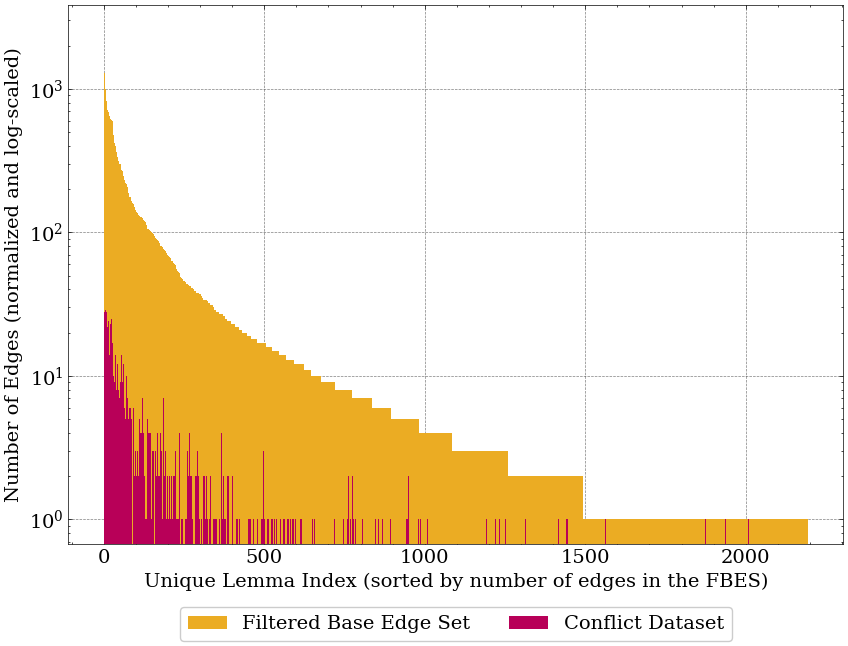
\includegraphics[width=0.8\textwidth]
{dataset_lemma_distribution/lemma_distribution_dataset_conflicts_1-2_pred_wildcard_full_dataset_conflicts_1-2_pred_wildcard_subsample-2000.png}
\caption{Distribution of unique lemmas in the \gls{fbes} and \gls{cd}}
\label{fig:dataset-lemma-distribution}
\end{figure}


\begin{algorithm}
\begin{enumerate}
	\item Create a list of tuples \(t\) of edges and their corresponding predicate lemma: \\ \(L = [(l_k, e_i), ...]\) with \(k \in \{0,...,m\}\) and \(i \in \{0,...,n\}\)
	\item Sort this list by the number of tuples containing a predicate lemma to create the list: \\ \(L_{sort} = [(l_0, e_0), ... (l_m, e_n)]\), so that:
	\begin{itemize}
		\item \(n_k\) is the number of tuples containing a lemma \(l_k\)
		\item \(t_j\) with \(j > i\) is a tuple wich sorted after tuple \(t_i\)
		\item \(n_o >= n_p\) if \(t_i = (l_o, e_i)\) and \(t_j = (l_p, e_j)\)
	\end{itemize}			
	\item Split the list \(L_{sort}\) into \(n_{b}\) bins.
	\item Uniformly sample \(n_{sb}\) tuples from each bin.
	\item Build a set of all edges \(e\) contained in the sampled tuples.
\end{enumerate}
\caption{Dataset sampling algorithm}
\label{algo:dataset-sampling}
\end{algorithm}

The subsampled dataset size resulting from this sampling method is \(n_{s} = n_{b} * n_{sb}\). Given \(n_{s} = 2000\), the values \(n_b = 10\) and \(n_{sb} = 200\) were chosen for sampling the \gls{cd}.


\subsubsection{Labelling}
The labelling task is shared between the three annotators. A given edge will be either labeled as \textit{conflict} or \textit{no conflict} by an annotator following the definition given in \cref{sec:conflict-definition}. Because of the aforementioned time constraints, every edge is only labeled by one annotator. To nonetheless ensure a consistent labelling among all annotators, a set of 50 edge is labelled by all three annotators. Every edge for which a disagreement in labelling occurs between at least two of the annotators, is inspected to reach an agreement on the label. Utilizing this process, the annotators understanding of what constitutes an expression of conflict is refined. Following this preliminary step, the \(n_s\) edges of the dataset are equally distributed among the three annotators and individually labelled by them.

% It was confirmed that the percentage of edges that represent an expression of conflict in relation to all edges in the subset given to an annotator did not vary more than ... among all three annotators.

\subsection{Edge Set Comparison}
The \gls{cd} is the result of the filtering, sampling and labelling described above. The size of the Worldnews-\gls{sh}, \gls{bes}, \gls{fbes} and \gls{cd} are listed in \cref{tab:dataset-descriptions} for comparison. If applicable, the number of unique lemmas as well as the number and percentage of edges which are labelled as an expression of conflict and of those which are not are also noted. \Cref{tab:example-edges} in \cref{app-sec:example-edges} list the content of randomly sampled exemplary edges for the Worldnews-SH, the \gls{fbes} and the \gls{cd}. For the latter, the corresponding edge labels are also listed.


\begin{table}
\centering
\begin{tabular}{lrrrr}
\toprule
\multicolumn{1}{l}{Edge set name}	& \multicolumn{1}{c}{Number of} & \multicolumn{1}{c}{Number of}		& \multicolumn{1}{c}{Number of} 		& \multicolumn{1}{c}{Number of} \\
\multicolumn{1}{l}{} 				& \multicolumn{1}{c}{all edges} & \multicolumn{1}{c}{un. lemmas}			& \multicolumn{1}{c}{conflict edges} 	& \multicolumn{1}{c}{no conflict edges} \\
\multicolumn{1}{l}{} 				& \multicolumn{1}{c}{} 			& \multicolumn{1}{c}{}				& \multicolumn{1}{c}{(\% of all edges)} & \multicolumn{1}{c}{(\% of all edges)} \\
\midrule
Worldnews-\gls{sh}						& 479384		& -			& -					& - \\
Base Edge Set (\gls{bes})					& 71804		& -			& -					& - \\
Filtered \gls{bes} (\gls{fbes})					& 69380 		& 2195 		& - 					& - \\
Conflict Dataset (\gls{cd})				& 2000 		& 539 		& 599 (29.95 \%) 	& 1401 (70.05 \%) \\
\bottomrule
\end{tabular}
\caption{Number of edges, number of unique lemmas and proportion of labels for the different edge sets}
\label{tab:dataset-descriptions}
\end{table}


\section{Evaluation Process}
In this evaluation multiple \textit{evaluation runs} are conducted. Each evaluation run correspond to a \gls{shpm} process in which a pattern is matched against the \gls{cd}. In the case of patterns utilizing \gls{ness} this requires that additional parameters in form of an \textit{\gls{ness} configuration} are given to the matching process. An evaluation run is described by an \textit{evaluation (run) configuration}. For each evaluation run the \textit{evaluation metrics} are computed. 

\subsection{Evaluation Run Configurations}
An evaluation configuration consists of the following parameters:
\begin{itemize}
	\item Conflict Pattern
	\item \gls{ness} Configuration (in case of \gls{ness-shpm}): 
	\begin{itemize}
		\item \gls{ness} model
		\item Similarity Threshold 
		\item Use  all tokens (in the case of \gls{cness}) 
		\item Reference Edge Set (in the case of \gls{cness}) 
	\end{itemize}
\end{itemize}


\paragraph{Conflict Patterns}
The four conflict patterns used in this evaluation are described in detail in \cref{sec:sh-patterns}. An overview of the properties of these patterns can be seen in \cref{tab:evaluation-patterns}.


\paragraph{NESS models}
The neural embedding model -- or \gls{ness} model -- may be one of those described in \cref{sec:fixed-word-embedding-matcher} and \cref{sec:contextual-embedding-matcher}: \textit{word2vec}, \textit{conceptnetnumber-batch}, \textit{E5} and \textit{GTE}. In case of a \gls{fness} utilizing conflict pattern, the \gls{ness} model name is added in its shortened form: word2vec as \textit{w2v} and conceptnet-numberbatch as \textit{cn}


\paragraph{Similarity Thresholds}
In this evaluation the similarity threshold \(t_s\) is always selected from a range of thresholds \(r_t = \{0, 0.01, ...,  0.99, 1.00\}\), i.e. \(t_s \in r_t\). This results in 101 different values of \(t_s\).


\paragraph{Reference Edge Sets}
Multiple \gls{res}  are randomly sampled from the set of edges in the \gls{cd}, which are labelled as "conflict". These edges are then excluded from the dataset, to avoid introducing data from the test dataset to the system that is being evaluated. To compare the effect of different sample sizes, differently sized sets are drawn. To compare the effect of different samples, different samples are drawn. A \gls{res} with ID \textit{N-X} has \(N \in \{1, 3, 10\}\) samples and is from sample draw \(X \in \{1, 2, 3, 4, 5\}\). This results in 15 different \gls{res}s in total. The specific sets that have been sampled can be seen in \cref{app-sec:ref-edge-sets}.


\subsubsection{Evaluation Run Names}
\label{sec:eval-run-names}
An evaluation run name has the form: \texttt{CP NM-AT r-N-X t-TS}

%\begin{center}
%\texttt{<CP> <NM>-<AT> <r-N-X> <t-TS>}
%\end{center}
In a specific evaluation run name, the placeholders (capitalised letters) are replaced with actual values. Such a name always begins with the conflict pattern (CP) name in its shortened form: \textit{original}, \textit{semsim-fix}, \textit{semsim-fix-lemma} or \textit{semsim-ctx}. This is followed by the \gls{ness} model (NM) name. If the \gls{ness} type is \gls{cness}, the usage of the all-tokens (AT) option is indicated by adding \texttt{-at} to the model name. Also in case of \gls{cness}, the reference edge set ID N-X is indicated by appending \texttt{r-N-X}. For all \gls{ness} utilizing evaluation runs, the similarity threshold \(t_s\) is indicated by appending \texttt{t-TS}, where \texttt{TS} is the value of \(t_s\).



\subsubsection{Specification of Evaluation Run Configurations}
\label{sec:evaluation-configurations}
The configurations for all evaluation runs that are conducted in this case study are specified in \cref{tab:evaluation-run-configs}. All possible parameter combinations of an evaluation configuration, i.e. the conflict pattern and the \gls{ness} parameters, are evaluated. The total number of conducted evaluation runs therefore amounts to 6465.\footnote{1 (original) + 2 (semsim-fix and semxim-fix-lemma) * 2 (\gls{fness} models) * 101 (\gls{st}s) \\ + 1 (semsim-ctx) * 2 (\gls{cness} models) * 2 (all tokens) * 15 (ref. edge sets) * 101 (\gls{st}s)} In \cref{tab:evaluation-run-configs} the different values for the reference edge set ID and the \gls{st} are omitted. The \textit{random} evaluation run configuration relates to a hypothetical evaluation run in which edges are uniformly randomly matched. 


\subsection{Evaluation Metrics}
\label{sec:evaluation-metrics}
Using the information provided by the dataset labels it is determined whether a match is correct or not. If an edge is matches in a given evaluation run and is labeled as "conflict" in the dataset, it is considered a \textit{true positive} (TP). If an edge matches but is labeled "no conflict", it is considered a \textit{false positive} (FP). The \textit{true negatives} (TN) and \textit{false negatives} (FN) are determined analogously  by examining the non-matching edges. Based on the TP, FP, TN and FN the metrics \textit{precision}, \textit{recall} and \textit{F1-score} are computed.

Jointly inspecting precision and recall of a system allows to asses its \textit{retrieval performance}, since there generally exists a trade-off between these system properties. The F1-Score is an established metric, which integrates precision and recall and therefore acts as an measurement of overall retrieval performance in this evaluation.

\paragraph{Relationship of Similarity Threshold and Recall}
It can be generally stated that the recall (\(r\)) of \gls{ness-shpm} in relation to the similarity threshold (\(r(t_s)\)) is strictly monotonically decreasing, since the set of points in embedding space that is inside of the similarity boundary consistently gets smaller with increasing threshold.


\begin{table}
\centering
\begin{tabular}{lcccc}
\toprule
\multicolumn{1}{l}{Pattern name}		& \multicolumn{1}{c}{Lemma}		& \multicolumn{1}{c}{\gls{ness}}	& \multicolumn{1}{c}{Includes}		& \multicolumn{1}{c}{Requires} \\
\multicolumn{1}{l}{} 				& \multicolumn{1}{c}{based} 		& \multicolumn{1}{c}{type} 		& \multicolumn{1}{c}{ref. words} 	& \multicolumn{1}{c}{ref. edges} \\
\midrule
Original conflict pattern (\ref{pat:original-conflict})					& Yes 		& - 		& -			& - \\
semsim-fix conflict pattern (\ref{pat:semsim-fix-conflict})				& No		& Fixed		& Yes		& No \\
semsim-fix-lemma conflict (\ref{pat:semsim-fix-lemma-conflict}) 		& Yes 		& Fixed		& Yes		& No \\
semsim-ctx conflict patter (\ref{pat:semsim-ctx-conflict})				& No		& Contextual	& No		& Yes \\
\bottomrule
\end{tabular}
\caption{Properties of the conflict patterns used in the evaluation}
\label{tab:evaluation-patterns}
\end{table}


\begin{table}
\centering
\begin{tabular}{llcc}
\toprule
\multicolumn{1}{l}{Evaluation Run Name} & \multicolumn{1}{l}{Conflict Pattern} & \multicolumn{2}{c}{\gls{ness} Configuration} \\
\cmidrule{3-4}
\multicolumn{1}{l}{}   & \multicolumn{1}{l}{}  & \multicolumn{1}{c}{\gls{ness} Model}	& \multicolumn{1}{c}{all tokens} \\
\midrule
original                       & original                     & -                          & -                \\
semsim-fix w2v                 & semsim-fix                   & word2vec                   & -                \\
semsim-fix cn                 & semsim-fix                   & conceptnet-numbatch                      & -      \\
semsim-fix-lemma w2v           & semsim-fix-lemma             & word2vec                   & -                \\
semsim-fix-lemma cn           & semsim-fix-lemma             & conceptnet-numbatch                      & -      \\
semsim-ctx e5 r-N-X                & semsim-ctx                   & E5                         & No           \\
semsim-ctx gte r-N-X              & semsim-ctx                   & GTE                        & No            \\
semsim-ctx e5-at r-N-X             & semsim-ctx                   & E5                         & Yes          \\
semsim-ctx gte-at r-N-X           & semsim-ctx                   & GTE                        & Yes           \\
\end{tabular}
\caption{Evaluation Run Configurations}
\label{tab:evaluation-run-configs}
\end{table}


\section{Evaluation Results}
\label{sec:evaluation-results}
In this section the results of the evaluation runs which are defined by the evaluation configurations in \cref{sec:evaluation-configurations} are examined. Different perspectives on the result data are constructed in the form of tables and plots to enable answering the research questions. The following subsections each represent one perspective and conclude with significant observations that can be made based on it.

\subsubsection{Result Data Description Concepts}
To facilitate constructing insightful perspectives on the result data, some novel concepts for its description are introduced in the following.

\paragraph{Evaluation Run Sets}
Multiple evaluation runs can be grouped into an \gls{ers} according to their shared configuration parameter values. The naming convention for an \gls{ers} follows the evaluation run naming convention described in \cref{sec:eval-run-names}. The parameters values that are not shared among the evaluation runs in the \gls{ers} are omitted from the name or replaced by the wildcard symbol \texttt{*}. The placeholders (capitalised letters) are used to refer to an E\gls{sr} of a generic form with fixed parameter values without specifying these values.  By surrounding a part of the \gls{ers} name with parentheses \texttt{(*)}, it is indicated that this part is omitted if unsuitable. 

Examples are given to illustrate this:
\begin{itemize}
	\item An \gls{ers} of all evaluation runs utilizing any form of \gls{ness} with \(t_s = 0.5\) is named: \\ \texttt{semsim-* t-0.5}
	\item An \gls{ers} of all evaluation runs utilizing \gls{fness} with an unspecified but fixed \gls{ness} model has the form: \\ \texttt{semsim-fix(-*) NM} 
	\item An \gls{ers} of all evaluation runs utilizing \gls{ness} with all parameters (that are applicable) fixed but unspecified, except for the specific value \(t_s = 0.5\), has the form: \\ \texttt{semsim-* NM(-AT) (r-N-X) t-0.5}
\end{itemize}

\paragraph{Best F1-Score Evaluation run} The \textit{best F1-Score evaluation run} refers to the evaluation run with the highest F1-Score in an \gls{ers} corresponding to a \gls{ness} utilizing evaluation configuration where every parameter except for \(t_s\) is fixed. Such an \gls{ers} is generally named \texttt{semsim-* NM(-AT) (r-N-X)}. The corresponding F1-score is also simply referred to as \textit{best F1-score}.
%This means among the results for all similarity threshold in the given threshold range for a given evaluation run, the \gls{st} that results in the highest F1-score is selected. The scores of the other evaluation metrics also correspond to this \gls{st}.

\paragraph{Mean Reference Edge Set Evaluation Runs}
A \textit{mean reference edge set evaluation run} is constructed from the mean value of all evaluation scores for the evaluation runs in an \gls{ers} of the form \texttt{semsim-ctx NM-AT r-N-* t-TS}. This means for every \(t_s\) the mean of the corresponding evaluation scores of all reference edge sets of the same size is computed. In the following these synthetical evaluation runs are referred to in this form: \texttt{semsim-ctx NM-AT r-N-mean}
%These mean evaluation runs are primarily relevant for visualisation in the result plots (see \cref{sec:eval-metrics-vs-st}).

\paragraph{Mean Reference Edge Set Best F1-Score Evaluation Metric Scores}
The \textit{mean reference edge set (RES) best F1-Score evaluation metric scores} are the mean values of all evaluation scores corresponding to the best F1 score for all evaluation runs in an \gls{ers} of the form \texttt{semsim-ctx NM-AT r-N-*}. In the following these evaluation metric scores will be referred to in this form: \texttt{semsim-ctx NM-AT r-N-mean-best}
%For example \textit{semsim-ctx e5-at r-10-best-mean} refers to the mean of best F1 scores for all evaluation runs that use the semsim-ctx conflict pattern, the e5 model with all-tokens enabled and a reference edge set of size ten. 



\subsection{Best F1-Score based Evaluation Run Comparison}
\label{sec:best-f1-score-eval-run-comparison}
\Cref{tab:best-f1-score-mean-best} shows the evaluation scores for all evaluation metrics of the best F1-score evaluation runs for the original conflict pattern evaluation run and all evaluation runs utilizing \gls{fness}. For the evaluation runs utilizing \gls{cness} only the mean \gls{res} best F1-score evaluation metric scores and the standard deviation of the best F1-scores for the corresponding \gls{ers}s are shown. The \(t_s\) value listed for the mean \gls{res} best F1 score evaluation metrics is the mean of all \(t_s\) values for the best F1-scores in the corresponding \gls{ers}s.

In \cref{tab:best-f1-score-mean-best-semsim-ctx} and \cref{tab:best-f1-score-mean-best-semsim-ctx-at} of \cref{app-sec:result-tables} the best F1-score evaluation run results can be seen for evaluation runs utilizing \gls{cness} with all-tokens disabled and enabled respectively. These tables also list the hypothetical best F1-score evaluation for run the mean reference edge set evaluation runs. Additionally the mean standard deviation for these \gls{ers}s is shown, i.e. the mean of the standard deviations of the F1-score for every \gls{ers} of the form \texttt{semsim-ctx NM-AT r-N-* t-TS}.

\begin{table}[htp]
\centering
\begin{tabular}{lllrrrrrr}
\toprule
\multicolumn{4}{l}{Evaluation Run Name} & \multicolumn{1}{c}{Prec.} & \multicolumn{1}{c}{Rec.} & \multicolumn{2}{c}{(Best) F1-Score}\\
\cmidrule{1-4}\cmidrule{7-8}
\multicolumn{1}{l}{CP} & \multicolumn{1}{l}{NM} & \multicolumn{1}{l}{RES} & \multicolumn{1}{c}{\(t_s\)} & \multicolumn{3}{l}{} & \multicolumn{1}{c}{Std. Dev.} \\
\midrule
random &  &  & - & 0.300 & 0.500 & \textbf{0.375} & - \\
\hline
original &  &  & - & 0.706 & 0.209 & \textbf{0.322} & - \\
\hline
semsim-fix & cn &  & 0.25 & 0.479 & 0.524 & 0.500 & - \\
semsim-fix & w2v &  & 0.27 & 0.483 & 0.533 & \textbf{0.507} & - \\
\hline
semsim-fix-l. & cn &  & 0.30 & 0.492 & 0.558 & \textbf{0.523} & - \\
semsim-fix-l. & w2v &  & 0.33 & 0.460 & 0.553 & 0.502 & - \\
\hline
semsim-ctx & e5 & r-1-mean-best & 0.65 & 0.392 & 0.772 & 0.518 & +/- 0.025 \\
semsim-ctx & gte & r-1-mean-best & 0.59 & 0.336 & 0.879 & 0.483 & +/- 0.025 \\
semsim-ctx & e5 & r-3-mean-best & 0.68 & 0.399 & 0.818 & 0.536 & +/- 0.021 \\
semsim-ctx & gte & r-3-mean-best & 0.65 & 0.365 & 0.799 & 0.499 & +/- 0.016 \\
semsim-ctx & e5 & r-10-mean-best & 0.72 & 0.416 & 0.790 & \textbf{0.544} & +/- 0.020 \\
semsim-ctx & gte & r-10-mean-best & 0.68 & 0.382 & 0.812 & 0.517 & +/- \textbf{0.010} \\

\hline
semsim-ctx & e5-at & r-1-mean-best & 0.69 & 0.369 & 0.841 & 0.509 & +/- 0.016 \\
semsim-ctx & gte-at & r-1-mean-best & 0.66 & 0.335 & 0.882 & 0.483 & +/- 0.021 \\
semsim-ctx & e5-at & r-3-mean-best & 0.72 & 0.378 & 0.821 & 0.516 & +/- 0.011 \\
semsim-ctx & gte-at & r-3-mean-best & 0.70 & 0.336 & 0.876 & 0.485 & +/- 0.017 \\
semsim-ctx & e5-at & r-10-mean-best & 0.74 & 0.382 & 0.843 & \textbf{0.525} & +/- 0.012 \\
semsim-ctx & gte-at & r-10-mean-best & 0.72 & 0.338 & 0.900 & 0.491 & +/- \textbf{0.008} \\
\bottomrule
\end{tabular}
\caption{Evaluation scores corresponding to best F1-scores for all evaluation runs}
\label{tab:best-f1-score-mean-best}
\end{table}

\subsubsection{Significant Observations}
\begin{enumerate}[label=\arabic{listcounter}.\arabic*]
\refstepcounter{listcounter}% Increment the list counter
%	\item The random evaluation run achieves a higher F1-score than the original conflict pattern evaluation run
	\item All evaluation runs utilizing \gls{ness} achieve a best F1-score that is higher than the F1-score of the random evaluation run and the original evaluation run \label{obs-itm:ness-higher-best-f1}
	\item \gls{cness} achieves achieves a higher F1-score than \gls{fness} by 4.0\%, when comparing the highest F1-scores achieved among all \gls{fness} utilizing evaluation runs and the highest mean \gls{res} best F1 score achieved among all \gls{cness} utilizing evaluation runs (\texttt{semsim-fix-lemma cn t-0.30} and \texttt{semxim-ctx e5 r-10-mean-best}) \label{obs-itm:cness-higher-best-f1-than-fness}
	\item Lemma based \gls{fness} achieves a higher F1-score than non-lemma \gls{fness} by 3.2\%, when comparing the highest F1-scores achieved by evaluation runs utilizing one of the two variants (\texttt{semsim-fix w2v t-0.27} and \texttt{semsim-fix-lemma cn t-0.30}) \label{obs-itm:lemma-based-fness-higher-best-f1}
	\item For lemma based \gls{fness}, the conceptnet-numberbatch model achieves a higher best F1-score than the word2vec model by 4.2\% \\ (\texttt{semsim-fix-lemma cn t-0.30} vs \texttt{semsim-fix-lemma w2v t-0.33}) \label{obs-itm:lemma-fness-cn-better-than-w2v}
	\item For not lemma based \gls{fness}, the word2vec model achieves a higher best F1-score than the conceptnet-numberbatch model by 1.4\% \\ (\texttt{semsim-fix w2v t-0.27} vs \texttt{semsim-fix cn t-0.25}) \label{obs-itm:word-fness-w2v-better-than-cn}
	\item \gls{cness} with the \gls{at} option disabled achieves a higher or equal mean \gls{res} best F1-score than \gls{cness} with \gls{at} option enabled in 6/6 (100\%) direct comparisons \\(\texttt{semsim-ctx NM r-N-mean-best} vs \texttt{semsim-ctx NM-at r-N-mean-best}) \label{obs-itm:cness-better-without-AT}
	\item \gls{cness} with the E5 model achieves a higher or equal mean \gls{res} best F1-score than \gls{cness} with the GTE model in 6/6 (100\%) direct comparisons \\ (\texttt{semsim-ctx e5-* r-N-mean-best} vs \texttt{semsim-ctx gte-* r-N-mean-best}) \label{obs-itm:cness-e5-better-than-gte}
	\item \gls{cness} with the \gls{at} option enabled has a lower standard deviation of best F1-score than \gls{cness} with the \gls{at} option disabled in 5/6 (83\%) direct comparisons \\ (\texttt{semsim-ctx NM-at r-N-mean-best} vs \texttt{semsim-ctx NM r-N-mean-best}) \label{obs-itm:cness-lower-variation-with-at}
%	\item \gls{cness} with the gte model has a lower standard deviation of best F1-score than \gls{cness} with the e5 model in 4/6 (67\%) direct comparisons \\ (\texttt{semsim-ctx gte-* r-N-mean-best} vs \texttt{semsim-ctx e-* r-N-mean-best})
%	\item For \gls{cness} with the \gls{at} option disabled, the gte model has a lower standard deviation of best F1-score than the e5 model in 3/3 (100\%) direct comparisons \\ (\texttt{semsim-ctx gte r-N-mean-best} vs \texttt{semsim-ctx e5 r-N-mean-best})
\end{enumerate}


\subsection{Evaluation Metric vs. Similarity Threshold}
\label{sec:eval-metrics-vs-st}

These plots visualise the resulting evaluation scores for the different evaluation metrics in relation to different values for the similarity threshold. 

\Cref{fig:best-f1-per-pattern} shows the F1-score vs. the \gls{st} for the best performing evaluation runs for each conflict pattern. That means for every conflict pattern, this shows the evaluation run(s) with the configuration that resulted in the highest best F1-score. For the \texttt{random} and \texttt{original} evaluation runs, there is obviously no configuration to choose from. 

For the \gls{fness} utilizing evaluation runs, the evaluation run with the highest F1-score in the \gls{ers}s of the form \texttt{semsim-fix(-lemma) NM} is selected. This means for the semsim-fix and semxim-fix-lemma conflict patterns the corresponding best F1-score evaluation runs of the best performing model are selected..

For the \gls{cness} utilizing evaluation runs, the evaluation runs which correspond to highest mean \gls{res} best F1-score are selected. This means the \gls{ers} of the form \texttt{semsim-ctx NM-AT r-N-*} which resulted in the highest mean value of best F1-scores. This \gls{ers} consists of five evaluation runs, wich each have the form \texttt{semsim-ctx NM-AT r-N-X}. The F1-scores for these runs are plotted with a lighter curve. The additional synthetical \texttt{semsim-ctx NM-AT r-N-mean} score is plotted with a normally bold curve. 

% All evaluation runs  evaluation runs correspond to those highlighted by bold letters in \cref{tab:best-f1-score-mean-best}.

\Cref{fig:prec-rec-best-semsim} follows the same concept as \cref{fig:best-f1-per-pattern}, but instead of the F1-score this plot shows the scores of precision and recall vs. the \gls{st}. Also in the selection of evaluation runs, the semsim-fix (not lemma) conflict pattern based evaluation runs are excluded.

The plots in this section are selected because they are deemed to be most relevant for the following. A more comprehensive comparison of the different evaluation runs from this perspective can be found in \cref{app-sec:eval-metric-vs-st-plots}.

%This result in lines parallel to the x-axis for the original conflict pattern, since it does not depend on a \gls{st}. It can therefore be seen as a baseline.

\paragraph{Active Similarity Threshold Range}
To facilitate the description of observation for this perspective on the result data, the concept of the \textit{active similarity threshold range} (ASTR) is introduced. For a given E\gls{sr} of the form \texttt{semsim-* NM(-AT) (r-N-X)}, the ASTR describes the range of \(t_s\) for which the recall (\(r\)) that is achieved by these evaluation runs is \(r \neq r_{max} = 1 \) and \(r \neq r_{min}\). Here \(r_{min}\) and \(r_{max}\) are the lowest and highest recall values, which correspond to \(t_{s1}\) <= \(t_{s2}\), since the function \(r(t_s)\) is monotonically decreasing.

\begin{figure}[htp]
 \centering
 \begin{subfigure}{\textwidth}
	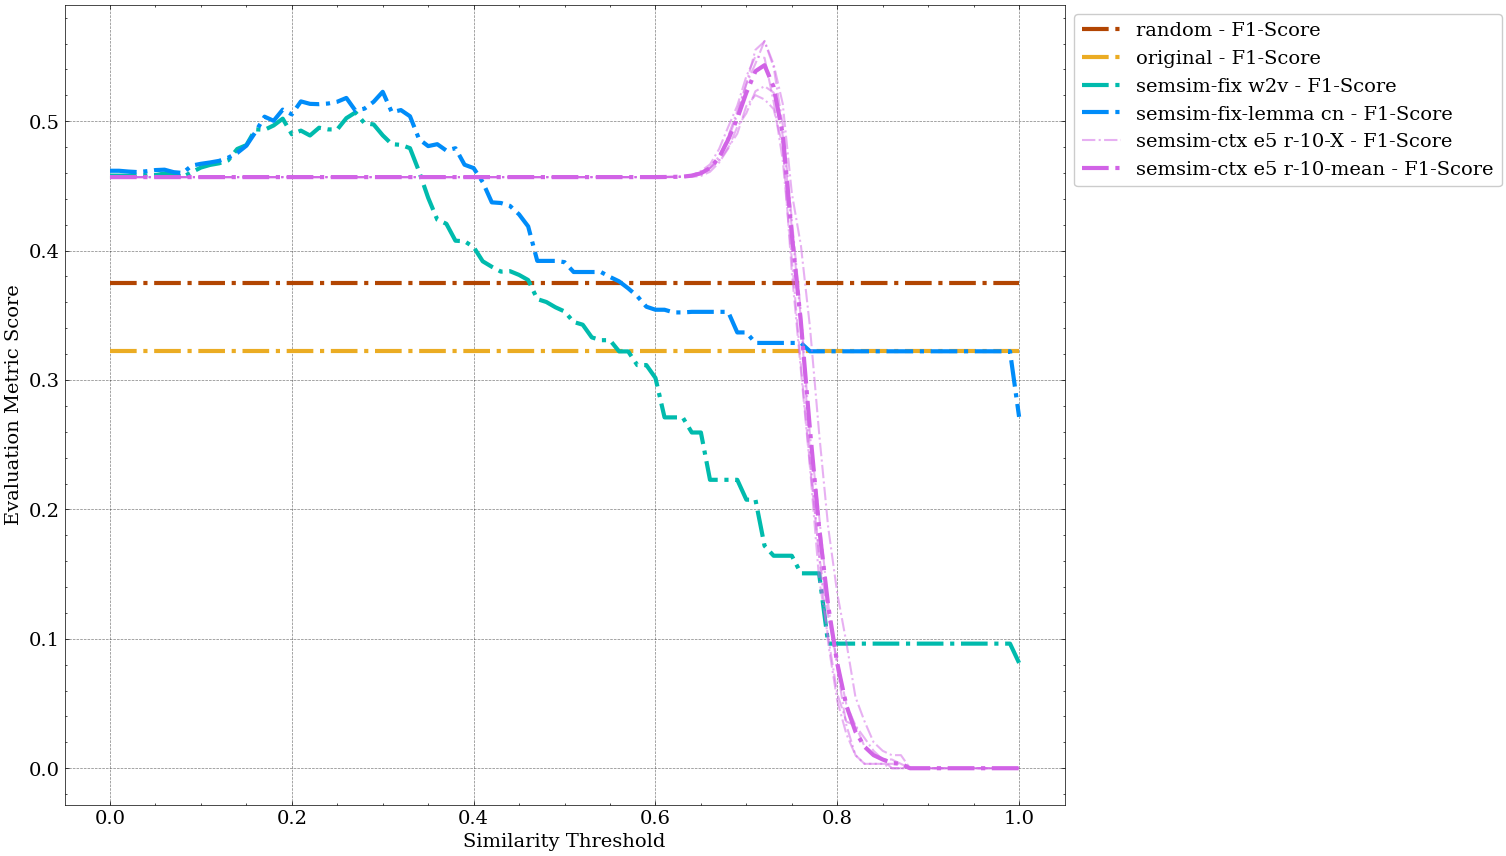
\includegraphics[width=\textwidth]{dataset_conflicts_1-2_pred_wildcard_subsample-2000_evaluation_original_vs_semsim-fix_w2v_vs_semsim-fix-lemma_cn_vs_semsim-ctx_nref-10_e5_f1}
	\caption{F1-score vs. \gls{st} for the evaluation runs \texttt{random}, \texttt{original}, \texttt{semsim-fix w2v}, \texttt{semsim-fix-lemma cn} and \texttt{semsim-ctx e5 r-10-X}}
	\label{fig:best-f1-per-pattern}
 \end{subfigure}
 \newline
 \newline
 \begin{subfigure}{\textwidth}
	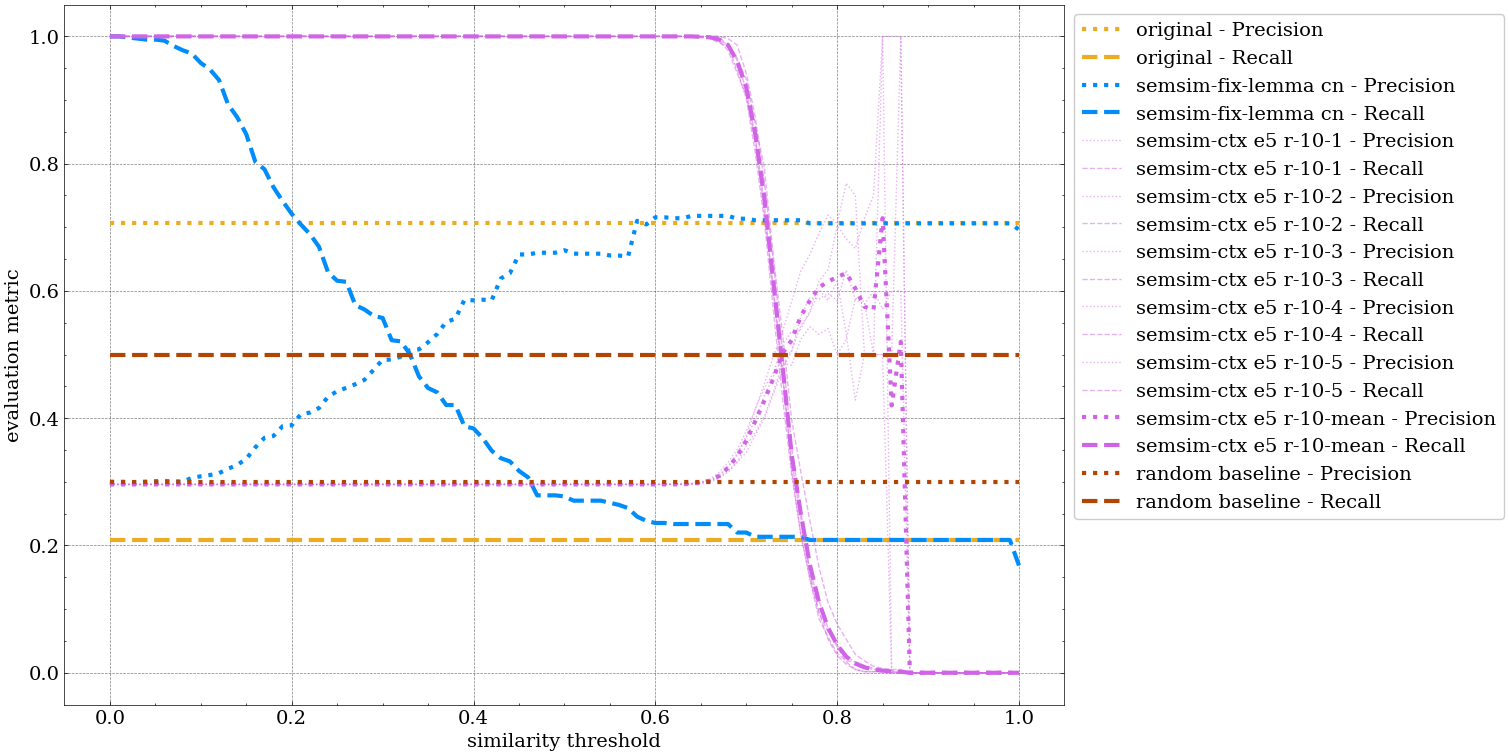
\includegraphics[width=\textwidth]{dataset_conflicts_1-2_pred_wildcard_subsample-2000_evaluation_original_vs_semsim-fix-lemma_cn_vs_semsim-ctx_nref-10_e5_precision-recall}
	\caption{Precision and  recall vs. \gls{st} for the evaluation runs \texttt{random}, \texttt{original}, \texttt{semsim-fix-lemma cn} and \texttt{semsim-ctx e5 r-10-X}}
	\label{fig:prec-rec-best-semsim}
 \end{subfigure}
 \caption{Evaluation metric scores vs. similarity threshold values}
\end{figure}

\subsubsection{Significant Observations}
\begin{enumerate}[label=\arabic{listcounter}.\arabic*]
\refstepcounter{listcounter}% Increment the list counter
%	\item The best F1-score of the synthetic evaluation runs \texttt{semsim-ctx e5 r-10-mean} is higher than the highest F1 score in achieved by any of the evaluation runs in \texttt{semsim-fix-*}.
	\item The ASTR of \texttt{semsim-fix-lemma cn} is larger (\(0.0 < t_s < 1.0\)) than the ASTR of \texttt{semsim-ctx e5} (ca. \(0.625 < t_s < 0.875\)) \label{obs-itm:astr-lemma-fness-cn-higher-than-cness-e5}
	\item Generally the ASTR of \gls{ers}s of the form \texttt{semsim-fix-* NM} is larger than the the ASTR of \gls{ers}s of the form \texttt{semsim-ctx} (confer also \cref{fig:prec-rec-f1-semsim-fix-lemma}, \cref{fig:prec-rec-f1-semsim-fix-lemma-model} \cref{fig:prec-rec-f1-semsim-ctx-model} and \cref{fig:prec-rec-f1-semsim-ctx-at}) \label{obs-itm:astr-fness-higher-than-cness}
	\item The ASTRs are nearly equal for \gls{ers}s of the form \texttt{semsim-fix-* NM} \label{obs-itm:ASTR-equal-fness} (confer \cref{fig:prec-rec-f1-semsim-fix-lemma} and \cref{fig:prec-rec-f1-semsim-fix-lemma-model}) \label{obs-itm:astr-fness-equal}
	\item The ASTR of \gls{ers}s of the form \texttt{semsim-ctx gte-AT} begin at a lower value than for \gls{ers}s of the form \texttt{semsim-ctx e5-AT} (confer \cref{fig:prec-rec-f1-semsim-ctx-model} and \cref{fig:f1-semsim-ctx-model-at}) \label{obs-itm:astr-cness-gte-starts-earlier}
	\item The ASTR of \gls{ers}s of the form \texttt{semsim-ctx NM} begin at a lower value than for \gls{ers}s of the form \texttt{semsim-ctx NM-at} (confer \cref{fig:prec-rec-f1-semsim-ctx-at} and \cref{fig:f1-semsim-ctx-model-at}) \label{obs-itm:astr-cness-at-starts-earlier}
	\item The ASTRs end at nearly the same value for \gls{ers}s of the form \texttt{semsim-ctx NM-AT} \label{obs-itm:ASTR-equal-fness} (confer \cref{fig:prec-rec-f1-semsim-ctx-model}, \cref{fig:prec-rec-f1-semsim-ctx-at} and \cref{fig:f1-semsim-ctx-model-at}) \label{obs-itm:astr-cness-end-equal}

	\item The evaluation runs in the \gls{ers} \texttt{semsim-fix-lemma cn} achieve a higher F1 value than the evaluation run in the \gls{ers} \texttt{semsim-fix w2v} for nearly all values of \(t_s\) \label{obs-itm:lemma-fness-higher-f1-nearly-always}

	\item The precision of the evaluation run which achieves the highest precision among those in the synthetic E\gls{sr} \texttt{semsim-ctx e5 r-10-mean} (\(p_\text{max}\)) and the precision of the original evaluation run (\(p_\text{og}\)) are nearly equal (\(p_\text{max} \approx p_\text{og}\)) \label{obs-itm:cness-highest-precision-equal-original} 	
	\item The precision of evaluation run \texttt{semsim-fix-lemma cn}  correlates with the \gls{st} until it reaches the value achieved by the \texttt{original} evaluation run, where it plateaus \label{obs-itm:fness-st-precision-correlates}
	\item The precision of the evaluation runs in \gls{ers} \texttt{semsim-ctx e5} correlate with the \gls{st} until precision (\(p\)) and recall (\(r\)) reach approximately the same value (\(p \approx r \approx 0.5\)), after which it fluctuates (the specific fluctuation varies with the specific \gls{res}) \label{obs-itm:cness-st-precision-correlates-until-crosspoint}

	\item The precision achieved by evaluation runs in \gls{ers}s of the form \texttt{semsim-ctx e5 r-10-* t-TS} has a higher variation for \(t_s \geq 0.75\) than for \(t_s < 0.75\) \label{obs-itm:cness-precision-variation-higher-ASTR}
	\item The precision of the evaluation run which achieves the highest precision among those in the synthetic E\gls{sr} \texttt{semsim-ctx e5 r-10-mean} (\(p_\text{max}\)) and the precision of the original evaluation run (\(p_\text{og}\)) are nearly equal (\(p_\text{max} \approx p_\text{og}\)) \label{obs-itm:cness-highest-precision-equal-original} 	
	\item The evaluation metric scores of \texttt{semsim-fix-lemma cn t-1.00} are lower than those of the \texttt{original} evaluation run \label{obs-itm:fness-st-limit}

%	\item Precision (\(p\)) and recall (\(r\)) have the same value (\(p \approx r \approx 0.5\)) at specific similarity thresholds \(t_1\) and \(t_2\) for the two \gls{ers}s \texttt{semsim-fix-lemma cn} and \texttt{semsim-ctx e5}

\end{enumerate} 

 
%\begin{figure}[hp]
%\centering
%\includegraphics[width=\textwidth]
%%\includegraphics[width=0.85\paperwidth, center]
%{dataset_conflicts_1-2_pred_wildcard_subsample-2000_evaluation_original_vs_semsim-fix_w2v_vs_semsim-fix-lemma_cn_vs_semsim-ctx_nref-10_e5_f1}
%\caption{F1-score vs. \gls{st} for the best performing evaluation run configuration for each conflict pattern (including the original pattern)}
%\label{fig:best-f1-per-pattern}
%\end{figure}
%
%\begin{figure}[hp]
%\centering
%%\includegraphics[width=\textwidth]
%\includegraphics[width=\textwidth]
%{dataset_conflicts_1-2_pred_wildcard_subsample-2000_evaluation_original_vs_semsim-fix-lemma_cn_vs_semsim-ctx_nref-10_e5_precision-recall}
%\caption{Precision and  recall vs. \gls{st} for the evaluation runs \texttt{original}, \texttt{semsim-fix-lemma cn} and \texttt{semsim-ctx e5 r-10-X}}
%\label{fig:prec-rec-best-semsim}
%\end{figure}


%\begin{figure}
%\centering
%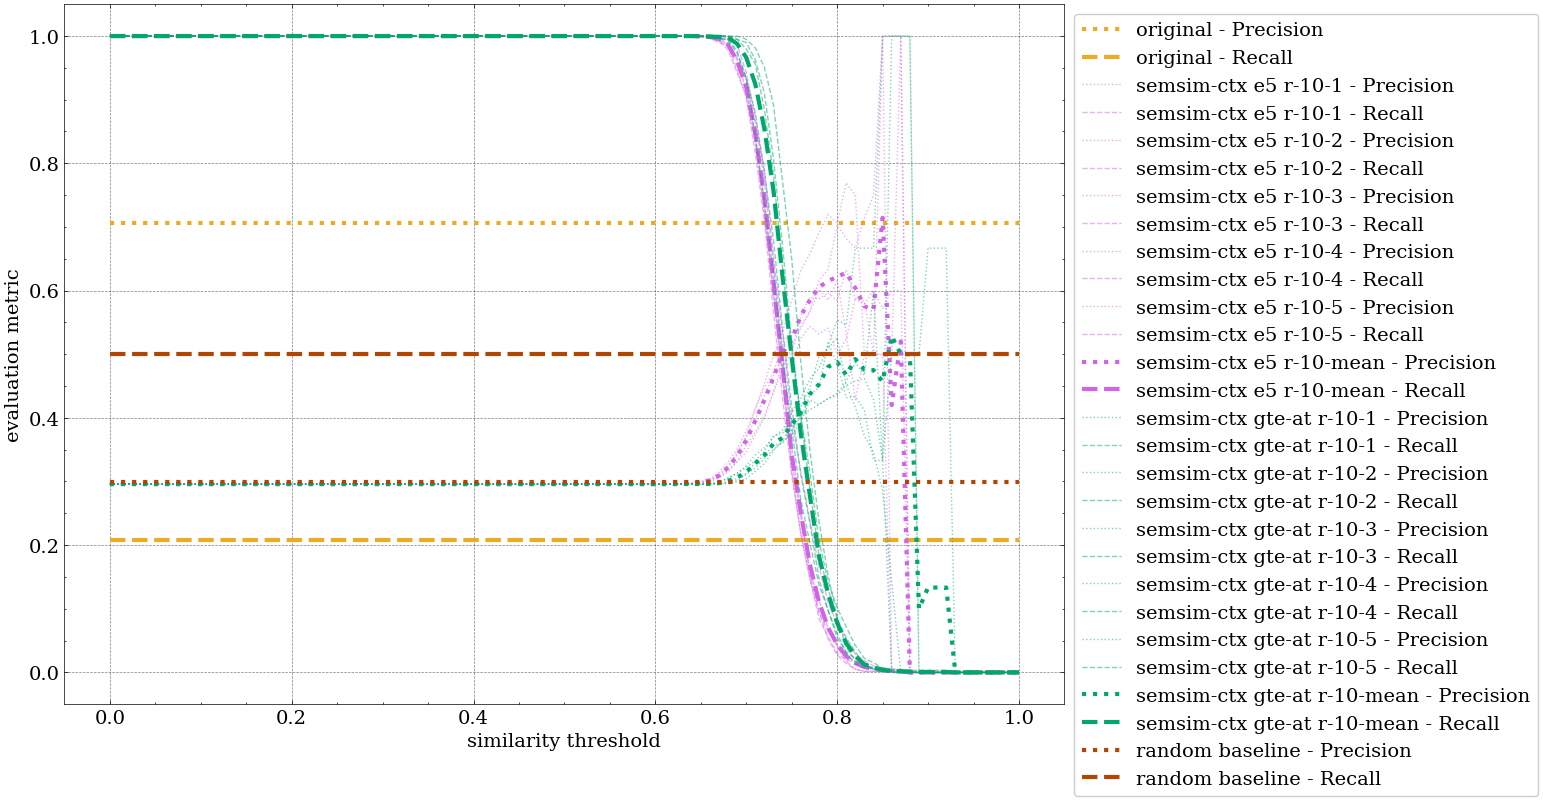
\includegraphics[width=\textwidth]{dataset_conflicts_1-2_pred_wildcard_subsample-2000_evaluation_original_vs_semsim-ctx_nref-10_e5_vs_gte-at_precision-recall}
%\caption{Caption for this figure}
%\label{fig:unique-label-2}
%\end{figure}


\subsection{Best F1-Score vs. Number of Reference Edges}
\label{sec:best-f1-vs-nref}
\Cref{fig:best-f1-vs-nref} visualises the relation of the number of reference edges and the best-F1 score. For this purpose the number of reference edges \texttt{N} is plotted versus the mean \gls{res} best F1-score for all \gls{ers}s of the form \texttt{semsim-ctx NM-AT r-N-*}.  The standard deviation of the best F1 scores for these \gls{ers}s is visualised by the shaded areas around the curves of the mean \gls{res} best F1-scores.

\begin{figure}
\centering
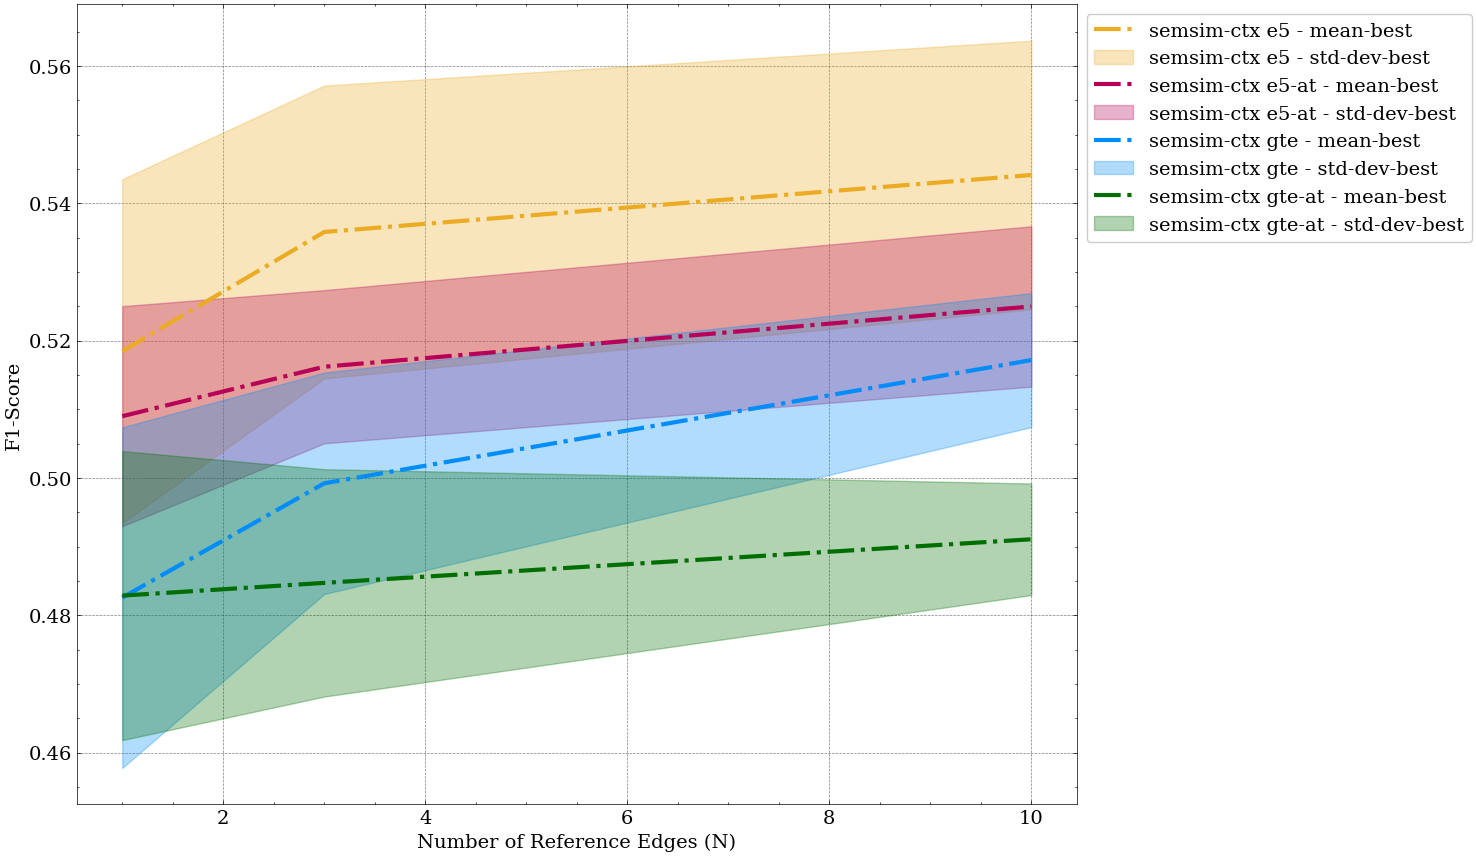
\includegraphics[width=\textwidth]
{/dataset_n_ref_edges/dataset_conflicts_1-2_pred_wildcard_subsample-2000_best-f1_nref_vs_f1}
\caption{Mean reference edge set best F1-score for the \gls{ers}s \texttt{semsim-ctx e5 r-N-*}, \texttt{semsim-ctx e5-at r-N-*}, \texttt{semsim-ctx gte-at r-N-*} and \texttt{semsim-ctx gte-at r-N-*}}
\label{fig:best-f1-vs-nref}
\end{figure}

\subsubsection{Significant Observations}
\begin{enumerate}[label=\arabic{listcounter}.\arabic*]
\refstepcounter{listcounter}% Increment the list counter
	\item The mean \gls{res} best F1-score of the evaluation runs in an \gls{ers} of the form \texttt{semsim-ctx NM(-AT) r-\(N_1\)-*} is higher than the mean \gls{res} best F1-score of the evaluation runs in an \gls{ers} of the form \texttt{semsim-ctx NM(-AT) r-\(N_2\)-*}, if \(N_2 > N_1\) for \(N_1, N_2 \in \{1, 3, 10\}\) \label{obs-itm:cness-more-refs-higher-mean-best-f1}
	\item The standard deviation of the mean \gls{res} best F1-score of the evaluation runs in an \gls{ers} of the form \texttt{semsim-ctx NM(-AT) r-\(N_1\)-*} is lower than the standard deviation of the mean \gls{res} best F1-score of the evaluation runs in an \gls{ers} of the form \texttt{semsim-ctx NM(-AT) r-\(N_2\)-*}, if \(N_2 > N_1\) for \(N_1, N_2 \in \{1, 3, 10\}\), except for \texttt{semsim-ctx et-at r-3-*} (\(sd_1 = 0.11\)) and \texttt{semsim-ctx et-at r-10-*} (\(sd_2 = 0.12\)) \label{obs-itm:cness-more-refs-lower-stddev-best-f1}
%	\item , where \(sd_2 > sd_2\)
\end{enumerate}



\subsection{Predicate Lemma based Evaluation Run Comparison}
In this section it is explored how the different \gls{ness} systems differ in which edges they match. This is done by following up on the concept of the predicate lemma introduced in \cref{sec:base-edge-set}. In \cref{sec:dataset-characteristics} one of the two desired characteristics of the dataset states that it should contain the largest possible number of edges per unique predicate lemma. Specifically it is of interest, how the \gls{cness} system performs in comparison to the \gls{fness} system for subsets of edges which share the same predicate lemma. Such a subset of edges of the conflict dataset is in the following referred to as \gls{ples}.


%\subsubsection{Evaluation Runs Representing the \gls{ness} System Types}
\paragraph{\gls{ness} Type Representatives}
Two evaluation runs are selected to represent the two versions of the \gls{ness} systems for the comparison. The lemma-based version of \gls{fness} is chosen here, because of its superior performance regarding best F1-score that is observed in \cref{sec:best-f1-score-eval-run-comparison} and \cref{sec:eval-metrics-vs-st}. Specifically, the evaluation runs \texttt{semsim-fix-lemma cn t-0.30} (evaluation run \textit{A}) and \texttt{semsim-ctx e5 r-10-2 t-0.72} (evaluation run \textit{B}) are selected as representatives of the \gls{fness} and \gls{cness} system respectively. These are the best performing evaluation runs regarding F1-score for the respective semsim conflict patterns (i.e. \gls{ness} system), which can be seen in \cref{tab:best-f1-score-mean-best} and \cref{tab:best-f1-score-mean-best-semsim-ctx}.\footnote{
The latter table specifically shows that the evaluation runs \texttt{semsim-ctx e5 r-1-2 t-0.67}, \texttt{semsim-ctx e5 r-10-2 t-0.72} and \texttt{semsim-ctx e5 r-10-4 t-0.72} all correspond to an F1 score \(s_\text{F1} = 0.56\). The evaluation runs utilizing the \gls{res}s of size \(N = 10\) are chosen over the one utilizing an \gls{res} of size \(N = 1\), because of their generally superior performance regarding F1 score, which is observed in \cref{sec:best-f1-vs-nref}. Among the two remaining evaluation runs, \texttt{semsim-ctx e5 r-10-2 t-0.72} is selected randomly.


%While the lemma-based \gls{fness} system is only able to match all or none of the edges in a \gls{ples}, the \gls{cness} system is potentially able to differentiate between "conflict" and "no conflict" given a \gls{ples}.
%It shall be noted there that the \gls{fness} system is able to differentiate between different verb forms forms corresponding to the same lemma, when using the semsim-fix and not the semsim-fix-lemma functional pattern. Nonetheless this is assumed to add relevant semantic differentiation capabilities to the \gls{fness} system based on the observed 

}

\subsubsection{PLES Evaluation Score based Evaluation Run Comparison}

\paragraph{Label Balance Ratio}
The \gls{lbr} measures how balanced the labels in a given set of labelled edges are. It is calculated by \cref{eq:label-balance-ratio}. Here \(n_\text{pos}\) and \(n_\text{neg}\) are the number of positively ("conflict") and negatively ("no conflict") labeled edges in the edge set.
An edge set with fully balanced labels has \(LBR = 1\) and completely unbalanced labeled edge set has \(LBR = 0\).

\begin{equation}
LBR = 1 - \left(\frac{\left|n_{\text{pos}} - n_{\text{neg}}\right|}{n_{\text{pos}} + n_{\text{neg}}}\right)
\label{eq:label-balance-ratio}
\end{equation}

The evaluation metrics are computed for evaluation run A and B for each \gls{ples}, along with metrics that measure distributional properties of a \gls{ples}. Namely the number of edges \(n_e\), the number of positively labeled and negatively labeled edges (\(n_\text{pos}\) and \(n_\text{neg}\)), the \gls{lbr}  and the entropy of a \gls{ples}.

\Cref{tab:predicate-lemma-highest-f1} lists the ten predicate lemmas for whose \gls{ples} the absolute difference in F1-score, which is achieved in the two evaluation runs, is the highest. Conversely \cref{tab:predicate-lemma-lowest-f1} lists the ten predicate lemma for whose \gls{ples} the difference in F1-score which is achieved in the tow evaluation runs is the lowest. In both tables the predicate lemmas have been filtered beforehand, so that only \gls{ples} with \(n_s >= 5\) samples are considered. Additionally the recalls (\(r_A, r_B\)) achieved by both evaluation runs regarding a \gls{ples} must fulfil the condition that \(r_A + r_B > 0\), i.e. at least the recall achieved by one of the evaluation runs must be non-zero. \Cref{tab:predicate-lemma-highest-f1-both-recall-non-zero} follows the same concept as \cref{tab:predicate-lemma-highest-f1}, except for the condition regarding the recalls being \(r_A * r_B > 0\), i.e. the recall achieved by the both evaluation runs must be non-zero. This second variant of the table is not shown for \cref{tab:predicate-lemma-lowest-f1}, because it only lists lemmas for whose \gls{ples} the F1-score achieved by both evaluation runs is zero.

Exemplary edges that correspond to the lemmas in \cref{tab:predicate-lemma-highest-f1} and \cref{tab:predicate-lemma-highest-f1-both-recall-non-zero} are shown in \cref{tab:example-edge-labels-eval-b-win} and  \cref{tab:example-edge-labels-eval-a-win}. They are presented in combination with the labels given in the dataset and those produced by both evaluation runs. Both tables contain two edges per lemma, with one edge labeled as "conflict" and the other as "no conflict". In \cref{tab:example-edge-labels-eval-b-win}, evaluation run B labels all edges correctly. Conversely, in \cref{tab:example-edge-labels-eval-a-win}, evaluation run B labels all edges incorrectly. Since evaluation run A can only produce the same label for every edge that corresponds to the same lemma, one edge per lemma is labeled correctly and one edge is labeled incorrectly by evaluation run A.

%An comparison of the actual labels that were produced  by evaluation runs A and B for all \gls{ples} corresponding to the lemmas in \cref{tab:predicate-lemma-highest-precision} can be found in \cref{app-sec:ples-eval-labels}.
%specifically in \cref{tab:ples-labels-1}, \cref{tab:ples-labels-2}, \cref{tab:ples-labels-3}, \cref{tab:ples-labels-4}, \cref{tab:ples-labels-5}, \cref{tab:ples-labels-6} and \cref{tab:ples-labels-7} 

%\Cref{tab:predicate-lemma-f1} lists the ten predicate lemmas for whose \gls{ples} the best F1-scores are achieved in both of the two evaluation runs.

%\begin{table}[hp]
%\centering
%\begin{tabular}{lrr|lrr}
%\toprule
%\multicolumn{3}{c|}{\texttt{semsim-fix-lemma cn} at \(t_s = 0.30\)} & \multicolumn{3}{c}{\texttt{semsim-ctx e5 r-10-2} at \(t_s = 0.72\)} \\ 
%\midrule
%Lemma      & F1-score & Num. of Samples & Lemma      & F1-score & Num. of Samples \\
%\midrule
%arrest     & 1.00     & 11            & arrest     & 1.00     & 11            \\
%accuse     & 0.97     & 33            & file       & 1.00     & 5             \\
%warn       & 0.93     & 24            & attack     & 1.00     & 12            \\
%slam       & 0.92     & 7             & accuse     & 0.95     & 33            \\
%attack     & 0.91     & 12            & slam       & 0.92     & 7             \\
%criticize  & 0.91     & 6             & criticize  & 0.91     & 6             \\
%detain     & 0.89     & 5             & shoot      & 0.89     & 5             \\
%shoot      & 0.89     & 5             & order      & 0.88     & 14            \\
%condemn    & 0.84     & 25            & detain     & 0.86     & 5             \\
%dismiss    & 0.80     & 6             & launch     & 0.86     & 14            \\ 
%\bottomrule
%\end{tabular}
%\caption{Top ten lemmas regarding F1-score with number of samples per lemma \(n_s >= 5\) \\
%for the evaluation runs \texttt{semsim-fix-lemma cn t-0.30} and \texttt{semsim-ctx e5 r-10-2 t-0.72}}
%\label{tab:predicate-lemma-f1}
%\end{table}
%

\begin{table}[p]
\centering
\begin{tabular}{lccccccc}
\toprule
Lemma      & F1 Diff. & F1 A & F1 B & \(n_e\) & \(n_\text{pos}\)/\(n_\text{neg}\) & \gls{lbr} & Entropy \\
\midrule
file       & 1.00      & 0.00           & 1.00           & 5               & 5/0     & 0.00 & 0.00 \\
order      & 0.88      & 0.00           & 0.88           & 14              & 7/7     & 1.00 & 1.00 \\
launch     & 0.86      & 0.00           & 0.86           & 14              & 8/6     & 0.86 & 0.99 \\
step       & 0.80      & 0.00           & 0.80           & 5               & 2/3     & 0.80 & 0.97 \\
target     & 0.77      & 0.00           & 0.77           & 8               & 6/2     & 0.50 & 0.81 \\
use        & 0.75      & 0.00           & 0.75           & 14              & 5/9     & 0.71 & 0.94 \\
block      & 0.73      & 0.00           & 0.73           & 8               & 4/4     & 1.00 & 1.00 \\
take       & 0.71      & 0.00           & 0.71           & 19              & 6/13    & 0.63 & 0.90 \\
open       & 0.67      & 0.00           & 0.67           & 8               & 1/7     & 0.25 & 0.54 \\
suspend    & 0.67      & 0.00           & 0.67           & 6               & 2/4     & 0.67 & 0.92 \\
build      & 0.67      & 0.00           & 0.67           & 6               & 1/5     & 0.33 & 0.65 \\
\cmidrule{7-8}
\multicolumn{6}{l}{} & \multicolumn{2}{c}{mean} \\
\multicolumn{6}{l}{} & 0.61 & 0.79 \\
\bottomrule
\end{tabular}
\caption{Top ten lemmas regarding the highest difference in F1-score between the evaluation runs with recalls \(r_A + r_B > 0\) and number of samples per lemma \(n_s >= 5\) for the evaluation runs \texttt{semsim-fix-lemma cn t-0.30} (A) and \texttt{semsim-ctx e5 r-10-2 t-0.72} (B)}
\label{tab:predicate-lemma-highest-f1}
\end{table}

\begin{table}[p]
\centering
\begin{tabular}{lccccccc}
\toprule
Lemma      & F1 Diff. & F1 A & F1 B & \(n_e\) & \(n_\text{pos}\)/\(n_\text{neg}\) & \gls{lbr} & Entropy \\
\midrule
accept     & 0.42      & 0.25           & 0.67           & 7               & 1/6     & 0.29 & 0.59 \\
strike     & 0.30      & 0.80           & 0.50           & 9               & 6/3     & 0.67 & 0.92 \\
capture    & 0.22      & 0.44           & 0.67           & 7               & 2/5     & 0.57 & 0.86 \\
seize      & 0.17      & 0.67           & 0.50           & 12              & 6/6     & 1.00 & 1.00 \\
deny       & 0.17      & 0.50           & 0.67           & 6               & 2/4     & 0.67 & 0.92 \\
suggest    & 0.17      & 0.33           & 0.50           & 5               & 1/4     & 0.40 & 0.72 \\
warn       & 0.12      & 0.93           & 0.81           & 24              & 21/3    & 0.25 & 0.54 \\
claim      & 0.12      & 0.43           & 0.55           & 22              & 6/16    & 0.55 & 0.85 \\
attack     & 0.09      & 0.91           & 1.00           & 12              & 10/2    & 0.33 & 0.65 \\
threaten   & 0.09      & 0.52           & 0.61           & 20              & 7/13    & 0.70 & 0.93 \\
approve    & 0.08      & 0.12           & 0.20           & 16              & 1/15    & 0.12 & 0.34 \\
\cmidrule{7-8}
\multicolumn{6}{l}{} & \multicolumn{2}{c}{mean} \\
\multicolumn{6}{l}{} & 0.50 & 0.76 \\
\bottomrule
\end{tabular}
\caption{Top ten lemmas regarding the highest difference in F1-score between the evaluation runs with recalls \(r_A \cdot r_B > 0\) and number of samples per lemma \(n_s >= 5\) for the evaluation runs \texttt{semsim-fix-lemma cn t-0.30} (A) and \texttt{semsim-ctx e5 r-10-2 t-0.72} (B). Demonstrating cases, where evaluation run B produces correct labels.}
\label{tab:predicate-lemma-highest-f1-both-recall-non-zero}
\end{table}


\begin{table}[htp]
\centering
\begin{tabular}{lccccccc}
\toprule
Lemma      & F1 Diff. & F1 A & F1 B & \(n_e\) & \(n_\text{pos}\)/\(n_\text{neg}\) & \gls{lbr} & Entropy \\
\midrule
arrest     & 0.00      & 1.00           & 1.00           & 11              & 11/0    & 0.00 & 0.00 \\
slam       & 0.00      & 0.92           & 0.92           & 7               & 6/1     & 0.29 & 0.59 \\
criticize  & 0.00      & 0.91           & 0.91           & 6               & 5/1     & 0.33 & 0.65 \\
shoot      & 0.00      & 0.89           & 0.89           & 5               & 4/1     & 0.40 & 0.72 \\
condemn    & 0.00      & 0.84           & 0.84           & 25              & 18/7    & 0.56 & 0.86 \\
dismiss    & 0.00      & 0.80           & 0.80           & 6               & 4/2     & 0.67 & 0.92 \\
tell       & 0.01      & 0.49           & 0.50           & 28              & 9/19    & 0.64 & 0.91 \\
accuse     & 0.02      & 0.97           & 0.95           & 33              & 31/2    & 0.12 & 0.33 \\
kill       & 0.02      & 0.66           & 0.64           & 77              & 38/39   & 0.99 & 1.00 \\
say        & 0.03      & 0.45           & 0.48           & 31              & 9/22    & 0.58 & 0.87 \\
\cmidrule{7-8}
\multicolumn{6}{l}{} & \multicolumn{2}{c}{mean} \\
\multicolumn{6}{l}{} & 0.46 & 0.68 \\
\bottomrule
\end{tabular}
\caption{Top ten lemmas regarding the lowest absolute difference in F1-score between the evaluation runs with recalls \(r_A + r_B > 0\) and number of samples per lemma \(n_s >= 5\) for the evaluation runs \texttt{semsim-fix-lemma cn t-0.30} (A) and \texttt{semsim-ctx e5 r-10-2 t-0.72} (B)}
\label{tab:predicate-lemma-lowest-f1}
\end{table}

\begin{table}[htp]
\centering
\begin{tabular}{l p{6cm} ccc}
\toprule
Lemma & Edge Content & Dataset & Eval. A & Eval. B \\
\midrule
%capture		& Video captures horror of Istanbul airport attack & no conflict & conflict & no conflict \\
% 			& Security Service of Ukraine Captured Russian Spy & conflict & conflict & conflict \\
%\hline
deny	& Turkish FM denies investigation claims on German firms & no conflict & conflict & no conflict \\
\cline{2-5}
		& Kenya to deny entry to Ebola states & conflict & conflict & conflict \\

\hline
claim	& Bangkok police claim reward in Erawan Shrine bomber hunt & no conflict & conflict & no conflict \\
\cline{2-5}
		& Isis claims responsibility for killing of Hindu priest in Bangladesh & conflict & conflict & conflict \\

\hline
%order 	& France orders Facebook to stop monitoring Facebook visitors who don't sign up & conflict & no conflict & conflict \\
%		& Putin orders combat readiness checks for troops in Russia's far east & no conflict & no conflict & no conflict  \\
%\hline
launch 	& ISIS launches assault on pro-Assad forces in western Syria & conflict & no conflict & conflict \\
\cline{2-5}
		& UK PM Cameron launches English language campaign for Muslim women & no conflict & no conflict & no conflict \\
\hline
step 	& Beijing Steps Up Crackdown on Hong Kong Lawmakers & conflict & no conflict & conflict \\
\cline{2-5}
		& Irish Prime Minister Enda Kenny to step down & no conflict & no conflict & no conflict \\
\bottomrule
\end{tabular}
\caption{Dataset labels and evaluation labels of exemplary edges for evaluation runs \texttt{semsim-fix-lemma cn t-0.30} (A) and \texttt{semsim-ctx e5 r-10-2 t-0.72} (B). Demonstrates cases, in which evaluation run B produces correct labels.}
\label{tab:example-edge-labels-eval-b-win}
\end{table}


\begin{table}[htp]
\centering
\begin{tabular}{l p{6cm} ccc}
\toprule
Lemma & Edge Content & Dataset & Eval. A & Eval. B \\
\midrule
take & Japanese porn industry takes first step toward recognizing it has a problem & no conflict & no conflict & conflict \\
\cline{2-5}
	 & How flash mob flamenco took on the banks & conflict & no conflict & no conflict \\
\hline
deny		& Indian government denies renewal of passport opposition lawyer over minor traffic rule violation & conflict & conflict & no conflict \\
\cline{2-5}
			& Russia denies ground troop in Syria & no conflict & conflict & conflict \\
\hline
strike 		& UK strikes first ISIS targets & conflict & conflict & no conflict \\
\cline{2-5}
			& Magnitude 6.9 quake strikes Sichuan region of China & no conflict & conflict & conflict \\
\hline
say 	& Denmark Says Microsoft Owes  £660 Million in Tax & conflict & conflict & no conflict \\
\cline{2-5}
		& China Says Its Working with Latin America for a New World Order & no conflict & conflict & conflict \\
\bottomrule
\end{tabular}
\caption{Dataset labels and evaluation labels of exemplary edges for evaluation runs \texttt{semsim-fix-lemma cn t-0.30} (A) and \texttt{semsim-ctx e5 r-10-2 t-0.72} (B). Demonstrates cases, in which evaluation run B produces incorrect labels.}
\label{tab:example-edge-labels-eval-a-win}
\end{table}


\subsubsection{Significant Observations}
\begin{enumerate}[label=\arabic{listcounter}.\arabic*]
\refstepcounter{listcounter}% Increment the list counter
	\item The \gls{cness} utilizing evaluation run achieves a higher F1-score than the \gls{fness} utilizing evaluation run for every \gls{ples} of the the top ten \gls{ples} regarding highest difference in F1-score between the two evaluation runs (independently of the recall condition) \label{obs-itm:cness-higher-f1-for-highest-f1-difference}
	\item The mean \gls{lbr} and mean entropy of the top ten \gls{ples}s regarding the highest difference in F1-score between the two evaluation runs are higher than the mean \gls{lbr} and mean entropy of the top ten \gls{ples}s regarding the lowest difference in F1-score between the two evaluation runs (independently of the recall condition) \label{obs-itm:ples-more-diverse-for-highest-f1-difference}
	\item The differences in F1-score achieved by the two evaluation runs is higher for the recall condition \(r_A + r_B > 0\) than for \(r_A \cdot r_B > 0\), because for the first condition the F1-score of the \gls{fness} evaluation run is zero for all \gls{ples}s \label{obs-itm:fness-zero-recall-highest-f1-difference}
	\item The lemmas corresponding to the the top ten \gls{ples} regarding highest difference in F1-score between the two evaluation runs are all not included in the conflict predicates: "accuse", "arrest", "clash", "condemn", "kill", "slam" \label{obs-itm:conflict-verbs-not-in-highest-f1-difference}
	\item Of the lemmas corresponding to  the top ten \gls{ples} regarding lowest difference in F1-score between the two evaluation runs, five of six are included in the conflict predicates: "arrest", "condemn", "kill", "slam" ("clash" is not included) \label{obs-itm:conflict-verbs-in-lowest-f1-difference}
%	\item Of the lemmas corresponding the to the the top ten \gls{ples} regarding highest difference in F1-score given the recall condition \(r_A + r_B > 0\), most are intuitively not considered to clearly relate to the definition of conflict
%	\item Of the lemmas corresponding the to  the top ten \gls{ples} regarding highest difference in F1-score given the recall condition \(r_A \cdot r_B > 0\) and of the lemmas corresponding the to the top ten \gls{ples} regarding lowest difference in F1-score, most are intuitively considered to clearly relate to the definition of conflict

\end{enumerate}

\newpage
\section{Result Discussion}
\label{sec:result-discussion}
In this section the previously presented evaluation results are discussed. It synthesises the major insights derived from the observations of the different result data perspectives. The discussion is organised into categories and sub-categories, which relate to the research questions outlined in \cref{sec:research-questions}. Here retrieval performance generally refers to joined measure of precision and recall and therefore means F1-score, as stated above in \cref{sec:evaluation-metrics}. 

\subsubsection{Evaluation Limitations} 
Prior to the result synthesis, we discuss some general limitations of this evaluation:

\paragraph{Case Study} A central limitation of this evaluation is its reliance on a single case study. Consequently, it is unclear whether the insights pertaining to the behaviour of NESS-SHPM can be generalised across different applications and datasets, particularly regarding the optimal values for the similarity threshold.

\paragraph{Dataset} Another limitation of this evaluation lies in the dataset. Specifically its relatively small size of \(n_s = 2000\) samples and the missing cross-validation of annotation labels.

\paragraph{\gls{ness} Model Selection} The evaluation is also limited to the set of \gls{ness} models, that was integrated into the \gls{ness-shpm} implementation. However, these models have been purposefully selected based on a.o. their performance (see \cref{sec:neural-embedding-semantic-similarity}). We argue therefore that they serve as suitable representatives of their respective \gls{ness} type.


\paragraph{Retrieval Performance Metric}
In this evaluation, F1-Score is chosen as overall retrieval performance metric, since it is an established metric for text retrieval and classification tasks and closely relates to precision and recall. There exists other metrics, such as the \textit{Matthews Correlation Coefficient} (MCC), which can be used to assess retrieval or classification performance. The MMC has recently been identified to be more suitable for many binary classification tasks \cite{chiccoAdvantagesMatthewsCorrelation2020}, which is a possible framing for the task evaluated here. Nonetheless, we use F1-Score because it is very well established and relates closely to precision and recall, specifically sharing the same value range. This makes it especially useful for jointly plotting these metrics. However, it shall be noted that the F1-Score of the original evaluation run is lower than of the random evaluation run, which indicates a legitimate interest for using another metric to assess retrieval (or classification) performance  in this case study. An MCC plot for the evaluation runs \texttt{random}, \texttt{original}, \texttt{semsim-fix w2v}, \texttt{semsim-fix-lemma cn} and \texttt{semsim-ctx e5 r-10-X} is given in \cref{fig:mcc} in \cref{app-sec:eval-metric-vs-st-plots}. Here the random evaluation run shows lower retrieval performance than the original evaluation run. The relation of the retrieval performance of \gls{ness-shpm} and symbolic matching (i.e. the original conflict pattern) does not change in principle. Though, the effect of \gls{ness} type and \gls{ness} configurations on retrieval performance of \gls{ness-shpm} differs in comparison to an F1-Score based evaluation.

\todo[inline]{Add missing breakpoints "no breakpoints" discussion?}

\subsection{Retrieval Performance Improvement}
\label{sec:result-retrieval-performance-improvement}

\begin{itemize}

\item \gls{ness-shpm} can achieve a better retrieval performance than the original conflict pattern, independent of \gls{ness} type and configuration (depending on the \gls{st}) \\
\textbf{Supporting Observations:} \Cref{obs-itm:ness-higher-best-f1}

\item \gls{cness-shpm} utilising sub-edge specific embeddings can achieve the overall best retrieval performance (in comparison to \gls{fness-shpm} and the original pattern) \\
\textbf{Supporting Observations:} \Cref{obs-itm:ness-higher-best-f1}, \Cref{obs-itm:cness-higher-best-f1-than-fness}

\item Using lemma-based \gls{fness-shpm} instead of word-based \gls{fness-shpm} can achieve a better retrieval performance \\
\textbf{Supporting Observations:} \Cref{obs-itm:lemma-based-fness-higher-best-f1}, \Cref{obs-itm:lemma-fness-higher-f1-nearly-always}

\end{itemize}


\subsubsection{Similarity Threshold Impact}

\begin{itemize}

\item The relation of \gls{st} and \gls{ness-shpm} retrieval performance depends primarily on the \gls{ness} type (given the neural embedding models selected in this work)\\
\textbf{Supporting Observations:} \Cref{obs-itm:astr-lemma-fness-cn-higher-than-cness-e5} \Cref{obs-itm:astr-fness-higher-than-cness} \Cref{obs-itm:astr-fness-equal}

\item The relation of \gls{st} and \gls{cness-shpm} retrieval performance depends secondarily on the \gls{ness} model and the usage of the all tokens option \\
\textbf{Supporting Observations:} \Cref{obs-itm:astr-cness-gte-starts-earlier} \Cref{obs-itm:astr-cness-at-starts-earlier} \Cref{obs-itm:astr-cness-end-equal}

\end{itemize}


\subsubsection{\gls{ness} Configuration Impact}

\begin{itemize}

\item Using a generally better performing \gls{ness} model (regarding established benchmarks) does not generally improve the \gls{ness-shpm} retrieval performance \\
\textbf{Supporting Observations:} \Cref{obs-itm:lemma-fness-cn-better-than-w2v}, \Cref{obs-itm:word-fness-w2v-better-than-cn}, \Cref{obs-itm:cness-e5-better-than-gte}

\item Using the sub tokens embedding instead of the all tokens embedding improves \gls{cness-shpm} retrieval performance, but using the all tokens embedding makes it less sensible to the selection of the reference edges
\\ \textbf{Supporting Observations:} \Cref{obs-itm:cness-lower-variation-with-at}, \Cref{obs-itm:cness-lower-variation-with-at}

\item \gls{cness-shpm} retrieval performance improves with a higher number of reference edges and is less sensible to the specific selection of reference edges
\\ \textbf{Supporting Observations:} \Cref{obs-itm:cness-more-refs-higher-mean-best-f1}, \Cref{obs-itm:cness-more-refs-lower-stddev-best-f1}

\end{itemize}


\subsection{Retrieval Precision Behaviour}
\label{sec:result-retrieval-precision-behaviour}

\begin{itemize}
	\item The precision of \gls{ness-shpm}M correlates with the \gls{st} until a specific value of the \gls{st}, which itself is specific to the \gls{ness} type, \gls{ness} model (and other \gls{cness} parameters, especially the selection of reference edges)
\\ \textbf{Supporting Observations:} \Cref{obs-itm:fness-st-precision-correlates}, \Cref{obs-itm:cness-st-precision-correlates-until-crosspoint}, \Cref{obs-itm:fness-st-limit}

\item \gls{cness-shpm} achieves on average the same precision as the original conflict pattern and lemma-based \gls{fness}, although \gls{cness-shpm} can achieve a higher precision dependent on the selection of the reference edges \\
\textbf{Supporting Observations:} \Cref{obs-itm:cness-precision-variation-higher-ASTR}, \Cref{obs-itm:cness-highest-precision-equal-original}


\end{itemize}

\subsection{Contextual Differentiation Ability}
\label{sec:result-contextual-differentiation-ability}

\begin{itemize}
	\item \gls{cness-shpm} is able differentiate when matching against a set of edges where purely symbolic \gls{shpm} and \gls{fness-shpm}M cannot, i.e. in cases where context is needed to determine the correct semantics of a word \\
	\textbf{Supporting Observations:} \Cref{obs-itm:cness-higher-f1-for-highest-f1-difference}, \Cref{obs-itm:ples-more-diverse-for-highest-f1-difference}, \Cref{obs-itm:conflict-verbs-not-in-highest-f1-difference}, \Cref{obs-itm:conflict-verbs-in-lowest-f1-difference}
	
	\item While \gls{cness-shpm} achieves a highest difference in retrieval performance for sets of edges, where \gls{fness-shpm} does not match, it also achieves a better retrieval performance in cases where \gls{fness-shpm} does match \\
	\textbf{Supporting Observations:} \Cref{obs-itm:cness-higher-f1-for-highest-f1-difference} \Cref{obs-itm:fness-zero-recall-highest-f1-difference}
		
\end{itemize}

% ========== 
\chapter{Conclusion}
\label{cha:conclusion}
This work advances the research on text analysis systems, specifically aimed at Computational Social Science researchers. It contributes the capability of content generalisation to the Semantic Hypergraph framework's pattern matching by integrating neural embedding-based semantic similarity measurement. Thereby enabling adaptivity of the \gls{sh} pattern matching, while providing partial control over the simultaneously introduced opaqueness, through the configuration of the similarity threshold, the ability to choose between fixed word and contextual neural embedding-based semantic similarity, and the option to toggle sub-edge specificity of the contextual embeddings. Additionally the effectiveness of \gls{ness} extended pattern matching in regard to its retrieval performance is shown in a quantitative evaluation, specifically showcasing the systems ability for contextual differentiation.

In correspondence to the specific research questions posed in \cref{sec:research-questions}, we presented the following specific  contributions of this work:

\begin{enumerate}[label=\textbf{C.\arabic*}, leftmargin=0pt, labelwidth=*, align=left, labelsep=0.5em, itemindent=0pt, listparindent=\parindent]
\item Conceived and implemented neural embedding-based semantic similarity extended Semantic Hypergraph pattern matching, which includes extending the pattern language, modifying the pattern matching process and devising a procedure for constructing sub-edge specific contextual embeddings. These innovations for the \gls{sh} framework were implemented in a readily usable manner within the publicly available graphbrain software package.

\item Identified fixed word and contextual neural embedding models that are suited to assess semantic similarity in the \gls{sh} matching process by conducting a literature review and examining state-of-the-art models in regards to their implementation intricacies. 

\item Constructed a labeled dataset of hyperedges building upon previous work on conflict expressions, which can be utilised to quantitatively evaluate the retrieval performance of the \gls{sh} pattern matching.

\item Showed that \gls{ness} extended pattern matching can produce better retrieval performance than purely symbolic matching, if the similarity threshold is chosen accordingly. Specifically, the utilisation of sub-edge specific contextual embeddings is shown to be able to produce the best overall retrieval performance. Particularly showed that, a higher retrieval precision than through purely symbolic pattern matching can be achieved by \gls{cness-shpm}, although this depends strongly on the selection of reference edges.

\item Exhibited that contextual \gls{ness} extended pattern matching is in principle able to differentiate between desired and undesired edges in cases where fixed word \gls{ness} cannot.

\item Demonstrated that measuring contextual \gls{ness} utilizing sub-edge specific contextual embeddings produces better retrieval performance than by utilizing contextual embeddings of the entire edge content. While both methods exhibit improved retrieval performance with an increased number of reference edges, the performance of the latter approach is less sensitive to the choice of reference edges.

\item Indicated that that retrieval precision and therefore content generalisation of \gls{ness-shpm} correlates with the controllable similarity threshold for certain a value range. This range depends on primarily on the \gls{ness} type, given the neural embedding model selection in this work. 
%the \gls{ness} model and the utilisation of sub-edge specific embeddings in case of \gls{cness}.
As expected, retrieval recall monotonically decreases inversely with the similarity threshold value.

\item Found that the choice of neural embeddings models has an impact on \gls{ness-shpm} retrieval performance. However, in the limited model selection of this  work, model performance on established semantic similarity benchmarks does not align with \gls{ness-shpm} retrieval performance.

\end{enumerate}


% ========== 
\section*{Future Work}
Possible future work, building upon this work, may involve the following research areas:

\subsection*{Similarity Threshold Control}
For practical applications, choosing a similarity threshold that corresponds to the desired semantic content generalisation level is crucial. The similarity threshold in the default configurations of graphbrain for both SemSim matcher types has been set to the threshold values, which resulted in the best retrieval performance when evaluating on the conflict dataset. However, it is uncertain how well this generalises to other applications.

A possibility to efficiently identify the relevant similarity threshold range and most suitable values for a given application could enhance the practical usability of \gls{ness-shpm}.

%allow for gridsearch regarding similarity threshold
%
%employing new state-of-the-art models, could improve performance although we have not seen a clear indication for that in the results.


\subsection*{Contextual Embedding Construction}
Exploring the adaptation of contextual embedding construction and its impact on \gls{ness-shpm} appears promising. Specifically, we propose two research directions in this regard:

On the one hand, allowing more fine-grained control over the specificity of the contextual embeddings. By that, we mean the possibility to configure not only, if the embeddings are constructed by averaging the sub-edge specific or all token embeddings of the reference edge. Instead it is conceivable to allow for a specific degree of sub-edges upwards the hyperedge hierarchy to be included in the embedding construction. Another approach could be to use the token embeddings corresponding to the sub-edges captured by multiple variables for the construction of the final embedding.

On the other hand, the level contextuality of the embeddings produced by contextual embedding models could be influenced. Following the methodology on investigating embedding contextuality outlined by \citef{ethayarajhHowContextualAre2019}, this could be achieved by using the states of different hidden layers of the model, rather than exclusively the last layer, to construct the embeddings. This approach could also serve as an alternative method for producing fixed word embeddings \ \cite{guptaObtainingBetterStatic2021}.

%different direction: employ knowledge based semantic similarity to maintain highest level of openness

\subsection*{Implementation Improvements}
%implemnt multiprocessing, i.e. server process for both hypergraph and semsim matchers. 
%other option would be to leverage python shared memory capabilities but is likely to be less stable and has less scaling potential
%--> this is more graphbrain in general
We assess that the implementation of \gls{ness-shpm} would primarily benefit in terms of efficiency through improvements to the data structure managing the constructed contextual embeddings. Rather than caching the embeddings, they could be stored in a vector database, which could then also directly perform the cosine similarity computations.


\subsection*{Further Evaluations}
The retrieval performance and other behaviours of \gls{ness-shpm} could be evaluated using additional datasets. Specifically, this evaluation could test whether the similarity threshold values that yielded the best retrieval performance on the conflict dataset are generalisable to other applications.



\printglossaries
\printbibliography
\appendix
\chapter{Appendix}
\section{Reference Edge Sets}
\label{app-sec:ref-edge-sets}

\begin{table}[H]
\begin{tabular}{cc p{10cm}}
\toprule
\multicolumn{1}{c}{Num. of}			& \multicolumn{1}{c}{Ref. Edges}		& \multicolumn{1}{l}{Reference Edge Content} \\
\multicolumn{1}{c}{Ref. Edges}		& \multicolumn{1}{c}{Set ID}			& \multicolumn{1}{c}{} \\
\midrule
1 & 1-1 & Israeli gunfire wounds Gaza fisherman: ministry \\
\hline
1 & 1-2 & Ukraine’s Opposition Accuses Government of Provoking Violence \\
\hline
1 & 1-3 & Thursday's attack by armed youths on the base in Bor left at least 58 dead, including children \\
\hline
1 & 1-4 & Turkey suspends 15,200 education staff \\
\hline
1 & 1-5 & Kurdish protesters storm the Conservative Party's campaign headquarters in London \\
\hline
3 & 3-1 & Israeli gunfire wounds Gaza fisherman: ministry \\
 &  & Kuwait Rejects Saudi Request for War Subvention \\
 &  & Researchers Accuse Canadian Internet Company of Helping Yemen Censor the Web \\
\hline
3 & 3-2 & Ukraine’s Opposition Accuses Government of Provoking Violence \\
 &  & Chinese island-building in the South China Sea is causing "irreversible and widespread damage to biodiversity and ecological balance," according to the Philippines; Manila accused China of disregarding the people who rely on the sea by destroying coral reefs to create new islands \\
 &  & The government's opposition and various refugee organizations have harshly criticized the reforms \\
\hline
3 & 3-3 & Thursday's attack by armed youths on the base in Bor left at least 58 dead, including children \\
 &  & Venezuela expels 3 US consular officials \\
 &  & Russia, China nix U.S. human rights claims: Russia and China disputed U.S. Ambassador Nikki Haley's contention that human rights violations are a main driver of conflicts \\
\hline
3 & 3-4 & Turkey suspends 15,200 education staff \\
 &  & Leading Muslim groups condemn ISIS killing of US journalists \\
 &  & PayPal freezes Canadian media company's account over story about Syrian family \\
\hline
3 & 3-5 & Kurdish protesters storm the Conservative Party's campaign headquarters in London \\
 &  & Obama seeks new Syria strategy review to deal with ISIS \\
 &  & Tougher Canadian visa policy hits foreign workers, protects Canadian jobs \\
\bottomrule
\end{tabular}
\caption{Edge content for the reference edge sets of size \(N \in \{1, 3\}\)}
\label{tab:ref-edge-sets-nref-1-3}
\end{table}

\begin{table}[H]
\begin{tabular}{cc p{10cm}}
\toprule
\multicolumn{1}{c}{Num. of}			& \multicolumn{1}{c}{Ref. Edges}		& \multicolumn{1}{l}{Reference Edge Content} \\
\multicolumn{1}{c}{Ref. Edges}		& \multicolumn{1}{c}{Set ID}			& \multicolumn{1}{c}{} \\
\midrule
10 & 10-1 & Israeli gunfire wounds Gaza fisherman: ministry \\
 &  & Kuwait Rejects Saudi Request for War Subvention \\
 &  & Researchers Accuse Canadian Internet Company of Helping Yemen Censor the Web \\
 &  & Afghanistan President Ashraf Ghani slams Pakistan for harbouring terrorists, praises India \\
 &  & 5-year-old Kentucky boy fatally shoots 2-year-old sister \\
 &  & Bangladesh police kill 'mastermind' of Dhaka cafe attack \\
 &  & Philippines President Duterte orders army to destroy Islamic militants or risk ISIS disease \\
 &  & Turkish jets kill 18 Daesh terrorists in northern Syria \\
 &  & Report slams Israel's military law enforcement system \\
 &  & Iran Pursuing Release of Sailors Abducted by Somalian Pirates \\
\hline
10 & 10-2 & Ukraine’s Opposition Accuses Government of Provoking Violence \\
 &  & Chinese island-building in the South China Sea is causing "irreversible and widespread damage to biodiversity and ecological balance," according to the Philippines; Manila accused China of disregarding the people who rely on the sea by destroying coral reefs to create new islands \\
 &  & The government's opposition and various refugee organizations have harshly criticized the reforms \\
 &  & Syria and Russia oppose unilateral US strikes against ISIL in Syria \\
 &  & Taliban attack in Afghanistan kills six policemen \\
 &  & Turkish President condemns US commandos photographed sporting Kurdish militia insignia \\
 &  & France could ease ban on gay men giving blood after ECJ ruling \\
 &  & Libyan smuggler fighting kills 22 migrants \\
 &  & Kazakhstan jails online editor for 'spreading false information \\
 &  & Russia urges Assad to give up chemical weapons \\
\bottomrule
\end{tabular}
\caption{Edge content for the reference edge sets of size \(N = 10\) (Part 1/3)}
\label{tab:ref-edge-sets-nref-10-part-1}
\end{table}

\begin{table}[H]
\begin{tabular}{cc p{10cm}}
\toprule
\multicolumn{1}{c}{Num. of}			& \multicolumn{1}{c}{Ref. Edges}		& \multicolumn{1}{l}{Reference Edge Content} \\
\multicolumn{1}{c}{Ref. Edges}		& \multicolumn{1}{c}{Set ID}			& \multicolumn{1}{c}{} \\
\midrule
10 & 10-3 & Thursday's attack by armed youths on the base in Bor left at least 58 dead, including children \\
 &  & Venezuela expels 3 US consular officials \\
 &  & Russia, China nix U.S. human rights claims: Russia and China disputed U.S. Ambassador Nikki Haley's contention that human rights violations are a main driver of conflicts \\
 &  & Turkish PM tells female reporter to 'know your place \\
 &  & South Korean prosecutors seek arrest of ex-President Park in corruption probe \\
 &  & Taliban Announce Spring Offensive in Afghanistan \\
 &  & Spain dismantles 'jihadist cell \\
 &  & U.S. conducts 'counter terrorism strike' against al Qaeda-linked target in Libya \\
 &  & Swiss prosecutors launch money-laundering probe against fugitive Ukrainian President Yanukovych, and son \\
 &  & UK Wants 10 Year Prison Sentence For Online Pirates \\
\hline
10 & 10-4 & Turkey suspends 15,200 education staff \\
 &  & Leading Muslim groups condemn ISIS killing of US journalists \\
 &  & PayPal freezes Canadian media company's account over story about Syrian family \\
 &  & U.S. urges China's Xi to extend non-militarization pledge to all of South China Sea \\
 &  & Sri Lanka accuses Canada of holding Commonwealth 'to ransom \\
 &  & Russia and pro-Moscow rebels on Wednesday condemned Ukraine for ratifying two bills on greater autonomy for the separatist east, saying they violated a peace deal and threatened a shaky month-long truce \\
 &  & Malaysia turns away 800 boat people; Thailand spots 3rd boat \\
 &  & US expresses concern over security of Pakistan’s Nuclear weapons \\
 &  & Health experts accuse WHO of ‘egregious failure’ on Ebola \\
 &  & Sunni militants accuse the army, perhaps the only widely respected public institution in Lebanon, of siding with Hezbollah \\
\bottomrule
\end{tabular}
\caption{Edge content for the reference edge sets of size \(N = 10\) (Part 2/3)}
\label{tab:ref-edge-sets-nref-10-part-2}
\end{table}


\begin{table}[H]
\begin{tabular}{cc p{10cm}}
\toprule
\multicolumn{1}{c}{Num. of}			& \multicolumn{1}{c}{Ref. Edges}		& \multicolumn{1}{l}{Reference Edge Content} \\
\multicolumn{1}{c}{Ref. Edges}		& \multicolumn{1}{c}{Set ID}			& \multicolumn{1}{c}{} \\
\midrule
10 & 10-5 & Kurdish protesters storm the Conservative Party's campaign headquarters in London \\
 &  & Obama seeks new Syria strategy review to deal with ISIS \\
 &  & Tougher Canadian visa policy hits foreign workers, protects Canadian jobs \\
 &  & U.S. preparing new sanctions against Chinese entities over financial support to North Korea \\
 &  & Turkey's Erdogan makes Nazi jibe over Germany rally ban: "Your practices are not different from the Nazi practices of the past \\
 &  & Brazil committee recommends Dilma Rousseff's impeachment \\
 &  & U.S. dismisses Russian concern about missile defense system in South Korea \\
 &  & South Korea mulls ban on bosses messaging employees at home \\
 &  & Israel to destroy homes of Palestinian Jerusalem car attackers \\
 &  & Majority of Finns reject NATO membership \\
\bottomrule
\end{tabular}
\caption{Edge content for the reference edge sets of size \(N = 10\) (Part 3/3)}
\label{tab:ref-edge-sets-nref-10-part-3}
\end{table}

\section{Best F1-score based Eval. Run Comparison Tables}
\label{app-sec:result-tables}

\begin{table}[H]
\centering
\begin{tabular}{lllrrrrrr}
\toprule
\multicolumn{4}{l}{Evaluation Run Name} & \multicolumn{1}{c}{Prec.} & \multicolumn{1}{c}{Rec.} & \multicolumn{2}{c}{(Best) F1-Score}\\
\cmidrule{1-4}\cmidrule{7-8}
\multicolumn{1}{l}{CP} & \multicolumn{1}{l}{NM} & \multicolumn{1}{l}{RES} & \multicolumn{1}{c}{\(t_s\)} & \multicolumn{3}{l}{} & \multicolumn{1}{c}{Std. Dev.} \\
\midrule
semsim-ctx & e5 & r-1-1 & 0.65 & 0.386 & 0.768 & 0.514 & - \\
semsim-ctx & e5 & r-1-2 & 0.67 & 0.442 & 0.769 & 0.562 & - \\
semsim-ctx & e5 & r-1-3 & 0.59 & 0.372 & 0.838 & 0.515 & - \\
semsim-ctx & e5 & r-1-4 & 0.67 & 0.363 & 0.804 & 0.500 & - \\
semsim-ctx & e5 & r-1-5 & 0.68 & 0.397 & 0.681 & 0.502 & - \\
semsim-ctx & e5 & r-1-mean & 0.64 & 0.356 & 0.823 & 0.477 & +/- 0.046 \\
semsim-ctx & e5 & r-1-mean-best & 0.65 & 0.392 & 0.772 & 0.518 & +/- 0.025 \\
\hline
semsim-ctx & e5 & r-3-1 & 0.68 & 0.398 & 0.836 & 0.539 & - \\
semsim-ctx & e5 & r-3-2 & 0.68 & 0.435 & 0.752 & 0.551 & - \\
semsim-ctx & e5 & r-3-3 & 0.69 & 0.410 & 0.846 & 0.553 & - \\
semsim-ctx & e5 & r-3-4 & 0.69 & 0.392 & 0.846 & 0.536 & - \\
semsim-ctx & e5 & r-3-5 & 0.68 & 0.361 & 0.814 & 0.500 & - \\
semsim-ctx & e5 & r-3-mean & 0.69 & 0.417 & 0.753 & 0.534 & +/- 0.024 \\
semsim-ctx & e5 & r-3-mean-best & 0.68 & 0.399 & 0.818 & 0.536 & +/- 0.021 \\
\hline
semsim-ctx & e5 & r-10-1 & 0.71 & 0.415 & 0.817 & 0.550 & - \\
semsim-ctx & e5 & r-10-2 & 0.72 & 0.435 & 0.793 & 0.562 & - \\
semsim-ctx & e5 & r-10-3 & 0.72 & 0.400 & 0.771 & 0.527 & - \\
semsim-ctx & e5 & r-10-4 & 0.72 & 0.454 & 0.735 & 0.562 & - \\
semsim-ctx & e5 & r-10-5 & 0.71 & 0.378 & 0.835 & 0.520 & - \\
semsim-ctx & e5 & r-10-mean & 0.72 & 0.428 & 0.746 & 0.543 & +/- 0.021 \\
semsim-ctx & e5 & r-10-mean-best & 0.72 & 0.416 & 0.790 & 0.544 & +/- 0.020 \\
\hline
semsim-ctx & gte & r-1-1 & 0.60 & 0.349 & 0.794 & 0.485 & - \\
semsim-ctx & gte & r-1-2 & 0.63 & 0.388 & 0.799 & 0.522 & - \\
semsim-ctx & gte & r-1-3 & 0.57 & 0.303 & 0.972 & 0.462 & - \\
semsim-ctx & gte & r-1-4 & 0.55 & 0.300 & 1.000 & 0.461 & - \\
semsim-ctx & gte & r-1-5 & 0.61 & 0.339 & 0.829 & 0.482 & - \\
semsim-ctx & gte & r-1-mean & 0.60 & 0.327 & 0.870 & 0.474 & +/- 0.013 \\
semsim-ctx & gte & r-1-mean-best & 0.59 & 0.336 & 0.879 & 0.483 & +/- 0.025 \\
\hline
semsim-ctx & gte & r-3-1 & 0.64 & 0.364 & 0.826 & 0.505 & - \\
semsim-ctx & gte & r-3-2 & 0.67 & 0.378 & 0.713 & 0.494 & - \\
semsim-ctx & gte & r-3-3 & 0.67 & 0.385 & 0.740 & 0.506 & - \\
semsim-ctx & gte & r-3-4 & 0.66 & 0.376 & 0.820 & 0.516 & - \\
semsim-ctx & gte & r-3-5 & 0.62 & 0.322 & 0.896 & 0.474 & - \\
semsim-ctx & gte & r-3-mean & 0.66 & 0.374 & 0.714 & 0.486 & +/- 0.040 \\
semsim-ctx & gte & r-3-mean-best & 0.65 & 0.365 & 0.799 & 0.499 & +/- 0.016 \\
\hline
semsim-ctx & gte & r-10-1 & 0.67 & 0.377 & 0.869 & 0.526 & - \\
semsim-ctx & gte & r-10-2 & 0.67 & 0.361 & 0.917 & 0.518 & - \\
semsim-ctx & gte & r-10-3 & 0.69 & 0.382 & 0.834 & 0.524 & - \\
semsim-ctx & gte & r-10-4 & 0.69 & 0.399 & 0.730 & 0.516 & - \\
semsim-ctx & gte & r-10-5 & 0.68 & 0.388 & 0.708 & 0.501 & - \\
semsim-ctx & gte & r-10-mean & 0.68 & 0.378 & 0.803 & 0.513 & +/- 0.009 \\
semsim-ctx & gte & r-10-mean-best & 0.68 & 0.382 & 0.812 & 0.517 & +/- 0.010 \\
\bottomrule
\end{tabular}
\caption{Best F1-score evaluation runs for all ERS of the form \texttt{semsim-ctx NM r-N-X} (CNESS with AT option disabled)}
\label{tab:best-f1-score-mean-best-semsim-ctx}
\end{table}


\begin{table}[H]
\centering
\begin{tabular}{lllrrrrrr}
\toprule
\multicolumn{4}{l}{Evaluation Run Name} & \multicolumn{1}{c}{Prec.} & \multicolumn{1}{c}{Rec.} & \multicolumn{2}{c}{(Best) F1-Score}\\
\cmidrule{1-4}\cmidrule{7-8}
\multicolumn{1}{l}{CP} & \multicolumn{1}{l}{NM} & \multicolumn{1}{l}{RES} & \multicolumn{1}{c}{\(t_s\)} & \multicolumn{3}{l}{} & \multicolumn{1}{c}{Std. Dev.} \\
\midrule
semsim-ctx & e5-at & r-1-1 & 0.68 & 0.338 & 0.915 & 0.494 & - \\
semsim-ctx & e5-at & r-1-2 & 0.71 & 0.434 & 0.701 & 0.536 & - \\
semsim-ctx & e5-at & r-1-3 & 0.66 & 0.356 & 0.885 & 0.508 & - \\
semsim-ctx & e5-at & r-1-4 & 0.71 & 0.365 & 0.798 & 0.501 & - \\
semsim-ctx & e5-at & r-1-5 & 0.71 & 0.351 & 0.908 & 0.507 & - \\
semsim-ctx & e5-at & r-1-mean & 0.69 & 0.350 & 0.847 & 0.487 & +/- 0.021 \\
semsim-ctx & e5-at & r-1-mean-best & 0.69 & 0.369 & 0.841 & 0.509 & +/- 0.016 \\
\hline
semsim-ctx & e5-at & r-3-1 & 0.72 & 0.363 & 0.846 & 0.508 & - \\
semsim-ctx & e5-at & r-3-2 & 0.72 & 0.389 & 0.765 & 0.516 & - \\
semsim-ctx & e5-at & r-3-3 & 0.73 & 0.399 & 0.780 & 0.528 & - \\
semsim-ctx & e5-at & r-3-4 & 0.73 & 0.386 & 0.829 & 0.526 & - \\
semsim-ctx & e5-at & r-3-5 & 0.72 & 0.351 & 0.886 & 0.503 & - \\
semsim-ctx & e5-at & r-3-mean & 0.73 & 0.392 & 0.740 & 0.511 & +/- 0.016 \\
semsim-ctx & e5-at & r-3-mean-best & 0.72 & 0.378 & 0.821 & 0.516 & +/- 0.011 \\
\hline
semsim-ctx & e5-at & r-10-1 & 0.74 & 0.382 & 0.849 & 0.527 & - \\
semsim-ctx & e5-at & r-10-2 & 0.75 & 0.395 & 0.781 & 0.525 & - \\
semsim-ctx & e5-at & r-10-3 & 0.75 & 0.405 & 0.815 & 0.541 & - \\
semsim-ctx & e5-at & r-10-4 & 0.74 & 0.371 & 0.890 & 0.523 & - \\
semsim-ctx & e5-at & r-10-5 & 0.74 & 0.357 & 0.881 & 0.509 & - \\
semsim-ctx & e5-at & r-10-mean & 0.75 & 0.395 & 0.766 & 0.521 & +/- 0.016 \\
semsim-ctx & e5-at & r-10-mean-best & 0.74 & 0.382 & 0.843 & 0.525 & +/- 0.012 \\
\hline
semsim-ctx & gte-at & r-1-1 & 0.65 & 0.342 & 0.826 & 0.483 & - \\
semsim-ctx & gte-at & r-1-2 & 0.68 & 0.386 & 0.774 & 0.515 & - \\
semsim-ctx & gte-at & r-1-3 & 0.66 & 0.311 & 0.945 & 0.468 & - \\
semsim-ctx & gte-at & r-1-4 & 0.63 & 0.300 & 1.000 & 0.461 & - \\
semsim-ctx & gte-at & r-1-5 & 0.66 & 0.339 & 0.866 & 0.487 & - \\
semsim-ctx & gte-at & r-1-mean & 0.66 & 0.328 & 0.882 & 0.476 & +/- 0.018 \\
semsim-ctx & gte-at & r-1-mean-best & 0.66 & 0.335 & 0.882 & 0.483 & +/- 0.021 \\
\hline
semsim-ctx & gte-at & r-3-1 & 0.69 & 0.340 & 0.827 & 0.482 & - \\
semsim-ctx & gte-at & r-3-2 & 0.69 & 0.309 & 0.950 & 0.467 & - \\
semsim-ctx & gte-at & r-3-3 & 0.72 & 0.348 & 0.852 & 0.494 & - \\
semsim-ctx & gte-at & r-3-4 & 0.71 & 0.367 & 0.822 & 0.508 & - \\
semsim-ctx & gte-at & r-3-5 & 0.67 & 0.317 & 0.930 & 0.473 & - \\
semsim-ctx & gte-at & r-3-mean & 0.69 & 0.324 & 0.883 & 0.472 & +/- 0.013 \\
semsim-ctx & gte-at & r-3-mean-best & 0.70 & 0.336 & 0.876 & 0.485 & +/- 0.017 \\
\hline
semsim-ctx & gte-at & r-10-1 & 0.71 & 0.342 & 0.879 & 0.492 & - \\
semsim-ctx & gte-at & r-10-2 & 0.72 & 0.336 & 0.910 & 0.491 & - \\
semsim-ctx & gte-at & r-10-3 & 0.73 & 0.349 & 0.891 & 0.501 & - \\
semsim-ctx & gte-at & r-10-4 & 0.72 & 0.341 & 0.885 & 0.492 & - \\
semsim-ctx & gte-at & r-10-5 & 0.70 & 0.322 & 0.934 & 0.478 & - \\
semsim-ctx & gte-at & r-10-mean & 0.72 & 0.341 & 0.854 & 0.486 & +/- 0.002 \\
semsim-ctx & gte-at & r-10-mean-best & 0.72 & 0.338 & 0.900 & 0.491 & +/- 0.008 \\\bottomrule
\end{tabular}
\caption{Best F1-score evaluation runs for all ERS of the form \texttt{semsim-ctx NM-at r-N-X} (CNESS with AT option enabled)}
\label{tab:best-f1-score-mean-best-semsim-ctx-at}
\end{table}

\newpage
\section{Evaluation Metric Scores vs. Similarity Threshold Plots}
\label{app-sec:eval-metric-vs-st-plots}

\begin{figure}[H]
\centering
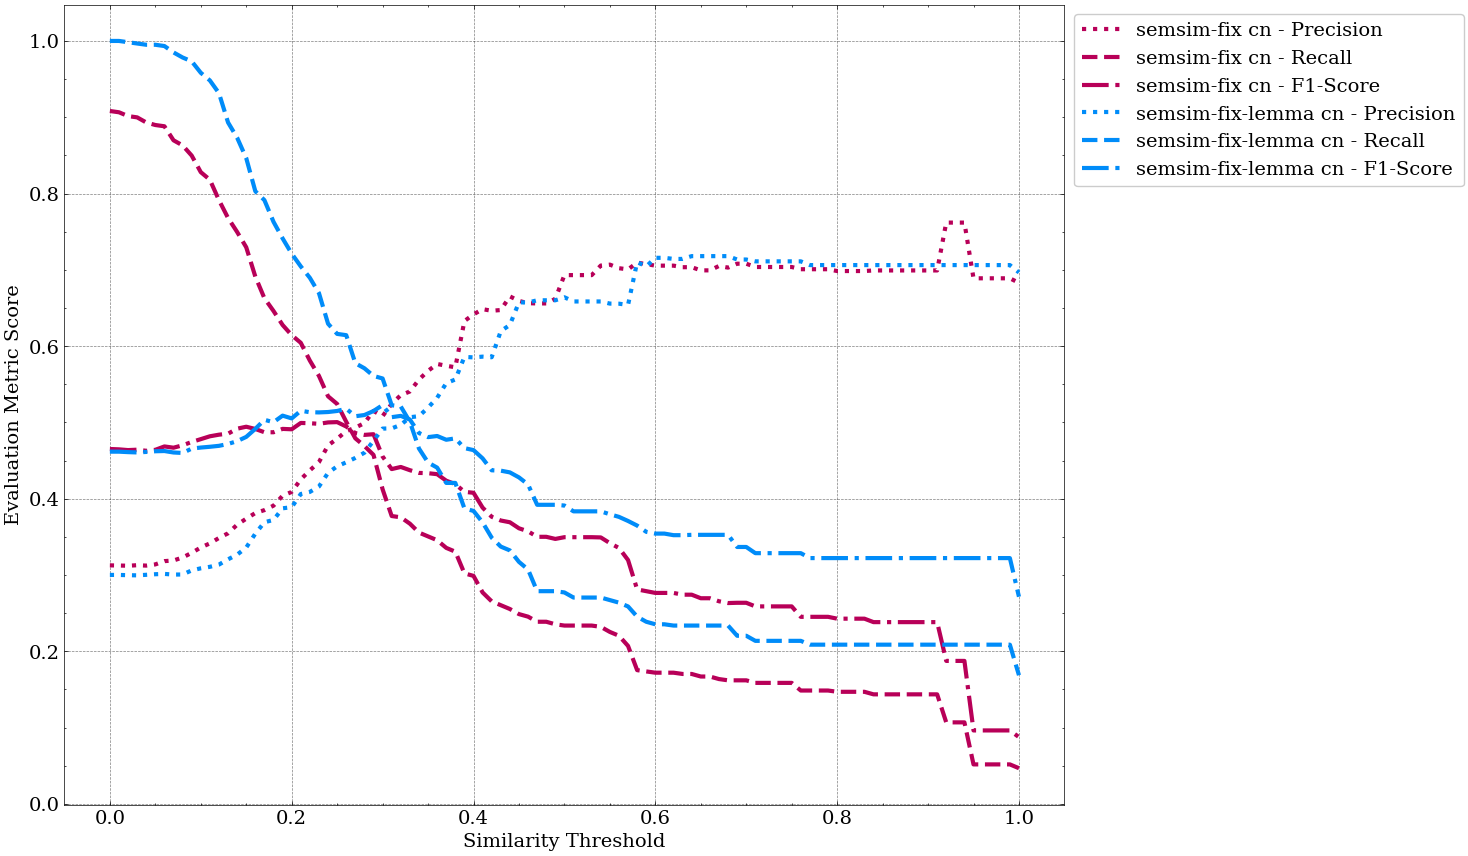
\includegraphics[width=\textwidth]{dataset_conflicts_1-2_pred_wildcard_subsample-2000_evaluation_semsim-fix_cn_vs_semsim-fix-lemma_cn_precision-recall-f1}
\caption{Precision, recall and F1-score vs. ST for the evaluation runs \texttt{semsim-fix cn} and \texttt{semsim-fix-lemma cn}}
\label{fig:prec-rec-f1-semsim-fix-lemma}
\end{figure}

\begin{figure}[H]
\centering
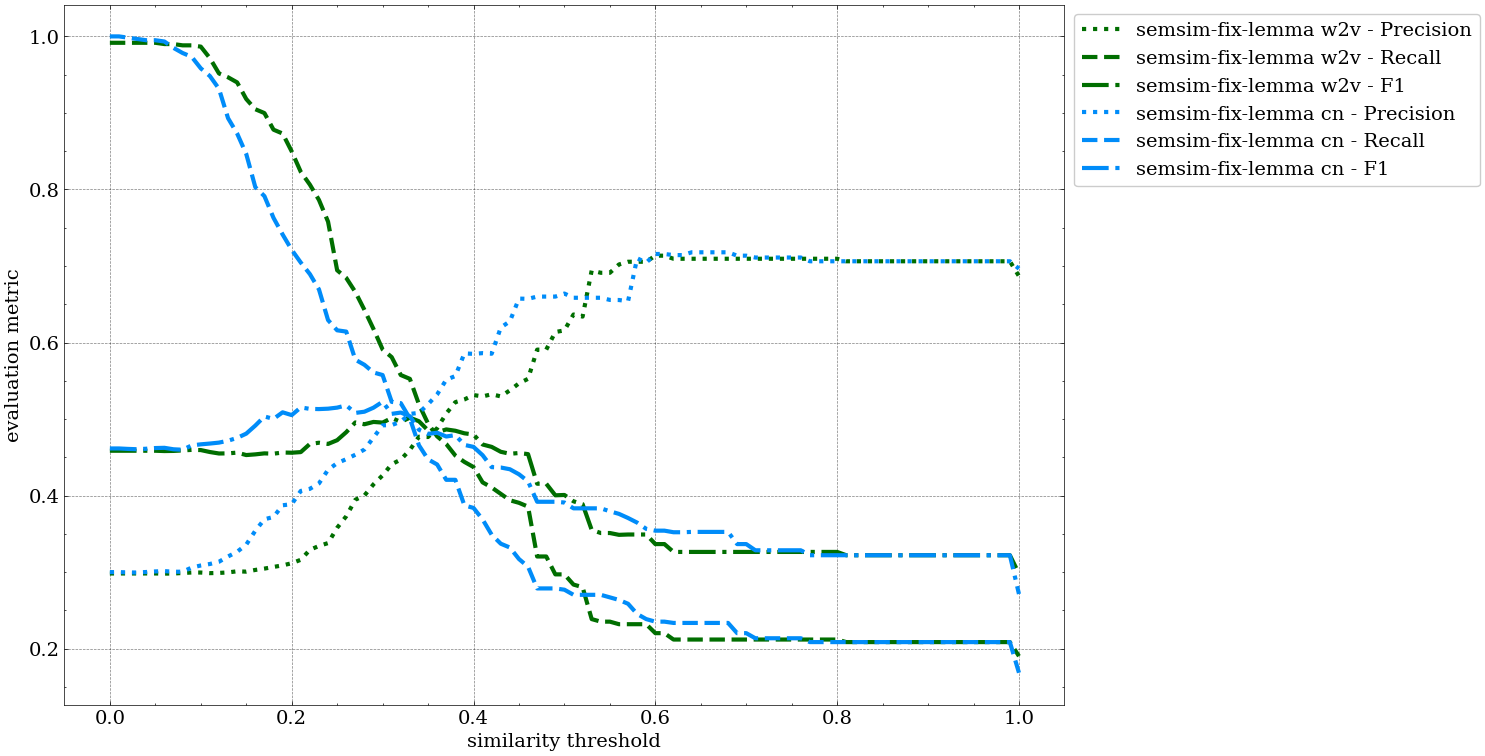
\includegraphics[width=\textwidth]{dataset_conflicts_1-2_pred_wildcard_subsample-2000_evaluation_semsim-fix-lemma_w2v_cn_precision-recall-f1}
\caption{Precision, recall and F1-score vs. ST for the evaluation runs \texttt{semsim-fix-lemma w2v} and \texttt{semsim-fix-lemma cn}}
\label{fig:prec-rec-f1-semxim-fix-lemma-model}
\end{figure}

\begin{figure}[H]
\centering
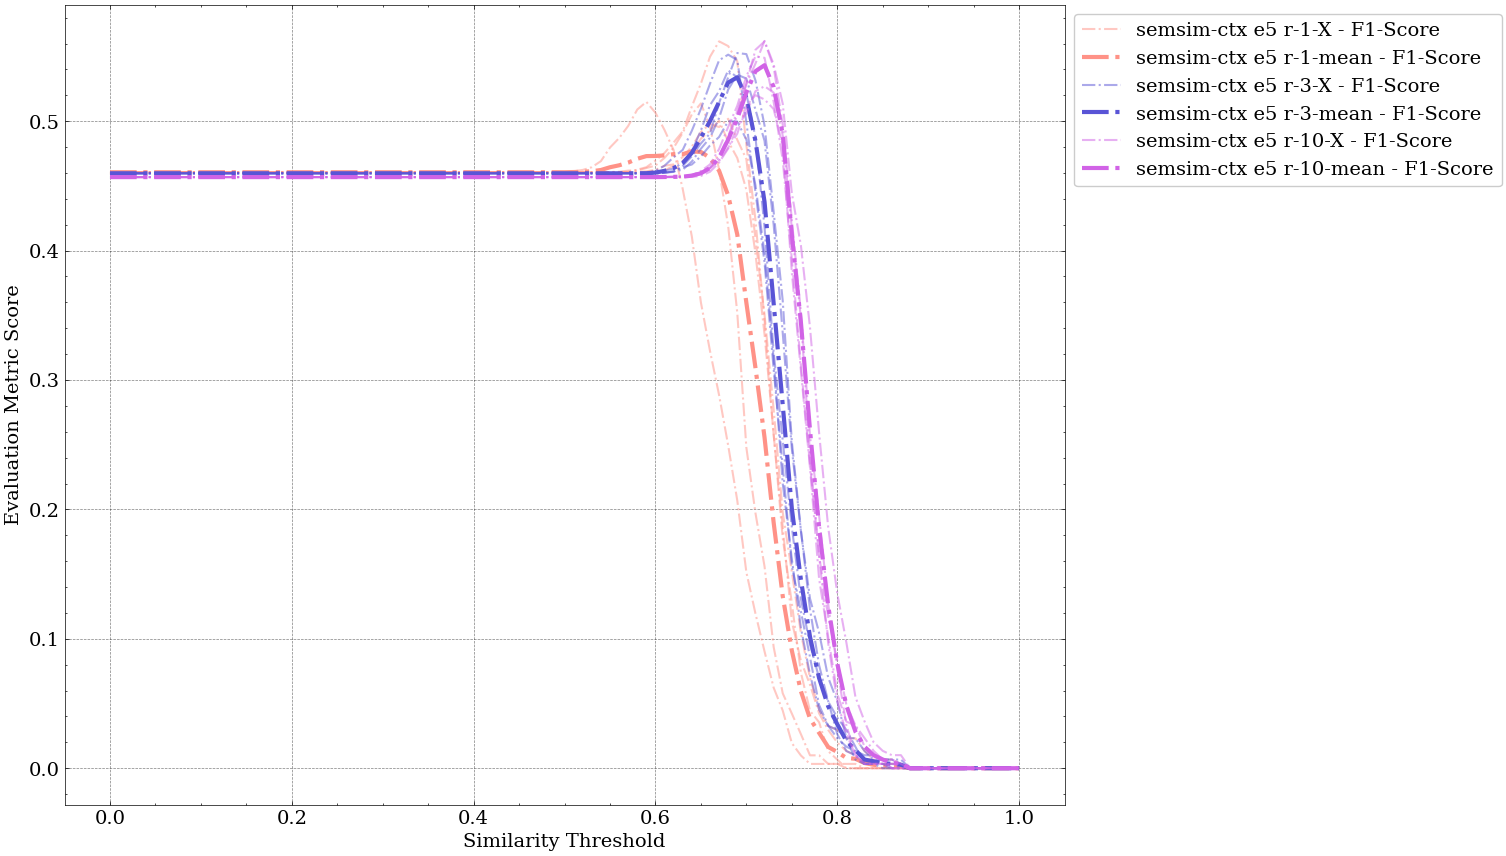
\includegraphics[width=\textwidth]{dataset_conflicts_1-2_pred_wildcard_subsample-2000_evaluation_semsim-ctx_e5_nref-1_vs_nref-3_vs_nref-10_f1}
\caption{F1-score vs. ST for the evaluation runs \texttt{semsim-ctx e5 r-1-X}, \texttt{semsim-ctx e5 r-3-X} and \texttt{semsim-ctx e5 r-10-X}}
\label{fig:f1-semsim-ctx-nref}
\end{figure}

\begin{figure}[H]
\centering
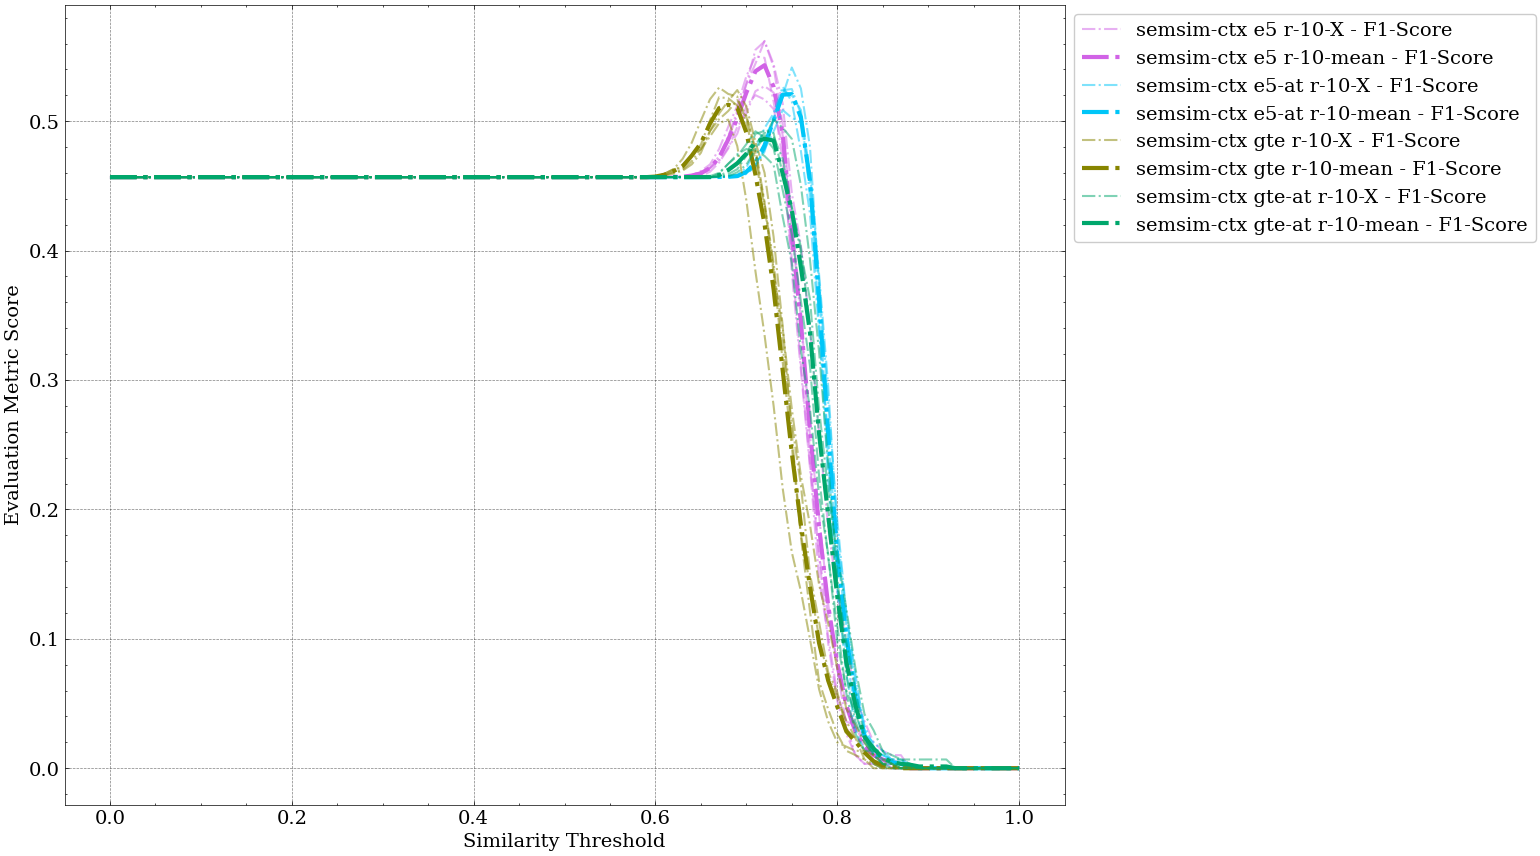
\includegraphics[width=\textwidth]{dataset_conflicts_1-2_pred_wildcard_subsample-2000_evaluation_semsim-ctx_nref-10_e5_e5-at_gte_gte-at_f1}
\caption{F1-score vs. ST for the evaluation runs \texttt{semsim-ctx e5 r-10-X}, \texttt{semsim-ctx e5-at r-10-X}, \texttt{semsim-ctx gte r-10-X} and \texttt{semsim-ctx gte-at r-10-X}}
\label{fig:f1-semsim-ctx-model-at}
\end{figure}

\begin{figure}[H]
\centering
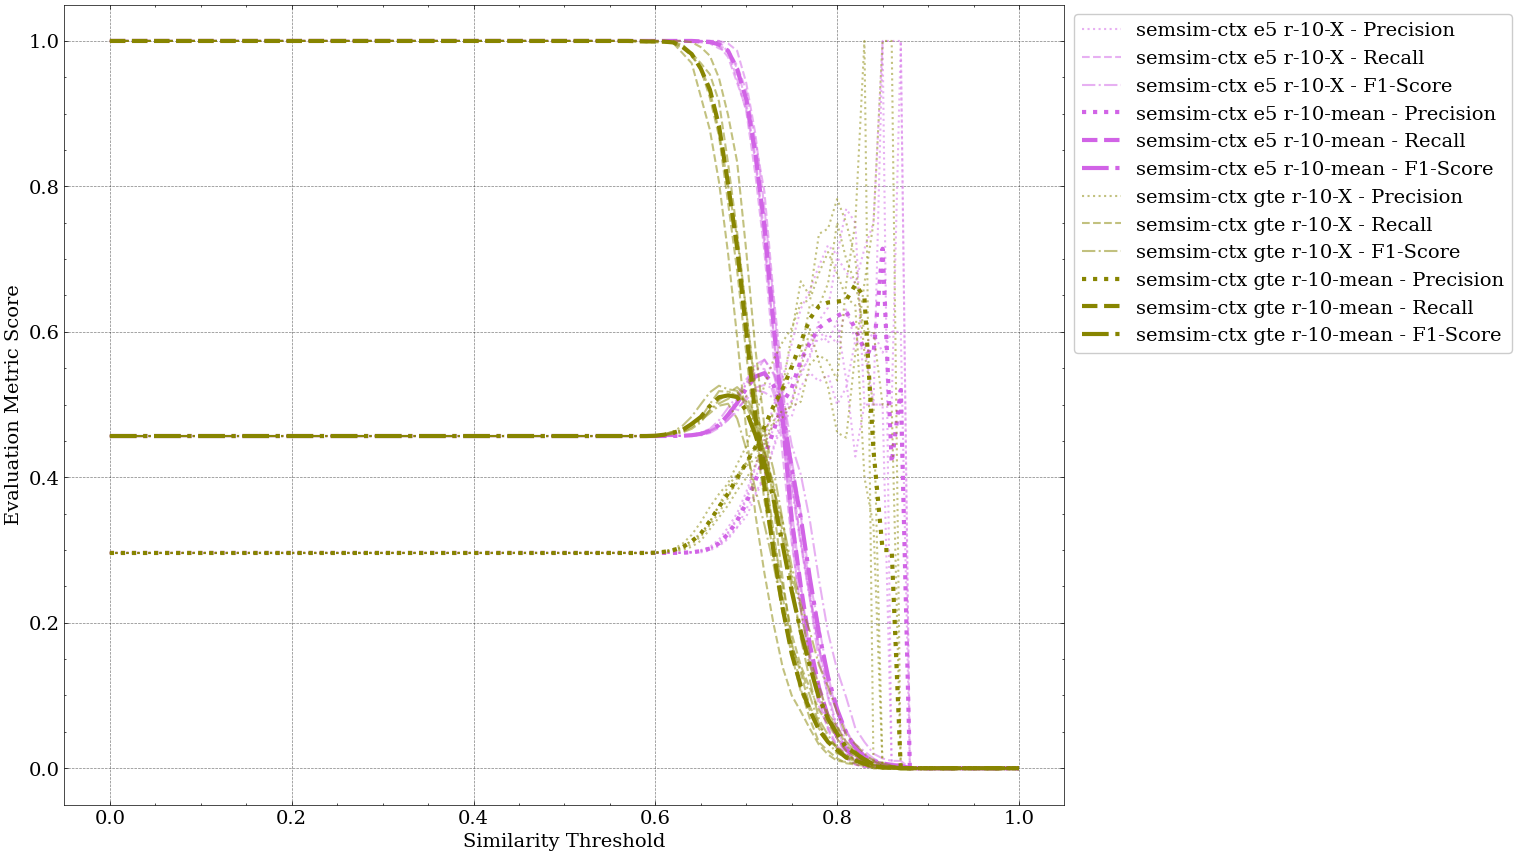
\includegraphics[width=\textwidth]{dataset_conflicts_1-2_pred_wildcard_subsample-2000_evaluation_semsim-ctx_nref-10_e5_vs_gte_precision-recall-f1}
\caption{Precision, recall and F1-score vs. ST for the evaluation runs \texttt{semsim-ctx e5 r-10-X} and \texttt{semsim-ctx gte r-10-X}}
\label{fig:prec-rec-f1-semsim-ctx-model}
\end{figure}

\begin{figure}[H]
\centering
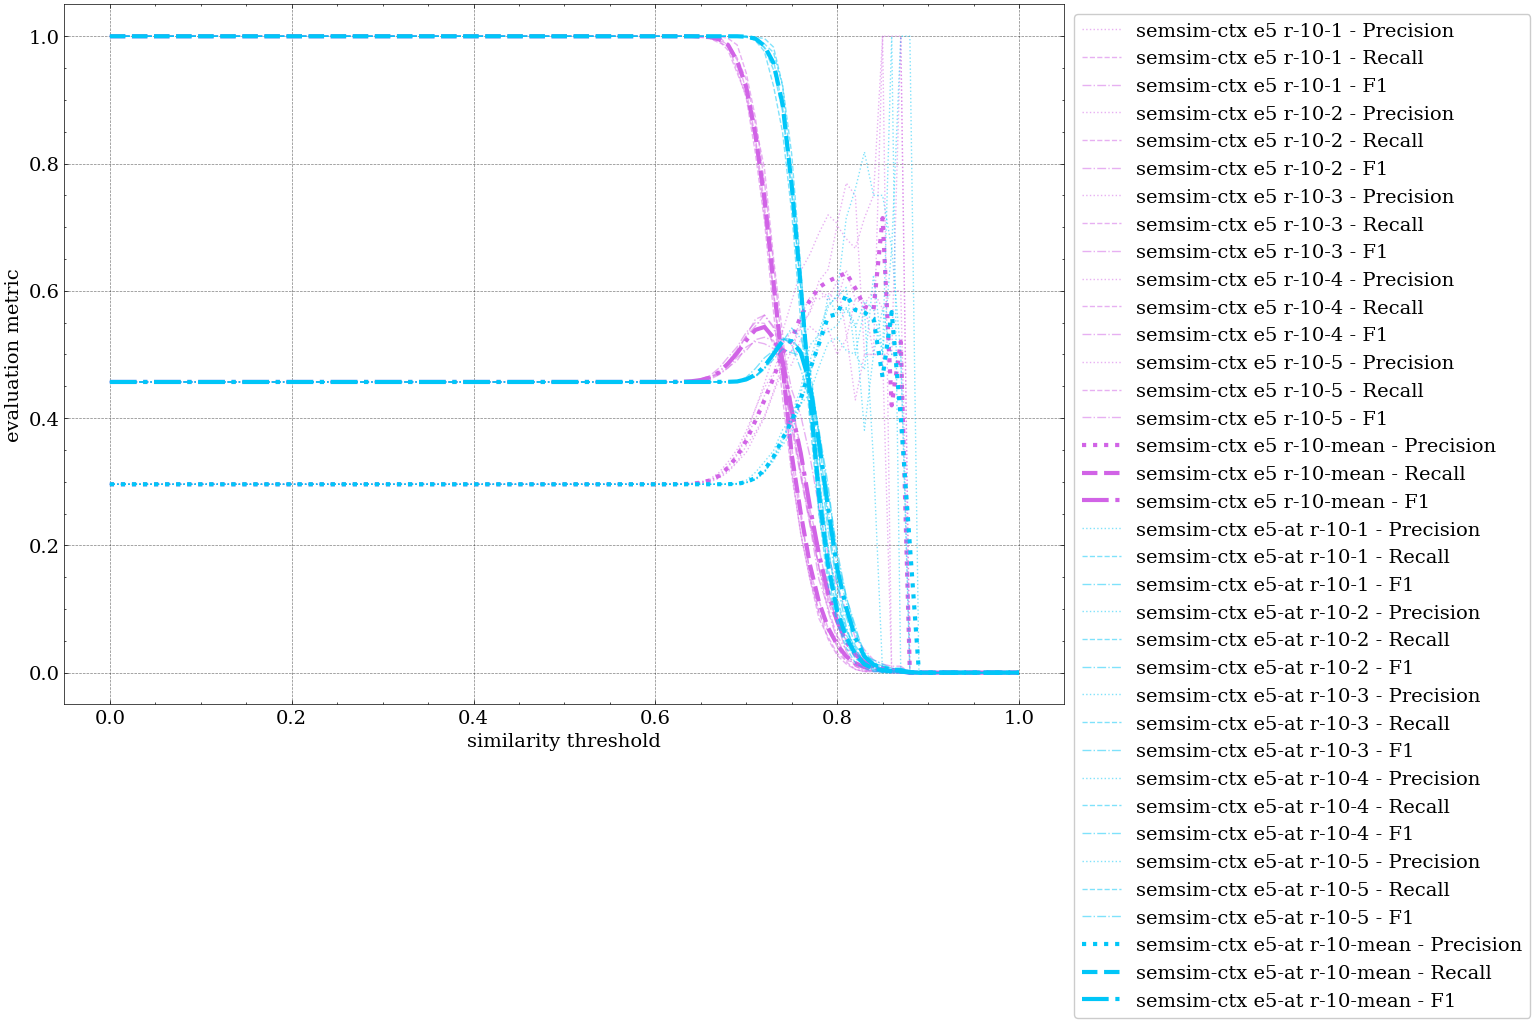
\includegraphics[width=\textwidth]{dataset_conflicts_1-2_pred_wildcard_subsample-2000_evaluation_semsim-ctx_nref-10_e5-vs_e5-at_precision-recall-f1}
\caption{Precision, recall and F1-score vs. ST for the evaluation runs \texttt{semsim-ctx e5 r-10-X} and \texttt{semsim-ctx e5-at r-10-X}}
\label{fig:prec-rec-f1-semsim-ctx-at}
\end{figure}



%\newpage
%\section{PLES Evaluation Label Comparison Tables}
%\label{app-sec:ples-eval-labels}
%
%\begin{sidewaystable}[htp]
%\centering
%\begin{tabular}{l p{13cm} ccc}
%\toprule
%Lemma (\(n\_s\)) & Edge Content & Label Dataset & Label Eval. A & Label Eval. B \\
%\midrule
%capture (7) & Video captures horror of Istanbul airport attack & no conflict & conflict & no conflict) \\
%& Syrian Troops Capture Village Near Northern City of Aleppo & no conflict & conflict & no conflict \\
%& Iraqi forces capture key parts of Mosul neighborhood & no conflict & conflict & no conflict \\
%& Iraqi forces capture west Mosul's main buildings in pre-dawn raid & no conflict & conflict & no conflict \\
%& The videos capture 10 seconds of movement, just enough to catch trucks’ license plates—the operation’s main objective & no conflict & conflict & no conflict \\
%& Security Service of Ukraine Captured Russian Spy & conflict & conflict & conflict \\
%& Syrian Army strikes back in Deir Ezzor: Tal Barouk captured (Report + Video & conflict & conflict & no conflict \\
%\hline
%accept (7)
%& Saudi blogger Badawi's wife accepts Sakharov Prize & no conflict & conflict & no conflict \\
%& UK accepts 1,500 asylum seekers from Syria & no conflict & conflict & no conflict \\
%& Syria rebel chief rejects US-Russia chemical arms deal — “We cannot accept any part of this initiative & conflict & conflict & conflict \\
%& Catholic hospitals accept birth control compromise & no conflict & conflict & conflict \\
%& Japan accepts less than 1\% of asylum applications & no conflict & conflict & no conflict \\
%& Nato accepts Afghan leader Karzai's air strikes decree & no conflict & conflict & no conflict \\
%& S. Korea accepts North's Sunday talks proposal, calls for Panmunjom meeting & no conflict & conflict & no conflict \\
%\hline
%detain (5)
%& Syrian rebels detain U.N. peacekeepers & conflict & conflict & no conflict \\
%& Russian police detain several gay activists & conflict & conflict & conflict \\
%& Mexico detains growing number of undocumented Cubans & conflict & conflict & conflict \\
%& India releases detained Iranian ship & no conflict & conflict & no conflict \\
%& Police in China have detained six executives of a meat supply company that supplied long-expired meat to foreign fast food chains McDonald’s and KFC-parent Yum Brands Inc, among many others & conflict & conflict & conflict \\
%\bottomrule
%\end{tabular}
%\caption{Dataset labels and evaluation labels for edges corresponding to predicate lemmas with the highest abs. diff. in precision between the evaluation runs with recall \(> 0\) and number of samples per lemma \(n_s >= 5\) for the evaluation runs \texttt{semsim-fix-lemma cn t-0.30} (A) and \texttt{semsim-ctx e5 r-10-2 t-0.72} (B)  (Num. one to five of top ten lemmas)}
%\label{tab:ples-labels-1}
%\end{sidewaystable}
%
%
%\begin{sidewaystable}[ht]
%\centering
%\begin{tabular}{l p{13cm} ccc}
%\toprule
%Lemma (\(n\_s\)) & Edge Content & Label Dataset & Label Eval. A & Label Eval. B \\
%\midrule
%deny (20)
%& Syrian officials deny chemical weapon use & no conflict & conflict & conflict \\
%& Germany, EU deny report on European solidarity tax & no conflict & conflict & conflict \\
%& Tebus deny rumours about handing over the last base & no conflict & conflict & no conflict \\
%& Toronto mayor Rob Ford reportedly denied entry to US & conflict & conflict & conflict \\
%& Kenya to deny entry to Ebola states & conflict & conflict & conflict \\
%& The Vatican has categorically denied a report in an Italian newspaper that Pope Francis might have a small, yet curable brain tumor & no conflict & conflict & no conflict \\
%& Indian government denies renewal of passport opposition lawyer over minor traffic rule violation & conflict & conflict & no conflict \\
%& Mexican judge denies El Chapo's appeals against extradition & conflict & conflict & conflict \\
%& Syria denies use of any chemical weapons & no conflict & conflict & conflict \\
%& Toronto mayor denies existence of crack smoking video & no conflict & conflict & no conflict \\
%& North Korea denies responsibility for Sony cyberattack & conflict & conflict & conflict \\
%& Russia denies ground troop in Syria & no conflict & conflict & conflict \\
%& New Pro-Kremlin Crimean Prime Minister Aksyonov denies allegations of criminal past & no conflict & conflict & no conflict \\
%& Free Syrian Army denies responsibility & no conflict & conflict & conflict \\
%& UK defense minister denies report of divisions in PM May's team & no conflict & conflict & no conflict \\
%& Iran denies allegations of organizing spy cell in Nigeria & no conflict & conflict & no conflict \\
%& Russia denies knowledge of arrest ISIS leader Baghdadi & no conflict & conflict & conflict \\
%& Turkish FM denies investigation claims on German firms & no conflict & conflict & no conflict \\
%& Russia Denies Any Role in Deadly Convoy Attack Syria & no conflict & conflict & conflict \\
%& China denies Hong Kong visit request by U.S. carrier group: Pentagon & conflict & conflict & conflict \\
%\bottomrule
%\end{tabular}
%\caption{Dataset labels and evaluation labels for edges corresponding to predicate lemmas with the highest abs. diff. in precision between the evaluation runs with recall \(> 0\) and number of samples per lemma \(n_s >= 5\) for the evaluation runs \texttt{semsim-fix-lemma cn t-0.30} (A) and \texttt{semsim-ctx e5 r-10-2 t-0.72} (B)  (Num. four of top ten lemmas)}
%\label{tab:ples-labels-2}
%\end{sidewaystable}
%
%
%\begin{sidewaystable}[ht]
%\centering
%\begin{tabular}{l p{13cm} ccc}
%\toprule
%Lemma (\(n\_s\)) & Edge Content & Label Dataset & Label Eval. A & Label Eval. B \\
%\midrule
%\hline
%attack (12)
%& Pussy Riot members attack bandmates for appearing at Amnesty concert & conflict & conflict & conflict \\
%& Israelis Attack Palestinian Farmers near Hebron & conflict & conflict & conflict \\
%& Yemeni forces attack sixth Saudi warship & conflict & conflict & conflict \\
%& Passengers attack Edinburgh taxi driver & conflict & conflict & conflict \\
%& Angry Palestinians Attack Hamas Official Over Gaza Destruction & conflict & conflict & conflict \\
%& Israeli Air Force attacks Assad army targets & conflict & conflict & conflict \\
%& They Beat Me’: Univision Reporter Attacked Outside Venezuelan Supreme Court & no conflict & conflict & no conflict \\
%& Locals attack police to foil casino raid & conflict & conflict & conflict \\
%& Afghans attack Indian consulate & conflict & conflict & conflict \\
%& Suspected PKK supporters attack Turkish building in Germany & conflict & conflict & conflict \\
%& Paris attacks a reaction to US actions in Syria, Iraq: Indian Minister & no conflict & conflict & no conflict \\
%& Muslim mob attacks Mosque in Pakistan & conflict & conflict & conflict \\
%\hline
%strike (9)
%& Ex-Muslim poet strikes fear in PC Denmark & conflict & conflict & no conflict \\
%& Double hotel bombing strikes Iraqi capital & no conflict & conflict & conflict \\
%& Magnitude 6.9 quake strikes Sichuan region of China & no conflict & conflict & conflict \\
%& Syrian Israel strikes Syrian targets & conflict & conflict & conflict \\
%& Israeli warplanes strike Syrian weapons facility & conflict & conflict & conflict \\
%& U.S. planes strike militants near Iraq's Amreli, airdrop aid & conflict & conflict & no conflict \\
%& Fake threats strike fear for Sochi Olympic Security & no conflict & conflict & conflict \\
%& UK strikes first ISIS targets & conflict & conflict & no conflict \\
%& Iraqi Army strikes 3 Islamic State strongholds & conflict & conflict & conflict \\
%\hline
%suggest (5)
%& Turkish state news agency suggests link between Boko Haram and Western interests in Nigerian oil & no conflict & conflict & conflict \\
%& New study suggests more and longer atmospheric stagnation events due to global warming & no conflict & conflict & no conflict \\
%& A prominent Iranian official recently suggested a new drug policy for the country that includes taking steps toward the legalization of cannabis and opium & no conflict & conflict & no conflict \\
%& U.N. aid chief suggests more intervention in humanitarian emergencies & no conflict & conflict & conflict \\
%& North Korea's behavior suggests a possible EMP strike against the U.S. & conflict & conflict & conflict \\
%\bottomrule
%\end{tabular}
%\caption{Dataset labels and evaluation labels for edges corresponding to predicate lemmas with the highest abs. diff. in precision between the evaluation runs with recall \(> 0\) and number of samples per lemma \(n_s >= 5\) for the evaluation runs \texttt{semsim-fix-lemma cn t-0.30} (A) and \texttt{semsim-ctx e5 r-10-2 t-0.72} (B)  (Num. five to seven of top ten lemmastop ten lemmas)}
%\label{tab:ples-labels-3}
%\end{sidewaystable}
%
%
%\begin{sidewaystable}[ht]
%\centering
%\begin{tabular}{l p{13cm} ccc}
%\toprule
%Lemma (\(n\_s\)) & Edge Content & Label Dataset & Label Eval. A & Label Eval. B \\
%\midrule
%claim (22)
%& Chevron claims new proof of fraud in Ecuador pollution ruling & no conflict & conflict & no conflict \\
%& Iran claims new generation of 15-times-faster centrifuges & no conflict & conflict & no conflict \\
%& A prolonged drought in Brazil has already claimed about half of Jose Francisco Pereira’s coffee crop & no conflict & conflict & no conflict \\
%& ISIS backers claim responsibility for Paris-style terror attack in Jakarta & no conflict & conflict & conflict \\
%& Salafist group claims responsibility for bombing French center in Gaza & no conflict & conflict & conflict \\
%& Rockets fired on southern Israel from Sinai, ISIS claims responsibility & conflict & conflict & conflict \\
%& ISIS claim responsibility for Paris terror attacks in online statement & no conflict & conflict & conflict \\
%& Isis claims responsibility for Paris shooting attack that left one police officer dead & no conflict & conflict & conflict \\
%& Convicted Israeli trainer of Colombia paramilitaries claims CIA ties & no conflict & conflict & no conflict \\
%& Pakistan Taliban faction claims park attack on Lahore Christians & conflict & conflict & conflict \\
%& Burundi Rebels Claim Rwanda Military Training & no conflict & conflict & conflict \\
%& Isis claims responsibility for killing of Hindu priest in Bangladesh & conflict & conflict & conflict \\
%& PKK-linked TAK claims responsibility for Ankara attack & no conflict & conflict & conflict \\
%& Ansar Bayt al-Maqdis claims responsibility for opening fire on Israeli soldiers near Egyptian border & conflict & conflict & conflict \\
%& Sectarian war an aim of Gulf states, Israel and Turkey, claims Hezbollah & conflict & conflict & conflict \\
%& Iran Sunni group Jaish al-Adl claims border attack & no conflict & conflict & conflict \\
%& ISIS Claims Responsibility In Turkish Nightclub Attack; U.S. Man Among The Wounded & conflict & conflict & conflict \\
%& Bangkok police claim reward in Erawan Shrine bomber hunt & no conflict & conflict & no conflict \\
%& Taliban claim Kabul attack & no conflict & conflict & conflict \\
%& Denmark claims north pole & no conflict & conflict & no conflict \\
%& WikiLeaks' Julian Assange Claims Vindication in UN Ruling & no conflict & conflict & conflict \\
%& ISIS claims responsibility for Eilat rockets & no conflict & conflict & conflict \\
%\bottomrule
%\end{tabular}
%\caption{Dataset labels and evaluation labels for edges corresponding to predicate lemmas with the highest abs. diff. in precision between the evaluation runs with recall \(> 0\) and number of samples per lemma \(n_s >= 5\) for the evaluation runs \texttt{semsim-fix-lemma cn t-0.30} (A) and \texttt{semsim-ctx e5 r-10-2 t-0.72} (B)  (Num. eight of top ten lemma)}
%\label{tab:ples-labels-4}
%\end{sidewaystable}
%
%
%\begin{sidewaystable}[ht]
%\centering
%\begin{tabular}{l p{13cm} ccc}
%\toprule
%Lemma (\(n\_s\)) & Edge Content & Label Dataset & Label Eval. A & Label Eval. B \\
%\midrule
%threaten (20)
%& North Korea Threatens To "Invade USA," Use Weapons "Unknown To The World & conflict & conflict & conflict \\
%& FATCA threatens Russia’s financial system – official & conflict & conflict & conflict \\
%& Wartime economic crisis threatens education of millions Yemeni children & no conflict & conflict & no conflict \\
%& Syria opposition threatens withdrawal from Geneva talks & no conflict & conflict & conflict \\
%& Al-Qaeda affiliates are threatening West Africa’s most peaceful cities & conflict & conflict & conflict \\
%& Video threatens Sochi Winter Olympics & no conflict & conflict & conflict \\
%& Ukraine crisis threatens Transnistria & no conflict & conflict & conflict \\
%& Giant comets may threaten Earth & no conflict & conflict & no conflict \\
%& Protests in Turkey Threaten Erdogans Political Future & conflict & conflict & conflict \\
%& Brazil Rejects Israel's Ambassador; Israel Threatens Relations Downgrade : NPR \& conflict & conflict & conflict \\
%& North Korea Threatens 'Merciless' Strike Against US-South Korea Drill & conflict & conflict & conflict \\
%& Kim Dotcom case threatens New Zealand Government & no conflict & conflict & conflict \\
%& Proposed German legislation threatens broad internet censorship & no conflict & conflict & conflict \\
%& Abe government threatens NHKs credibility & no conflict & conflict & conflict \\
%& British ISIS fighter 'Al-Britani' threatens executions in Trafalgar Square & no conflict & conflict & conflict \\
%& How one racy condom ad may threaten gains female sex education in Pakistan & no conflict & conflict & no conflict \\
%& Police Use of Drones May Threaten Human Rights: UN Expert \& no conflict & conflict & conflict \\
%& North Korea threatens pre-emptive nuke strike against U.S. \& S. Korea & conflict & conflict & conflict \\
%& Asylum seekers threaten hunger strike & no conflict & conflict & conflict \\
%& Withdrawal of foreign troops from Afghanistan threatens rollback of women's gains & no conflict & conflict & no conflict \\
%\bottomrule
%\end{tabular}
%\caption{Dataset labels and evaluation labels for edges corresponding to predicate lemmas with the highest abs. diff. in precision between the evaluation runs with recall \(> 0\) and number of samples per lemma \(n_s >= 5\) for the evaluation runs \texttt{semsim-fix-lemma cn t-0.30} (A) and \texttt{semsim-ctx e5 r-10-2 t-0.72} (B)  (Num. nine of top ten lemma)}
%\label{tab:ples-labels-5}
%\end{sidewaystable}
%
%
%\begin{sidewaystable}[ht]
%\centering
%\begin{tabular}{l p{13cm} ccc}
%\toprule
%Lemma (\(n\_s\)) & Edge Content & Label Dataset & Label Eval. A & Label Eval. B \\
%\midrule
%say (16 of 31)
%& Iran says no snap inspections of nuclear sites & no conflict & conflict & no conflict \\
%& Child abuse image investigation leads to 660 arrests: UK National Crime Agency said the 660 arrested included doctors, teachers, scout leaders, care workers and former police officers & no conflict & conflict & no conflict \\
%& Former Cuba Leader Fidel Castro Says 'Israel and US Fathered Isis & no conflict & conflict & conflict \\
%& Malaysian court to Christians: You can't say 'Allah & conflict & conflict & conflict \\
%& U.S. State Dept. says "confident" Russian gov & no conflict & conflict & conflict \\
%& State Border Service says Russian troops still near Ukraine's border & no conflict & conflict & no conflict \\
%& France military says Mali town Konna 'not recaptured' from Islamists denying an earlier claim by the Malian army & conflict & conflict & no conflict \\
%& Thai PM says occupation of state buildings threat to stability & no conflict & conflict & conflict \\
%& Australia says Chinese spy ship near war games & no conflict & conflict & no conflict \\
%& Denmark Says Microsoft Owes  £660 Million in Tax & conflict & conflict & no conflict \\
%& Japan Says Armed Chinese Ship Infiltrates Its Territorial Waters & conflict & conflict & conflict \\
%& EU report says LGBT face discrimination & no conflict & conflict & conflict \\
%& Group says boycott Qatar Airways, cites poor rights record & conflict & conflict & conflict \\
%& WHO incapable of reacting to crises such as Ebola, says report & no conflict & conflict & no conflict \\
%& Migrant ship off Greece says armed people on board & no conflict & conflict & conflict \\
%& Turkey says attacks on Aleppo a crime against humanity & no conflict & conflict & conflict \\
%\bottomrule
%\end{tabular}
%\caption{Dataset labels and evaluation labels for edges corresponding to predicate lemmas with the highest abs. diff. in precision between the evaluation runs with recall \(> 0\) and number of samples per lemma \(n_s >= 5\) for the evaluation runs \texttt{semsim-fix-lemma cn t-0.30} (A) and \texttt{semsim-ctx e5 r-10-2 t-0.72} (B)  (Num. ten of top ten lemma)}
%\label{tab:ples-labels-6}
%\end{sidewaystable}
%
%
%\begin{sidewaystable}[ht]
%\centering
%\begin{tabular}{l p{13cm} ccc}
%\toprule
%Lemma (\(n\_s\)) & Edge Content & Label Dataset & Label Eval. A & Label Eval. B \\
%\midrule
%say (15 of 31)
%& Mystery man in Bangkok bomb probe 'never said a word & no conflict & conflict & no conflict \\
%& I Recant Says Author of Infamous Seventies Newsweek Global Cooling Article & no conflict & conflict & no conflict \\
%& Sister says don't make missing Flight 370 pilot the fall guy & no conflict & conflict & no conflict \\
%& VW works council says talks over strategy pact broken off without results & no conflict & conflict & no conflict \\
%& Head of Russia's Rosneft says U.S., not OPEC, Rules Oil Markets & no conflict & conflict & no conflict \\
%& Indian textbook says "Japan Nuked US & no conflict & conflict & no conflict \\
%& North Korea says US sanctions on leader "a declaration of war & conflict & conflict & conflict \\
%& President of Gambia says homosexuality one of three greatest threats to humanity & conflict & conflict & conflict \\
%& China Says Its Working with Latin America for a New World Order & no conflict & conflict & conflict \\
%& Myanmar Parliament Chairman Says Nominees for Country's Next President, 2 Vice Presidents Will Be Revealed March 17 & no conflict & conflict & no conflict \\
%& G7 says no sanctions on Russia over Syria & no conflict & conflict & conflict \\
%& South Korea's Lotte Duty Free says China cyber attacks crashed website & conflict & conflict & no conflict \\
%& Kuwait says stateless to be offered Comoros citizenship & no conflict & conflict & conflict \\
%& Syria Says Israel Attacked Military Airport & conflict & conflict & conflict \\
%& Bainimarama says NZ easing of sanctions 'insincere & no conflict & conflict & conflict \\
%\bottomrule
%\end{tabular}
%\caption{Dataset labels and evaluation labels for edges corresponding to predicate lemmas with the highest abs. diff. in precision between the evaluation runs with recall \(> 0\) and number of samples per lemma \(n_s >= 5\) for the evaluation runs \texttt{semsim-fix-lemma cn t-0.30} (A) and \texttt{semsim-ctx e5 r-10-2 t-0.72} (B)  (Num. ten of top ten lemma)}
%\label{tab:ples-labels-7}
%\end{sidewaystable}




\end{document}
 